% !TEX encoding = UTF-8 Unicode
% !TEX TS-program = pdflatex

% toptesti document class
\documentclass[%
    a4paper, % not needed, by default it is a4paper, or also b5paper can be used
    corpo=10pt, % dimension of basic font
    % oneside is generally the way to go
    oneside, % two side optimizes for two-face printing, having chapters open on the right (aka odd numbers), if you don't want blank pages put oneside here
    stile=standard,
    %evenboxes, % not needed, to put supervisors and candidate at the same level
    tipotesi=magistrale,
    numerazioneromana, % roman numbering for appendixes and preambles, up to Table of Contents
    openright, % to force opening on the right for double-sided printing
    cucitura=7mm, % for printing, 7mm should be enough
    %dvipsnames, % for compatibility with xcolor, it does not work
]{toptesi}

%%%%%%%%%%%%%%%%%%%%%%%%%%%%%%%%%%%%%%%%%%%%%%%%%%%%
\usepackage[english]{babel}
\usepackage[utf8]{inputenc}
\usepackage[T1]{fontenc}
\usepackage{lmodern}

\usepackage{hyperref} % must be loaded before glossaries-extra

% bibliography
\usepackage[hyperref=true,backref=true,backend=biber,maxbibnames=9,maxcitenames=2,style=numeric,citestyle=numeric,sorting=none]{biblatex} % hyperref uses links, backref goes back to citations, uses biber as backend, with 9 names at most in bibliography and 2 in citations, citing using numbers, and sorting in citation order
% sorting can be also ydnt for year descending, name, title or ynt for ascending year

\usepackage{adjustbox} % to resize boxes by keeping the same aspect ratio
\usepackage{algorithm} % algorithm environment
\usepackage{algpseudocode} % improved pseudo-code
\usepackage{amsfonts}               %  AMS mathematical fonts
\usepackage{amsmath}
\usepackage{amssymb}                %  AMS mathematical symbols
\usepackage{bm}                     %  black/bold mathematical symbols
\usepackage{booktabs}               %  better tables
\usepackage[labelfont=bf]{caption} % font=footnotesize % to have reduced caption font size
\usepackage{csquotes}
\usepackage{enumitem} %left align the bulleted points
\usepackage{geometry}
%\usepackage{glossaries} % to use acronyms and glossary, it has also glossaries-extra as extension, but commands are different
\usepackage[%
    toc, % puts the link in the ToC
    %record, % to use bib2gls
    abbreviations, % to load abbreviations / acronyms
    nonumberlist, % to avoid printing the numbers of the references in the acronyms page
]{glossaries-extra}
\usepackage{graphicx}               %  post-script images
%\usepackage{iwona} % extra fonts, substitute standard ones
\usepackage{listings} % to insert formatted code
\usepackage{lipsum} % for lorem ipsum text, not needed in the real work
\usepackage{makecell} % to change dimensions of cells, for math cases
\usepackage{mathtools} % for additional commands
\usepackage{mfirstuc} % to have capitalization capabilities
\usepackage[final]{microtype}      % microtypography, final lets latex use it also in bibliography
\usepackage{multirow} % to allow for cells covering more than 1 row in tables
\usepackage{nicefrac}       % compact symbols for 1/2, etc.
%\usepackage[lofdepth,lotdepth]{subfig}
\usepackage{ragged2e} % for justifying text
\usepackage{siunitx} % support for SI units of measurement and number typesetting
\usepackage{subfig}
\usepackage{svg} % for svg support, works only if inkscape is installed, default for Overleaf v2
%\usepackage{subfigure}              %  subfigure compatibility, can be removed if subfig
\usepackage{tabularx} % equal-width columns in tables
\usepackage{textcomp} % extra fonts and symbols
\usepackage{url}            % simple URL typesetting
\usepackage{verbatim} % for extended verbatim support
\usepackage{xcolor} % to define colors and use standard CSS names add dvipsnames as option, but it clashes with xcolor loaded in toptesi, pay attention that if it goes in conflict with tikz/beamer, simply use \documentclass[usenames,dvipsnames]{beamer}, along with other custom options when defining the document class


% configuration for glossaries
% convert and load converted glossaries in .tex ,format from .bib
\setabbreviationstyle{long-short-desc} % style before loading resources
% this command sets the style to title for long names of acronyms only in the glossary description, leading to capitalized first-letter for all words
% \glssetcategoryattribute{\glsxtrabbrvtype}{glossname}{capitalisewords} % doesn't work
% resources to load if using a bib file with bib2gls
%\GlsXtrLoadResources[%
% src={glossaries}, % name of the file without extension
% selection=all, % select all the entries
%]
% not needed
%\newglossary*{abbreviation}{Acronyms} % to change the name of this glossary for acronyms

%\renewcommand{\glsclearpage}{\paginavuota} % to allow glossaries to clear pages, done manually is better


% setup for hyperref
\hypersetup{%
    pdfpagemode={UseOutlines},
    bookmarksopen,
    pdfstartview={FitH},
    colorlinks,
    linkcolor={black}, % it is suggested to keep them black, since when printing it it costs per page, and if they have color it's twice the price per page
    citecolor={black},
    urlcolor={black}
  }
%

% setup for svg
\svgsetup{%
    inkscapeformat=pdf, % to force usage of PDF
    inkscapelatex=false, % to disable latex rendering of text, produces errors
}

% setup for siunitx, it does not work in the summary
\sisetup{%
    detect-all, % to use the same font as for writing when using \num
    mode=text, % to allow it to work also in math mode
    group-separator = {,}, % separator for number grouping
    group-minimum-digits = 3, % minimum number of digits a number must have to be grouped in 3-digit groups
}

% listings colours
\definecolor{rulecolor}{rgb}{0,0,0}
\definecolor{commentcolor}{rgb}{0,0.6,0}
\definecolor{linenumbercolor}{rgb}{0.5,0.5,0.5}
\definecolor{keywordcolor}{rgb}{0,0,0.95}
\definecolor{backcolor}{rgb}{1,1,1}%{0.95,0.95,0.92}
\definecolor{stringcolor}{rgb}{0.58,0,0.82}

% setup for lstlisting
\lstset{ %
	backgroundcolor=\color{backcolor},   % choose the background color; you must add \usepackage{color} or \usepackage{xcolor}; should come as last argument
	basicstyle=\footnotesize,        % the size of the fonts that are used for the code
	breakatwhitespace=false,         % sets if automatic breaks should only happen at whitespace
	breaklines=true,                 % sets automatic line breaking
	captionpos=t,                    % sets the caption-position to bottom
	commentstyle=\color{commentcolor},    % comment style
	extendedchars=true,              % lets you use non-ASCII characters; for 8-bits encodings only, does not work with UTF-8
	frame=single,	                   % adds a frame around the code
	keepspaces=true,                 % keeps spaces in text, useful for keeping indentation of code (possibly needs columns=flexible)
	keywordstyle=\color{keywordcolor},       % keyword style
	%language=VHDL,                 % the language of the code
	numbers=left,                    % where to put the line-numbers; possible values are (none, left, right)
	numbersep=5pt,                   % how far the line-numbers are from the code
	numberstyle=\tiny\color{linenumbercolor}, % the style that is used for the line-numbers
	rulecolor=\color{rulecolor},         % if not set, the frame-color may be changed on line-breaks within not-black text (e.g. comments (green here))
	showspaces=false,                % show spaces everywhere adding particular underscores; it overrides 'showstringspaces'
	showstringspaces=false,          % underline spaces within strings only
	showtabs=false,                  % show tabs within strings adding particular underscores
	stepnumber=1,                    % the step between two line-numbers. If it's 1, each line will be numbered
	stringstyle=\color{stringcolor},     % string literal style
	tabsize=4,	                   % sets default tabsize to 2 spaces
	title=\lstname,                   % show the filename of files included with \lstinputlisting; also try caption instead of title
	inputencoding=utf8,
	literate=
	{á}{{\'a}}1 {é}{{\'e}}1 {í}{{\'i}}1 {ó}{{\'o}}1 {ú}{{\'u}}1
	{Á}{{\'A}}1 {É}{{\'E}}1 {Í}{{\'I}}1 {Ó}{{\'O}}1 {Ú}{{\'U}}1
	{à}{{\`a}}1 {è}{{\`e}}1 {ì}{{\`i}}1 {ò}{{\`o}}1 {ù}{{\`u}}1
	{À}{{\`A}}1 {È}{{\'E}}1 {Ì}{{\`I}}1 {Ò}{{\`O}}1 {Ù}{{\`U}}1
	{ä}{{\"a}}1 {ë}{{\"e}}1 {ï}{{\"i}}1 {ö}{{\"o}}1 {ü}{{\"u}}1
	{Ä}{{\"A}}1 {Ë}{{\"E}}1 {Ï}{{\"I}}1 {Ö}{{\"O}}1 {Ü}{{\"U}}1
	{â}{{\^a}}1 {ê}{{\^e}}1 {î}{{\^i}}1 {ô}{{\^o}}1 {û}{{\^u}}1
	{Â}{{\^A}}1 {Ê}{{\^E}}1 {Î}{{\^I}}1 {Ô}{{\^O}}1 {Û}{{\^U}}1
	{œ}{{\oe}}1 {Œ}{{\OE}}1 {æ}{{\ae}}1 {Æ}{{\AE}}1 {ß}{{\ss}}1
	{ű}{{\H{u}}}1 {Ű}{{\H{U}}}1 {ő}{{\H{o}}}1 {Ő}{{\H{O}}}1
	{ç}{{\c c}}1 {Ç}{{\c C}}1 {ø}{{\o}}1 {å}{{\r a}}1 {Å}{{\r A}}1
	{€}{{\euro}}1 {£}{{\pounds}}1 {«}{{\guillemotleft}}1
	{»}{{\guillemotright}}1 {ñ}{{\~n}}1 {Ñ}{{\~N}}1 {¿}{{?`}}1
}


% biblatex setup
% generally 9000 is ok, if higher than 10000 it's bad
% If you want to break on URL numbers
\setcounter{biburlnumpenalty}{9000}
% If you want to break on URL lower case letters
\setcounter{biburllcpenalty}{9000}
% If you want to break on URL UPPER CASE letters
\setcounter{biburlucpenalty}{9000}


\newcommand{\thesisuniversitylogo}{images/logo/polito_logo_2021_blu-2-2} % new PoliTo logo

% how to change Contents to Table of Contents
\addto\captionsenglish{% Replace "english" with the language you use
	\renewcommand{\contentsname}%
	{Table of Contents}%
}

% to change the name of Abbreviations to Acronyms
% not needed if use use entry types and define those
% \renewcommand{\abbreviationsname}{Acronyms}

% to allow line comments in algorithms
\algnewcommand{\LineComment}[1]{\State \(\triangleright\) #1}

% to declare abs and norm
\DeclarePairedDelimiter\abs{\lvert}{\rvert}%
\DeclarePairedDelimiter\norm{\lVert}{\rVert}%

% Swap the definition of \abs* and \norm*, so that \abs
% and \norm resizes the size of the brackets, and the 
% starred version does not.
\makeatletter
\let\oldabs\abs
\def\abs{\@ifstar{\oldabs}{\oldabs*}}
%
\let\oldnorm\norm
\def\norm{\@ifstar{\oldnorm}{\oldnorm*}}
\makeatother


% change this configuration with your info
\newcommand{\thesistitle}{Titolo della tesi}
\newcommand{\thesissubtitle}{Eventuale sottotitolo} % not strictly necessary, leave empty if not needed
\newcommand{\thesiscandidatename}{Name}
\newcommand{\thesiscandidatesurname}{Surname}
\newcommand{\thesissupervisoronename}{Name}
\newcommand{\thesissupervisoronesurname}{Surname}
\newcommand{\thesissupervisortwoname}{Name}
\newcommand{\thesissupervisortwosurname}{Surname}
\newcommand{\thesissupervisorthreename}{Name}
\newcommand{\thesissupervisorthreesurname}{Surname}
\newcommand{\thesisdate}{Mese Anno}
\newcommand{\thesiscourse}{Corso di Laurea}
\newcommand{\academicYear}{A.a. 202x/202x}
\newcommand{\thesisuniversity}{Politecnico di Torino}
\newcommand{\thesiscandidatetext}{Candidati}
\newcommand{\thesissupervisortext}{Relatori}


% fontsize is {size}{spacing}\family
\newcommand {\institutionfont}{\fontsize {20}{30}\scshape}
\newcommand {\divisionfont}{\fontsize {12}{20}\rmfamily}
\newcommand {\pretitlefont}{\fontsize {16}{16}\rmfamily}
\newcommand {\customtitlefont}{\fontsize {24}{28}\scshape}
\newcommand {\customsubtitlefont}{\fontsize {14}{28}\scshape}
% {iwona}{bx}{n}}
\newcommand {\fixednamesfont}{\fontsize {12}{16}\mdseries}
\newcommand {\namesfont}{\fontsize {12}{16}\mdseries}
\newcommand {\footfont}{\fontsize {15}{18}\rmfamily}

\onehalfspacing

\addbibresource{bibliography.bib}

% to load the glossaries, not needed if using bib2gls
% for glossary entry
% @entry{bird,
%     name={bird},
%     description = {feathered animal},
%     see={[see also]{duck,goose}}
% }

% if this bib file does not work, try using \input{file.tex}
% where all the \newabbreviation commands have been inserted
% containing all the definitions

% Gls to capitalize first letter
% GLS for full uppercase
% for abbreviations also
% glsxtrshort for abbreviation
% similar for long, full, and capital configurations, add pl at the end for plurals
% glsentryshort, long, plural (referred to shorts) must be used when in section titles
% glslink to allow the link but use a different text (as for href)


% if you want to use also description for the abbreviations/acronyms, you should use bib2gls and define all the entries in a bib file, which is incompatible with Overleaf
% EXAMPLES
\newacronym{DBMS}{DBMS}{Database Management System}
\makeglossaries

\begin{document}

\overfullrule=0.00001pt % latex shows a black bar for overfulls over this dimension

%\emergencystretch=1em % to allow some stretching in the lines to avoid overfull boxes, also in bibliography, eventually can be used only before bibliography or in the preamble for the whole document, not needed if using biblatex configuration in most cases


%% TOPTESI DEFAULT FRONTPAGE, IGNORED
%\ateneo{\thesisuniversity} % university name
%\logosede[5cm]{\thesisuniversitylogo} % logo, square brackets contain the height

%\titolo{\thesistitle} % title
%\sottotitolo{Metodo dei satelliti medicei} % subtitle

% place/remove a slash \\ to put the name on the following line or after Master Degree Course
%\corsodilaurea{\thesiscourse} % course name


%~251197 % id number is not needed

%\candidato{\thesiscandidatename~\textsc{\thesiscandidatesurname}} % candidate

% using tabular we can have more than 1 supervisor under the same column
%\relatore{\tabular{@{}l}%
%    \xmakefirstuc{\thesissupervisoronetitle}~\thesissupervisoronename~\textsc{\thesissupervisoronesurname}\\[0.4ex]
%    \xmakefirstuc{\thesissupervisortwotitle}~\thesissupervisortwoname~\textsc{\thesissupervisortwosurname}\\[0.4ex]
%    \xmakefirstuc{\thesissupervisorthreetitle}~\thesissupervisorthreename~\textsc{\thesissupervisorthreesurname}
%    \endtabular}
%\terzorelatore{Name}

% in this way we have Academic Year without stile=classica, so without lines
% \sedutadilaurea{\textsc{Academic~Year} 2019-2020}% per la laurea magistrale
% for PoliTo there is only month year
%\sedutadilaurea{\thesisdate}% per la laurea magistrale
% PhD
%\esamedidottorato{Novembre 1610}
%\ciclodidottorato{XV}

% offset for binding, the smaller the better
%\setbindingcorrection{3mm}


%\iflanguage{english}{%
	%\retrofrontespizio{This work is subject to the Creative Commons Licence}

%	\CorsoDiLaureaIn{\thesislevel's Degree Course in\space}

%	\TesiDiLaurea{\thesislevel's Degree Thesis}

%	\InName{in}
%	\CandidateName{\xmakefirstuc{\thesiscandidatetext}}% or Candidates
%	\AdvisorName{\xmakefirstuc{\thesissupervisortext}}% or Supervisor
	%\TutorName{Tutor}
	%\NomeTutoreAziendale{Internship Tutor}

	%\NomePrimoTomo{First volume}
	%\NomeSecondoTomo{Second Volume}
	%\NomeTerzoTomo{Third Volume}
	%\NomeQuartoTomo{Fourth Volume}
%}{}

\lstdefinelanguage{JavaScript}{
  keywords={break, case, catch, continue, debugger, default, delete, do, else, finally, for, function, if, in, instanceof, new, return, switch, this, throw, try, typeof, var, void, while, with, const, import, async, await},
  morecomment=[l]{//},
  morecomment=[s]{/*}{*/},
  morestring=[b]',
  morestring=[b]",
  sensitive=true
}

\lstset{
   language=JavaScript,
   extendedchars=true,
   basicstyle=\footnotesize\ttfamily,
   showstringspaces=false,
   showspaces=false,
   numbers=left,
   numberstyle=\footnotesize,
   numbersep=9pt,
   tabsize=2,
   breaklines=true,
   showtabs=false,
   captionpos=b
}


\english % uncomment for English

% front page -- add your info in common/thesis_info.tex
% EDIT THE thesis_info.tex FILE, NOT THIS ONE!
\newgeometry{top=4cm,left=3cm,right=3cm,bottom=4cm,heightrounded}
\begin{titlepage}
\centering
%
\includegraphics[width=110mm]{\thesisuniversitylogo}\\
%
\vspace{\stretch{2}}
%
{\institutionfont \textbf{\thesisuniversity} \par}
%
\vspace{\stretch{1}} % changing this number and the others changes the proportion
%
{\divisionfont \thesiscourse \par}
{\divisionfont \academicYear \par}
\iflanguage{english}{
    {\divisionfont Graduation Session \thesisdate \par}
}{\divisionfont Sessione di laurea \thesisdate \par}
%

\vspace{\stretch{4}}
%
{\customtitlefont \textbf{\thesistitle} \par}
{\customsubtitlefont \textbf{\thesissubtitle} \par}
%
\vspace{\stretch{4}}
%
\makebox[\textwidth]{\null\hfill\def\arraystretch{1.1} % to change the spacing change this number
\begin{minipage}[t]{.4\textwidth}
    \begin{tabular}[t]{@{}ll@{}}
        \fixednamesfont \thesissupervisortext: & \\
         & \namesfont \thesissupervisoronename~\thesissupervisoronesurname \\
         & \namesfont \thesissupervisortwoname~\thesissupervisortwosurname %\\
         % uncomment if you need a third supervisor
         % & \namesfont \thesissupervisorthreename~\thesissupervisorthreesurname
    \end{tabular}
\end{minipage}
%
\hfill
%
\begin{minipage}[t]{.4\textwidth}
\begin{tabular}[t]{@{}ll@{}}
    \fixednamesfont \thesiscandidatetext: & \\
     & \namesfont \thesiscandidatename~\thesiscandidatesurname
\end{tabular}
\end{minipage}\hfill\null}\\
%
\vspace{\stretch{1}}
%
\end{titlepage}

\restoregeometry
 % new frontespizio (2023)
%\retrofrontespizio
% insert text for the back of the front page
% if you insert any remove the following \paginavuota
% either a blank page or a back is needed to have double-sided printing
% pay attention to leave the space for the page

%\paginavuota % clears a page

\frontmatter % not strictly needed, as toptesi takes care of it already

% abstract if needed
% \begin{abstract}
%     % abstract, choose between abstract and summary

For the better understanding of what happens during a visual experiment, the possibility of recording the experiment itself and watching it again at a later time is crucial.
While for many cases achieving this is just a matter of recording the event with a camera, some complex situations require more attention.
One such case is when the nature of the experiments is to understand 3D data, where a 2D video would not carry the necessary information.

This thesis aims at recording 3D trajectories of small bubbles moving in the air.
This is achieved by combining the information provided by a set of synchronized cameras, observing the experiment.
The source videos capture the same scene from different positions, which are known thanks to an initial calibration process.
The special-purpose cameras are able to provide binary frames, highlighting the bubbles in white, on top of a black background.
The proposed solution starts by transforming each frame into a list of 2D coordinates, describing where the center of each bubble is within the image.
For each time instant, the different points of view are then leveraged to reproject the coordinates into the 3D space, creating a cloud of 3D points.
Subsequently, the intrinsic sequential nature of the video is made explicit: reconstructed bubbles of consecutive frames are joined together, to form trajectories.
Finally, the obtained 3D reconstruction needs to be displayed on a 2D monitor: different techniques are exploited to make this visualization as intuitive and understandable as possible.

This thesis illustrates all the approaches evaluated for each step, and which ones are eventually chosen thanks to their speed and quality performance.
The final solution is a pipeline that can process in real-time the experimental setup, displaying the reconstructed trajectories only a few seconds after the image capture.

% \end{abstract}

% to create blank pages for openright in frontmatter
% use one of the following two methods
% 1) use the following three lines
%\phantom{0} % needed otherwise cleardoublepage does not clean the page because it sees it empty
%\cleardoublepage
%\thispagestyle{empty} % to have empty page, without numbers
% 2) or
\paginavuota % to manually create a blank page

% summary (uncomment until "end summary" if needed)
% \sommario
% \singlespacing
% % only the text for the summary

Lorem ipsum dolor sit amet, consectetur adipiscing elit, sed do eiusmod tempor incididunt ut labore et dolore magna aliqua. Sed arcu non odio euismod lacinia at quis risus sed. Tempor commodo ullamcorper a lacus vestibulum. Sed elementum tempus egestas sed sed risus. Netus et malesuada fames ac turpis. Sed blandit libero volutpat sed cras ornare arcu dui vivamus. Vel pharetra vel turpis nunc eget lorem dolor. Iaculis nunc sed augue lacus viverra vitae congue. Orci eu lobortis elementum nibh. Faucibus nisl tincidunt eget nullam non nisi est sit. Ante metus dictum at tempor commodo ullamcorper. Tempus quam pellentesque nec nam. Nulla malesuada pellentesque elit eget gravida.


% $400\times$ is nicer than 400x

% \onehalfspacing

% \phantom{0}
% \cleardoublepage
% \thispagestyle{empty}
% end summary

\ringraziamenti % acknowledgements
\newcommand{\ackspace}{\vspace{0.3cm}}
\newcommand{\ackspacebullet}{}

The writing of this thesis marks the end of a large chapter in my life, a chapter filled with intense learning moments, interleaved with lighter, funnier times, as well as moments of deep reflection that enabled me to grow as a person.
As last words of this life chapter, I deeply wish to thank from the bottom of my hearth all the people around me that shaped and made possible these last years:\ackspacebullet
\begin{itemize}
	\itemsep 0em
	\item I wish to thank all the numerous professors that dedicated their time and effort to transmit a fraction of their extensive knowledge to me.
	      Thanks for all the passion that you dedicate every day to form the generations that will shape the future.\ackspacebullet
	\item I wish to thank professor Cantoro for being my thesis supervisor.
	      Despite the thesis not ending up in your research interest, your presence was still extremely valuable in directing the overall structure of this paper.
	      On top of that, the knowledge you passed me with your GPU Programming course has been extremely versatile while developing the different approaches described in this document.\ackspacebullet
	\item I wish to thank my family, mostly my parents Fulvio and Daniela and my sister Valentina, for your continuous support in both moral and economical term.
	      Thanks for the way you grew me up, thanks for always believing in me, for being there when I needed support.
	      Thanks for pushing me to go forward even when my decisions were not matching your expectations.\ackspacebullet
	\item I wish to thank my grandparents Franco, Luciana, Domenico and Secondina, and all my relatives in general.
	      You always trusted and encouraged me to be the best version of myself, teaching me with your example.\ackspacebullet
	\item I wish to thank Samuele, my travel companion in Turin for all these years.
	      Thanks for inviting me to rent a room in your apartment: that house and the memories I have in it will forever live in my hearth.
	      Thanks for all the train trips we had together, the meals and cooking times we shared, the games we played together.\ackspacebullet
	\item I wish to thank my university friends Davide, Federico and Giacomo.
	      The university years are not only a time to get filled of knowledge, but mostly they aim to expand one's relationships, interests and horizons.
	      With all your chatting, suggestions, quirky behaviors and ideas, you sculpted a great portion of how I am right now.\ackspacebullet
	\item I wish to thank Kamel and François for all the practical suggestions that you gave me during my stay at SMA-RTY.
	      Thanks for doing whatever was in your power to make me feel welcomed, not only in the office, but in Clermont in general.\ackspacebullet
	\item I wish to thank John and Yorick, not only you were office colleagues, you became real friends for me.
	      Thanks for all the lunches and coffee-breaks we had together, for all the discussions and shared knowledge.\ackspacebullet
	\item I wish to thank Edoardo for being my \textit{Italian of reference} in the office.
	      Thanks for the discussions about the problems I was encountering: talking with someone was always a good way to find new creative solutions.
	      Thanks also for the more relaxed moments: it was a relief to have someone to whom I was able to speak Italian, to relax my brain from all the English and French I constantly had to speak.\ackspacebullet
	\item I wish to thank Emmanuel and Emilie, Anne and Louis, Jérôme and Laurence, and all the people I met at the church in Aubière.
	      Thanks for the warm welcome to the parish, thanks for inviting me to countless \textit{``repas''} and for asking me to play the guitar at the Mass.
	      You really filled my French weekends with joy, and allowed me to realize how we are all brothers in Christ, regardless of where we come from.\ackspacebullet
	\item I wish to thank my friends from Manta: Marta, Martina, Martina, Nicolò, Samuele, Simone and Stefano.
	      While not being directly present in my university career, you played a crucial role in creating lovely moments with me during the weekends.
	      Thanks for the countless dinners, games and chats we had together.\ackspacebullet
	\item Finally, I wish to thank all the people that are not in this list.
	      I strongly believe that we are what we are thanks to the sum of all the single events that happened in our lives.
	      I think that every action, every person, every word we experienced contributed to sculpt what we are today.
	      As such, I deeply desire to thank everyone that I met on my path, may it be \textit{for the life, or just a day}, as an Italian song says: thanks for making me as I am now, which I am really proud of.\ackspacebullet
\end{itemize}
As the people close to me probably already know, computer engineering was a deep passion of mine, but not the dream of my life.
After closing this chapter, I will soon open a new one, crowning the dream I had since I was a child.
I will be in Bremen, studying to become an airline pilot at the Lufthansa group flight school.\ackspace

I am certain that all the experiences lived this past chapter of my life will be of great support in this new adventure: once more, I deeply wish to thank everyone that contributed to it.
Finally, I would like to ask you a favor: as much as you supported me in this past few years, please continue to do so in the upcoming adventure.
It won't be easy, it won't be possible with the same modalities... but I really need your support.\ackspace

Thanks to everyone, \\
\null\hfill Francesco


\paginavuota
\tableofcontents

%\listoftables % ToC for tables

\listoffigures % ToC for figures

% actually abbreviation is the name used for acronym in glossaries-extra
% title sets the name
% type tells the type of glossary to print
% style overrides the global style
% here we are printing only abbreviations
% printunsrtglossary if using record, otherwise printglossary is ok
%\paginavuota
%\printunsrtglossary[style=altlist,title=Glossario,type=\glsxtrabbrvtype]

% also list of symbols here if needed

% to remove all first use occurrences given the presence of the summary
\glsresetall
% to skip all the first use occurrences, using only short forms
% \glsunsetall


\mainmatter

%\part{Prima Parte} % parts division, not needed
% Chapters always open on a right-side page, i.e. odd numbers, so a blank page is inserted if needed
%\cleardoublepage[empty] % to have a fully blank page
% a blank page appears before the first chapter in some configurations, on the last version it doesn't

% chapters go here
\chapter{Introduction}
\label{chap:intr}

\section{Particle tracking}

Thanks to the existence of the Earth's atmosphere, we live in an enormous fish bowl, filled to the brim with air.
In our everyday life, we constantly perceive this mass of air: for instance we breathe it, we are subjected to the atmospheric pressure, we see insects flying through it, as if they were swimming.

Sometimes we can perceive that this giant mass is moving, for example when there is a slight breeze blowing on us.
This may lead curious people to desire to understand deeply how and why this movement happens.

Since air is transparent, we cannot base our research on observing it.
The tactile feelings are not enough, either, since we are only able to perceive movements of a certain strength.
We can however leverage our good vision to observe small particles floating in the air: they move with the surrounding, but unlike the air, we can see them.

Directly obserbing the particles can be a starting point to understand the air movement.
However, this method lacks the possibility to ``pause'' the time to reflect, and the possibility to rollback the observation to check what has just happened.
The most common solution to this problem is to record the observation with cameras, to be able to pause and rewatch the footage.
However, a simple 2D recording cannot encode the essential information about depth: for these applications, it is therefore crucial to capture the experiment in a way that allows to reconstruct the trajectories in full 3D.

While being easy for the human brain, the task of recreating a 3D scene from some 2D views is not trivial for an algorithm.
In my thesis, I had to try to accomplish it with good quality, with very stringent requirements about computation time.

\section{Structure of the thesis}

\chapter{Goals}
\label{chap:goal}

\section{Project objectives}

Not long after the COVID-19 pandemic started, people realized that the disease could spread by means of water droplets suspended in the air.
This lead many research groups in the fluid dynamics domain to investigate how air would move inside a room, carrying such droplets (some examples:~\cite{covid-air-1}\cite{covid-air-2}).

The overall project that includes my thesis is a research topic on this momentum.
The final goal is to understand the common patterns that air follows when moving --- while apparently being still --- in a room.
To understand this, an experimental setup was created in a small room.
In a corner of the chamber there was a machine~\cite{bubble-machine} able to create bubbles, similar in concept to the soap bubbles that children use to play (figure~\ref{fig:experimetal-setup}). By observing the movement of these bubbles, the movement of the air would then be inferred.

Since the bubbles need to move in the same way of the surrounding air, a way to cancel out all the other forces is required.
The surface and filling material for the bubbles therefore need to be carefully chosen, in order to have an overall weight density of the bubble similar to the air density.
This allows the buoyancy force to compensate almost exactly the gravity force.

The experiments are conducted in two steps.
First, some bubbles are created: when there are enough, the machine is stopped, to avoid air currents caused by the machine itself.
Then, a small amount of time is waited, to allow the bubbles to lose their initial speed, and to settle in the room air movement.
After this this short period, the observation starts.
Due to this composed procedure, the ``bubble material'' would be required to create long-lasting bubbles, whose average lifetime is at least 5 minutes.

On top of that, soap bubbles are too big for the purpose: there is a high chance that a bubble in front occludes another bubble in the back, reducing the quality of the observation.
For this reason, the ``soap'' must be a material that creates bubbles with a maximum diameter of some millimeters.

From all these considerations, the bubbles were created with a coating made of a proprietary substance created by Sage Action~\cite{bubble-substance}, filled with helium.

\begin{figure}
	\centerline{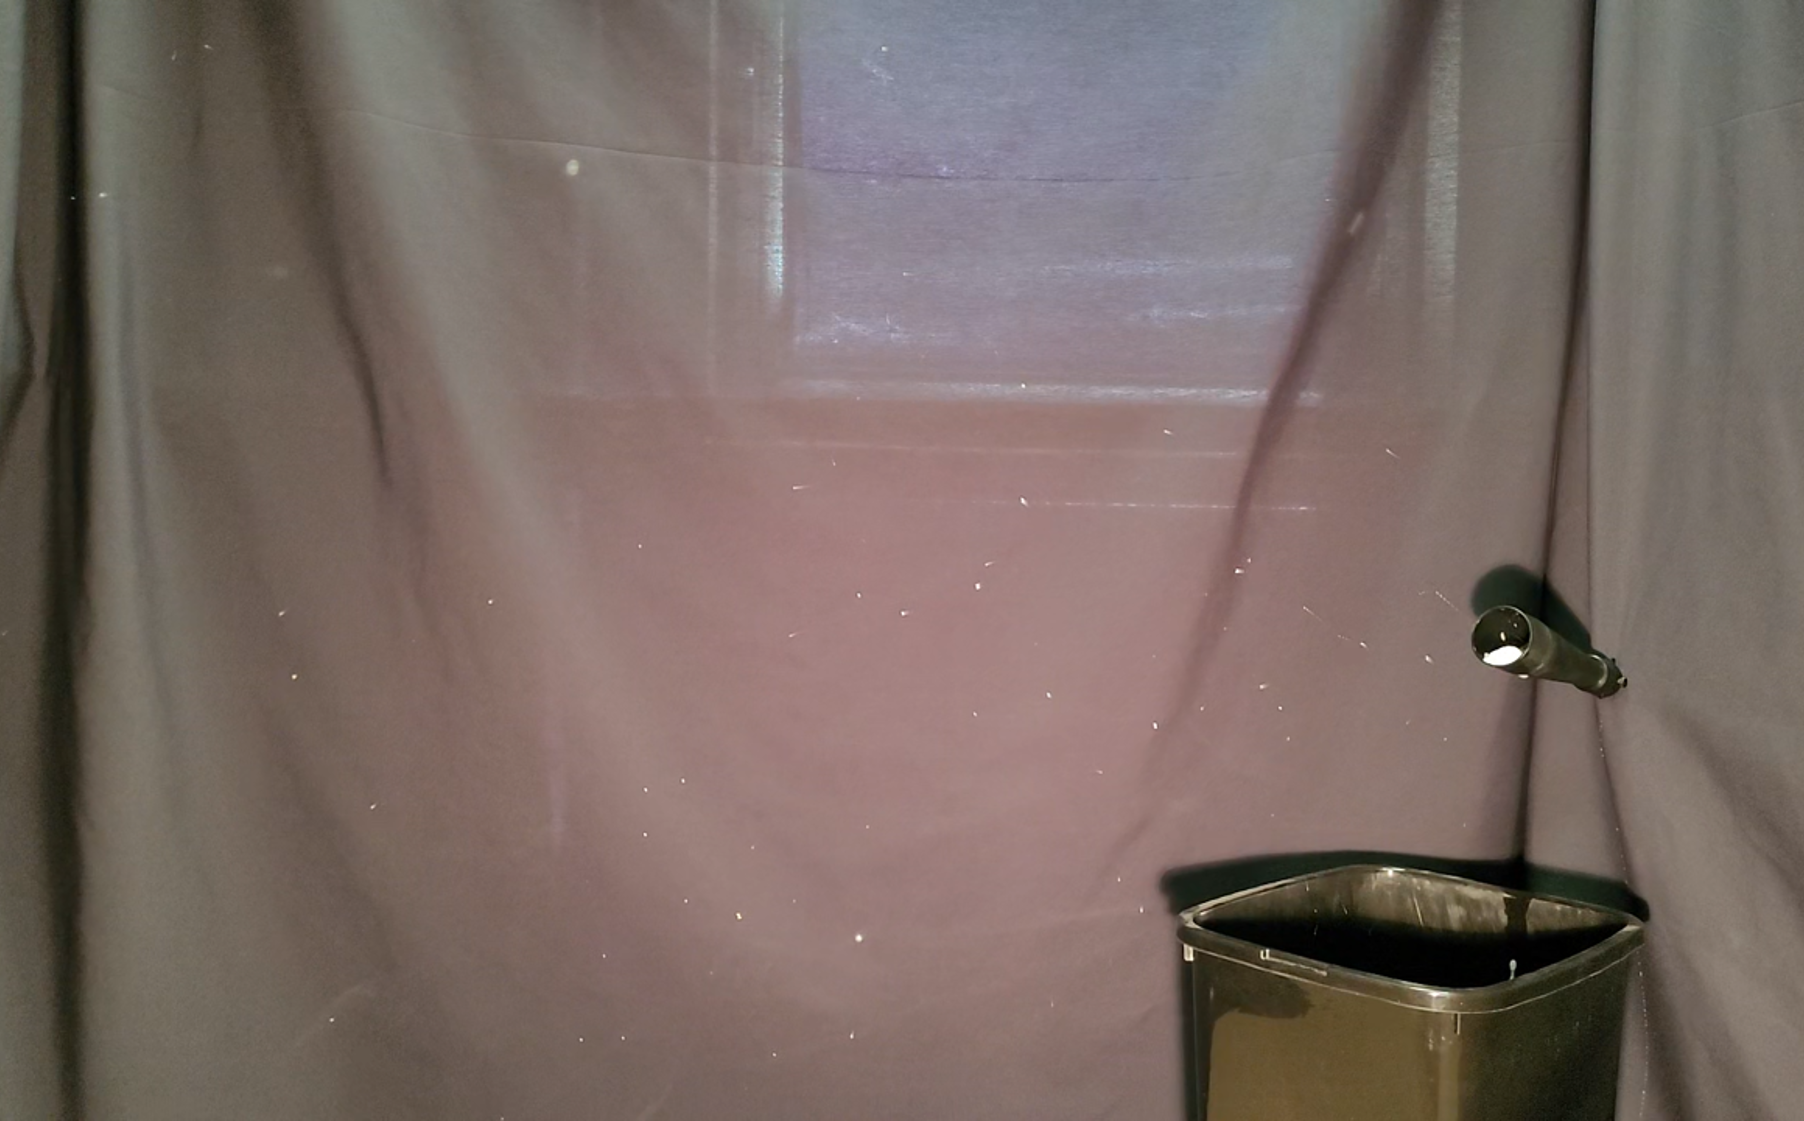
\includegraphics[width=0.9\textwidth]{images/experimental-setup.png}}
	\caption{\centering The experimental setup: the machine in the corner of the room is creating some small bubbles that fill the space}
	\label{fig:experimetal-setup}
\end{figure}

\section{Company objectives}

\subsection{The cameras}

SMA-RTY France~\cite{smarty-website}, the company where I did my internship, has as core business the selling of special-purpose, FPGA-driven cameras.
As such, one of the two tasks contracted to them by the research group was the construction of a specific camera for this purpose: this task was tackled by their internal team of embedded developers.
In the final setup, 3 or 4 cameras were used in a stereoscopic arrangement, as shown in figure~\ref{fig:camera-setup}.

\begin{figure}
	\centerline{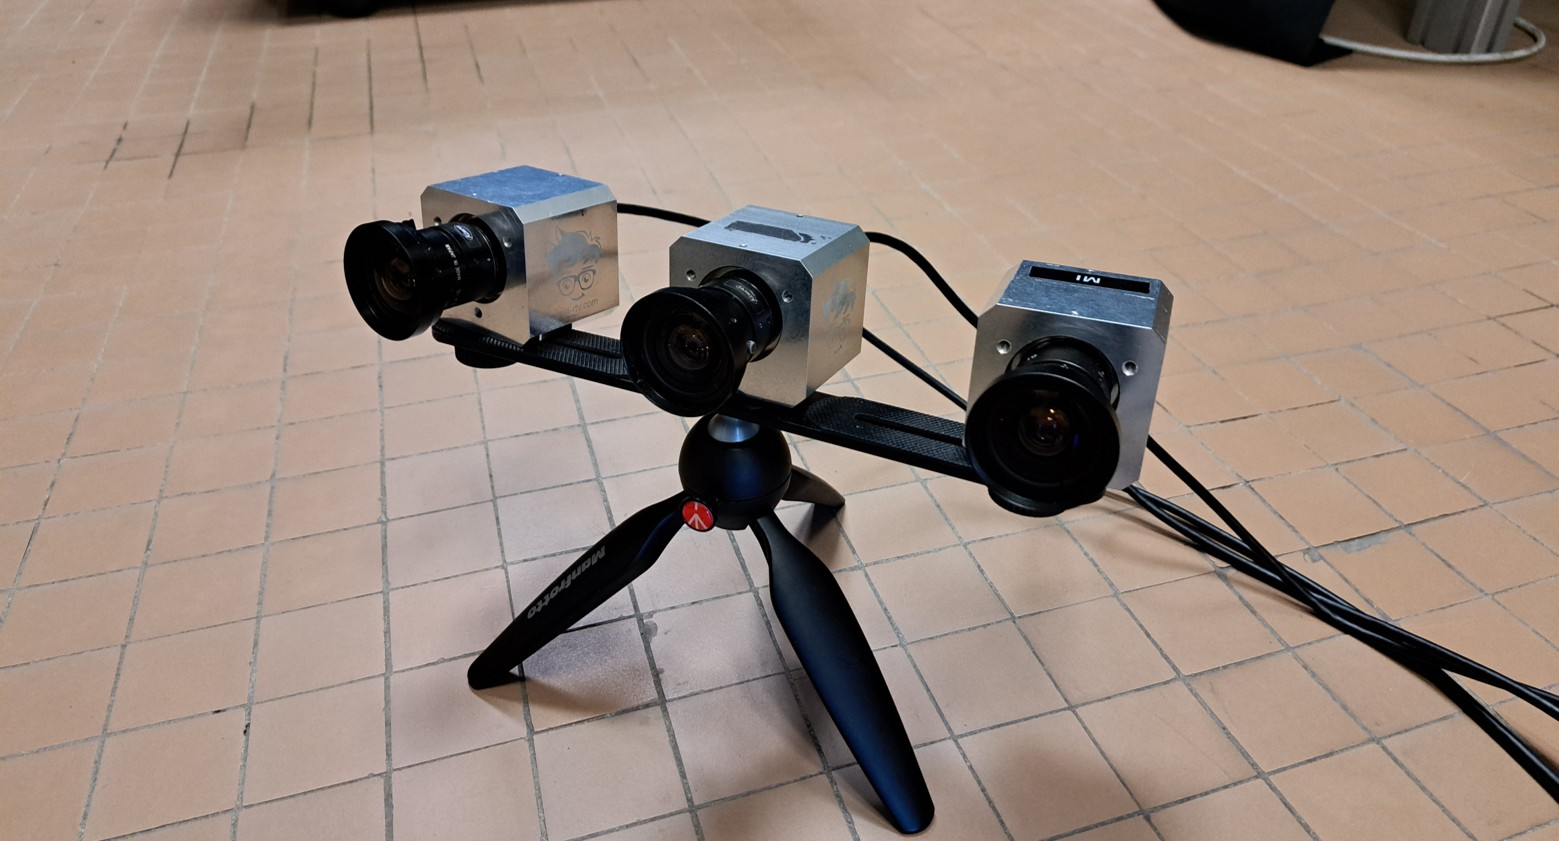
\includegraphics[width=0.9\textwidth]{images/cameras.jpg}}
	\caption{\centering A tripod with 3 SMA-RTY cameras in a stereoscopic arrangement}
	\label{fig:camera-setup}
\end{figure}

\subsection{Reconstruction algorithm acceleration}

The research group internally developed a Matlab tool for analyzing the video footage from an arrangement of 3 cameras, but the processing speed was extremely slow.
As such, they contracted SMA-RTY to create an accelerated version, either by improving the original one, or by creating a totally new script, in whichever programming language was best.
The objective of the acceleration was to have a real-time software, that would be able to process the videos live, with an allowance of some seconds of jitter.
That is, a delay between capturing the frame and outputting the reconstruction was acceptable, as long as it did not increase over time.

SMA-RTY internally started working on this, with an unfinished solution that accelerated the processing to 19 FPS.
This script was already orders of magnitude faster than the original one, but the obtained speed was still less than the target.
On top of this, this unfinished solution was able only to do 2D tracking for each camera, it did not have the 3D reconstruction yet: implementing  it could not have other effects but slow it down.

\section{Thesis objectives}

I was assigned by the SMA-RTY team the task of accelerating the Matlab script for processing the videos.
Originally, the vision was to exploit my CUDA skills to leverage the parallelization of GPUs.
However, as the body of this thesis will make clear, there was not so much parallelization that could be done.
Instead of focusing on ``better'' hardware architectures, the best course of action was indeed to optimize the various software steps.

Therefore, the objective of my thesis became the recreation of the full pipeline, from image capturing to 3d markers rendering.
The main constraint of the result would be the speed, 24 FPS were required at steady-state, while the output quality should be as good as possible.

\chapter{Background knowledge}
\label{chap:background}

\section{Camera calibration}

Camera calibration is the process of estimating the parameters of a vision system.
Three types of calibration parameters exist: distortion, intrinsics and extrinsics.

\subsection[Distortion]{Distortion~\cite{calib-dist}}

\subsubsection{What is distortion}

A camera lens can introduce two types of distortion: radial and tangential.
Radial distortion makes straight lines appear curved in the image, while tangential distortion can make some image parts look closer than they are.
Figure~\ref{fig:distortion} provides a graphical example of both distortion problems.

\begin{figure}
	\centerline{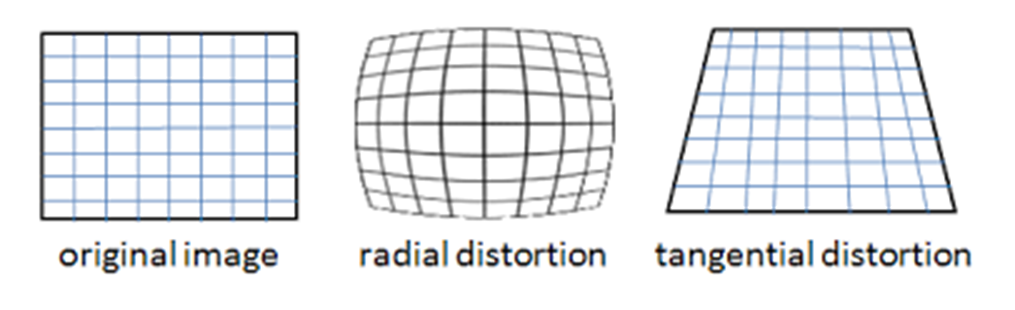
\includegraphics[width=0.6\textwidth]{images/distortion.png}}
	\caption{\centering How radial and tangential distortion affect an image}
	\label{fig:distortion}
\end{figure}

\subsubsection{Mathematical definition}

Given an undistorted point $P=\colvectwo{x}{y}$ (at distance $r$ from the center of the image), a radial distortion will transform it into
\begin{equation}
	P_{dist} = \left( 1 + k_1{\cdot}r^2 + k_2{\cdot}r^4 + k_3{\cdot}r^6 \right) \cdot \colvectwo{x}{y}
\end{equation}
while a tangential distortion would transform it into
\begin{equation}
	P_{dist} = \colvectwo{x+\left[ 2p_1xy + p_2{\cdot}\left( r^2+2x^2 \right) \right]}{y+\left[ 2p_2xy + p_1{\cdot}\left( r^2+2y^2 \right) \right]}
\end{equation}
As such, the full distortion can be described with the vector $\rowvecfive{k_1}{k_2}{p_1}{p_2}{k_3}$

\subsubsection{How to calibrate the parameters}

The estimation of the distortion parameters (among with other parameters) can be computed using \texttt{OpenCV}'s \texttt{calibrateCamera} function.
It requires data extracted from multiple calibration frames, each one with a set of coplanar points.
Each frame must provide the list of pixel coordinates of the points detected in the image.
On top of that, each point must be labeled with a coordinate system local to the plane where the points lay: an example can be a row/column index for a grid-like pattern.

Common calibration patterns are dots (figure~\ref{fig:calibration-planes}.a) or the corners of a chessboard (figure~\ref{fig:calibration-planes}.b).
Often, to help the detection of the chessboard corners, ArUco~\cite{aruco} markers are added in the white cells (figure~\ref{fig:calibration-planes}.c).
This combination of \textbf{ch}essboard and \textbf{ArUco} markers is called \textbf{ChArUco}.

\begin{figure}
	\centering
	\minipage{0.27\textwidth}
	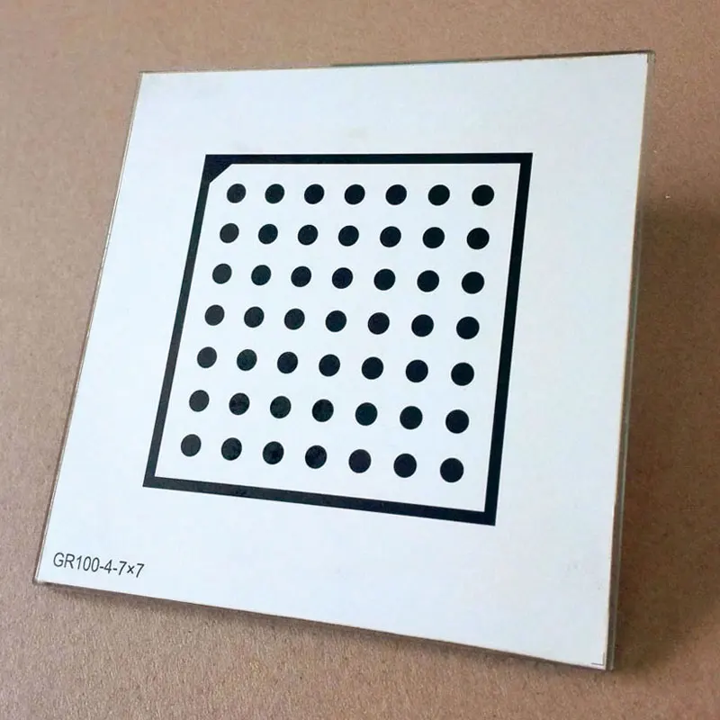
\includegraphics[width=\linewidth]{images/calib-dots.png}
	\caption*{(a)}
	\endminipage\hfill
	\minipage{0.35\textwidth}
	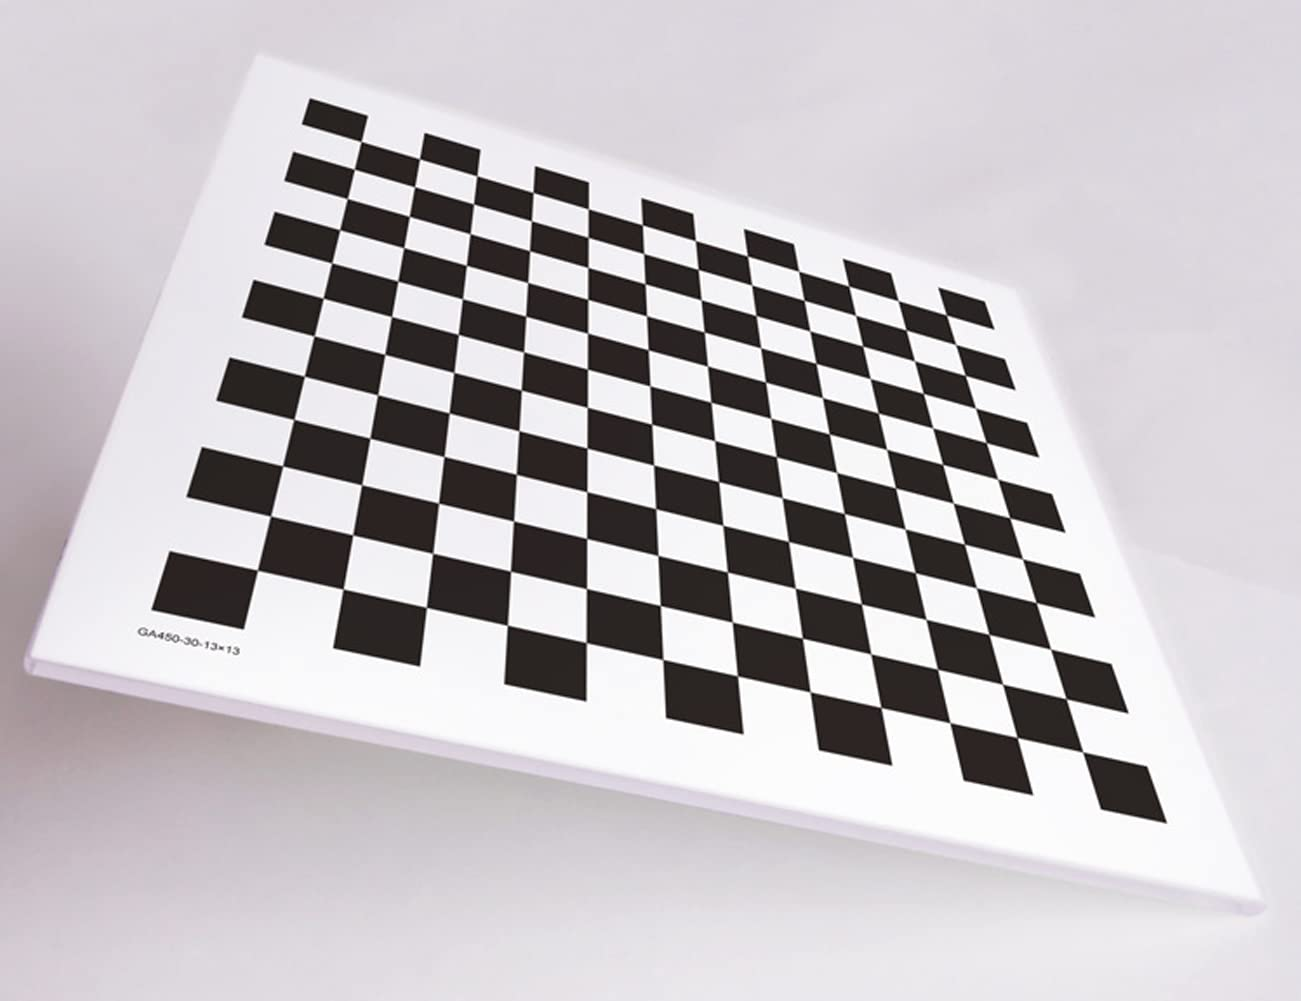
\includegraphics[width=\linewidth]{images/calib-chessb.jpg}
	\caption*{(b)}
	\endminipage\hfill
	\minipage{0.36\textwidth}
	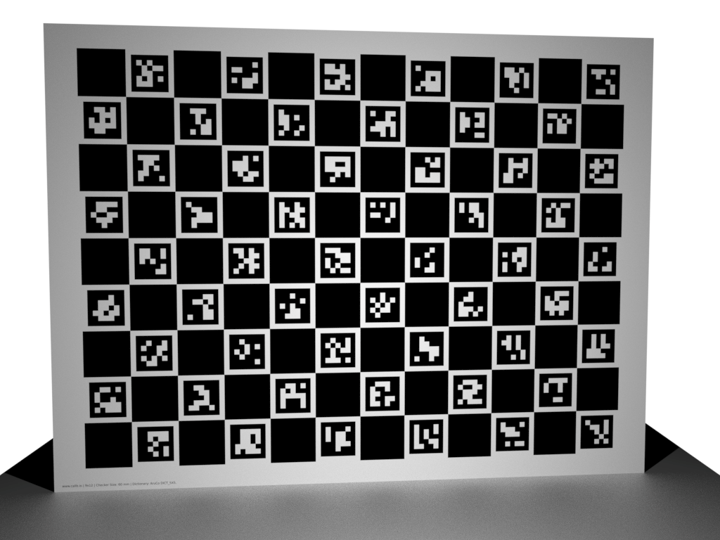
\includegraphics[width=\linewidth]{images/calib-charuco.png}
	\caption*{(c)}
	\endminipage
	\caption{Calibration planes: (a) dots, (b) chessboard, (c) ChArUco.}\label{fig:calibration-planes}
\end{figure}

\subsubsection{How to remove distortion}
Using \texttt{OpenCV}'s \texttt{undistort} function, it is possible to remove the lens distortion.
The result is the image as it would be taken by an ideal camera setup.

\subsection[Intrinsic parameters]{Intrinsic parameters~\cite{calib-intrinsics}}

\subsubsection{What are intrinsic parameters}

The intrinsic parameters describe how the lens and sensor alter the image captured by a single camera.
Using these parameters, it is possible to remove all this distortion, transforming the image into a common frame of reference.
These transforms allow to obtain the same image when two different cameras, with different optics, photograph the same scene.

\subsubsection{Mathematical definition}

Consider a simple scene, with a camera observing a point.
Define a frame of reference centered in the camera.
The point can be described as $R=\rowvecthree{P_x}{P_y}{P_z}^T$.
The camera will project the point onto the image plane, at the homogeneous coordinate $R'=\rowvecthree{P_x'}{P_y'}{1}^T$.
It is possible to show that $P'$ can be written as $P$ transformed by a matrix $K$, called \textbf{intrinsic matrix}: $P' = K{\cdot}P$.

In particular, $K$ is in the form:
\begin{equation}
	K = \begin{bmatrix}
		f_x & s   & x_0 \\
		0   & f_y & y_0 \\
		0   & 0   & 1   \\
	\end{bmatrix}
\end{equation}
where:
\begin{itemize}
	\itemsep 0em
	\item $f_x$ and $f_y$ are the focal lengths in pixels of the optic system. They may differ along the horizontal and vertical direction;
	\item $s$ is the skew, that can be caused by the digitization process;
	\item $x_0$ and $y_0$ are the coordinates of the pixel where the center of projection of the camera stands.
	      % \item $x_0$ and $y_0$ are the horizontal and vertical offset in pixels between the center of projection and the bottom-left corner of the sensor.
\end{itemize}

\subsubsection{How to calibrate the parameters}

The full intrinsic matrix is estimated by the same \texttt{OpenCV} function that evaluates the distortion coefficients.

\subsubsection{How to remove intrinsic parameters}
Using \texttt{OpenCV}'s \texttt{undistort} function, it is possible to remove also the intrinsic parameters.
The result is the image as it would be taken by a camera with $K{=}I_3$.
This enables to compare pixel-wise images captured with different optic and sensor arrangements.

\subsection{Extrinsic parameters}

\subsubsection{What are extrinsic parameters}

The extrinsic parameters describe position and orientation of a camera with respect to a specific frame of reference.
Usually they are not computed when a single camera is present, since it is convenient to assume as frame of reference the position and orientation of the camera.
With multiple cameras, usually one of them is chosen as ``main'', and it acts as the frame of reference for the other cameras.
In this frame of reference it is therefore crucial to understand position and orientation of all the cameras.

Considering camera $A$ as main, the extrinsic parameters of another camera $B$ can be expressed in three different ways:
\begin{itemize}
	\item \textbf{rotation matrix $R$} and \textbf{translation vector $t$}: $R$ describes how to rotate $A$ to be in the same orientation as $B$ (equivalently, how $B$ is rotated in $A$'s frame of reference); $t$ is the versor in $B$'s frame of reference towards the origin (equivalently, $B$ is located in $-Rt$ in the main frame of reference);
	\item \textbf{essential matrix $E$}. Assuming $P_A=\rowvecthree{x_A}{y_A}{1}$ and $P_B=\rowvecthree{x_B}{y_B}{1}$ are the \textit{undistorted} projections of a point $P$ on the two cameras, $E$ is a matrix such that $P_B \cdot E \cdot P_A^T = 0$. $E$ can also be computed as $E = [t]_{\times}R$, where $[t]_{\times}$ is the matrix representation of the cross product of $t$;
	\item \textbf{fundamental matrix $F$}: the definition is the same as $E$'s, but using the points with $K$ still applied (only the distortion has to be removed). If the two cameras have intrinsic matrices $K_A$ and $K_B$, $F$ can be computed as $F = \left(K_A^{-1}\right)^T \cdot E \cdot K_B^T$.
\end{itemize}

\subsubsection{How to calibrate the parameters}

The extrinsic calibration can be obtained from the same data as the intrinsic calibration, provided that the cameras took a picture of the exact same scene (which likely implies that the pictures must be taken at the exact same time instant).
The calibration points detected on both images can be processed by:
\begin{itemize}
	\itemsep 0em
	\item \texttt{OpenCV}'s \texttt{recoverPose} function to obtain $R$ and $t$;
	\item \texttt{OpenCV}'s \texttt{findEssentialMat} function to obtain $E$;
	\item \texttt{OpenCV}'s \texttt{findFundamentalMat} function to obtain $F$.
\end{itemize}

\subsubsection{How to remove extrinsic parameters}

Non-null extrinsic parameters mean that the two images are fundamentally different, therefore it is not possible to remove these parameters.
Instead, these parameters are essential for reconstructing the 3D scene using stereoscopy.

\subsubsection{Definition up to a scale factor}

If everything (objects in the picture, distances between objects and pixel size and focal lenght of the cameras) is scaled by a factor $k$, then the resulting images do not change.
For this reason, the extrinsic parameters can only be defined up to a scale factor.
Most importantly, this affects $t$: it cannot be the vector of the displacement, since the distance is unknown, but it is only the versor of the direction of the displacement.

This makes the reconstruction (stereoscopy) use an arbitrary unit of measurement, which corresponds to the distance between the cameras.
This must be taken into account particularly if there are more than 2 cameras: each camera will have a different distance from the main one, thus having different units of measurement.
The problem can be solved by computing the scaling factor between the units such that the reconstructed calibration points have coherent distance between the different camera couples.
To have a realistic measurement unit, it is also possible to impose this scaling factor in a way that the distance between the reconstructed points is coherent with the real one.

\section{Stereoscopy}

Our brain is able to understand depth by leveraging the fact that we have two eyes in slightly different positions.
This mechanism is called stereoscopy, and it can be used by a computer vision system, provided that it has two or more cameras.

\begin{figure}
	\centerline{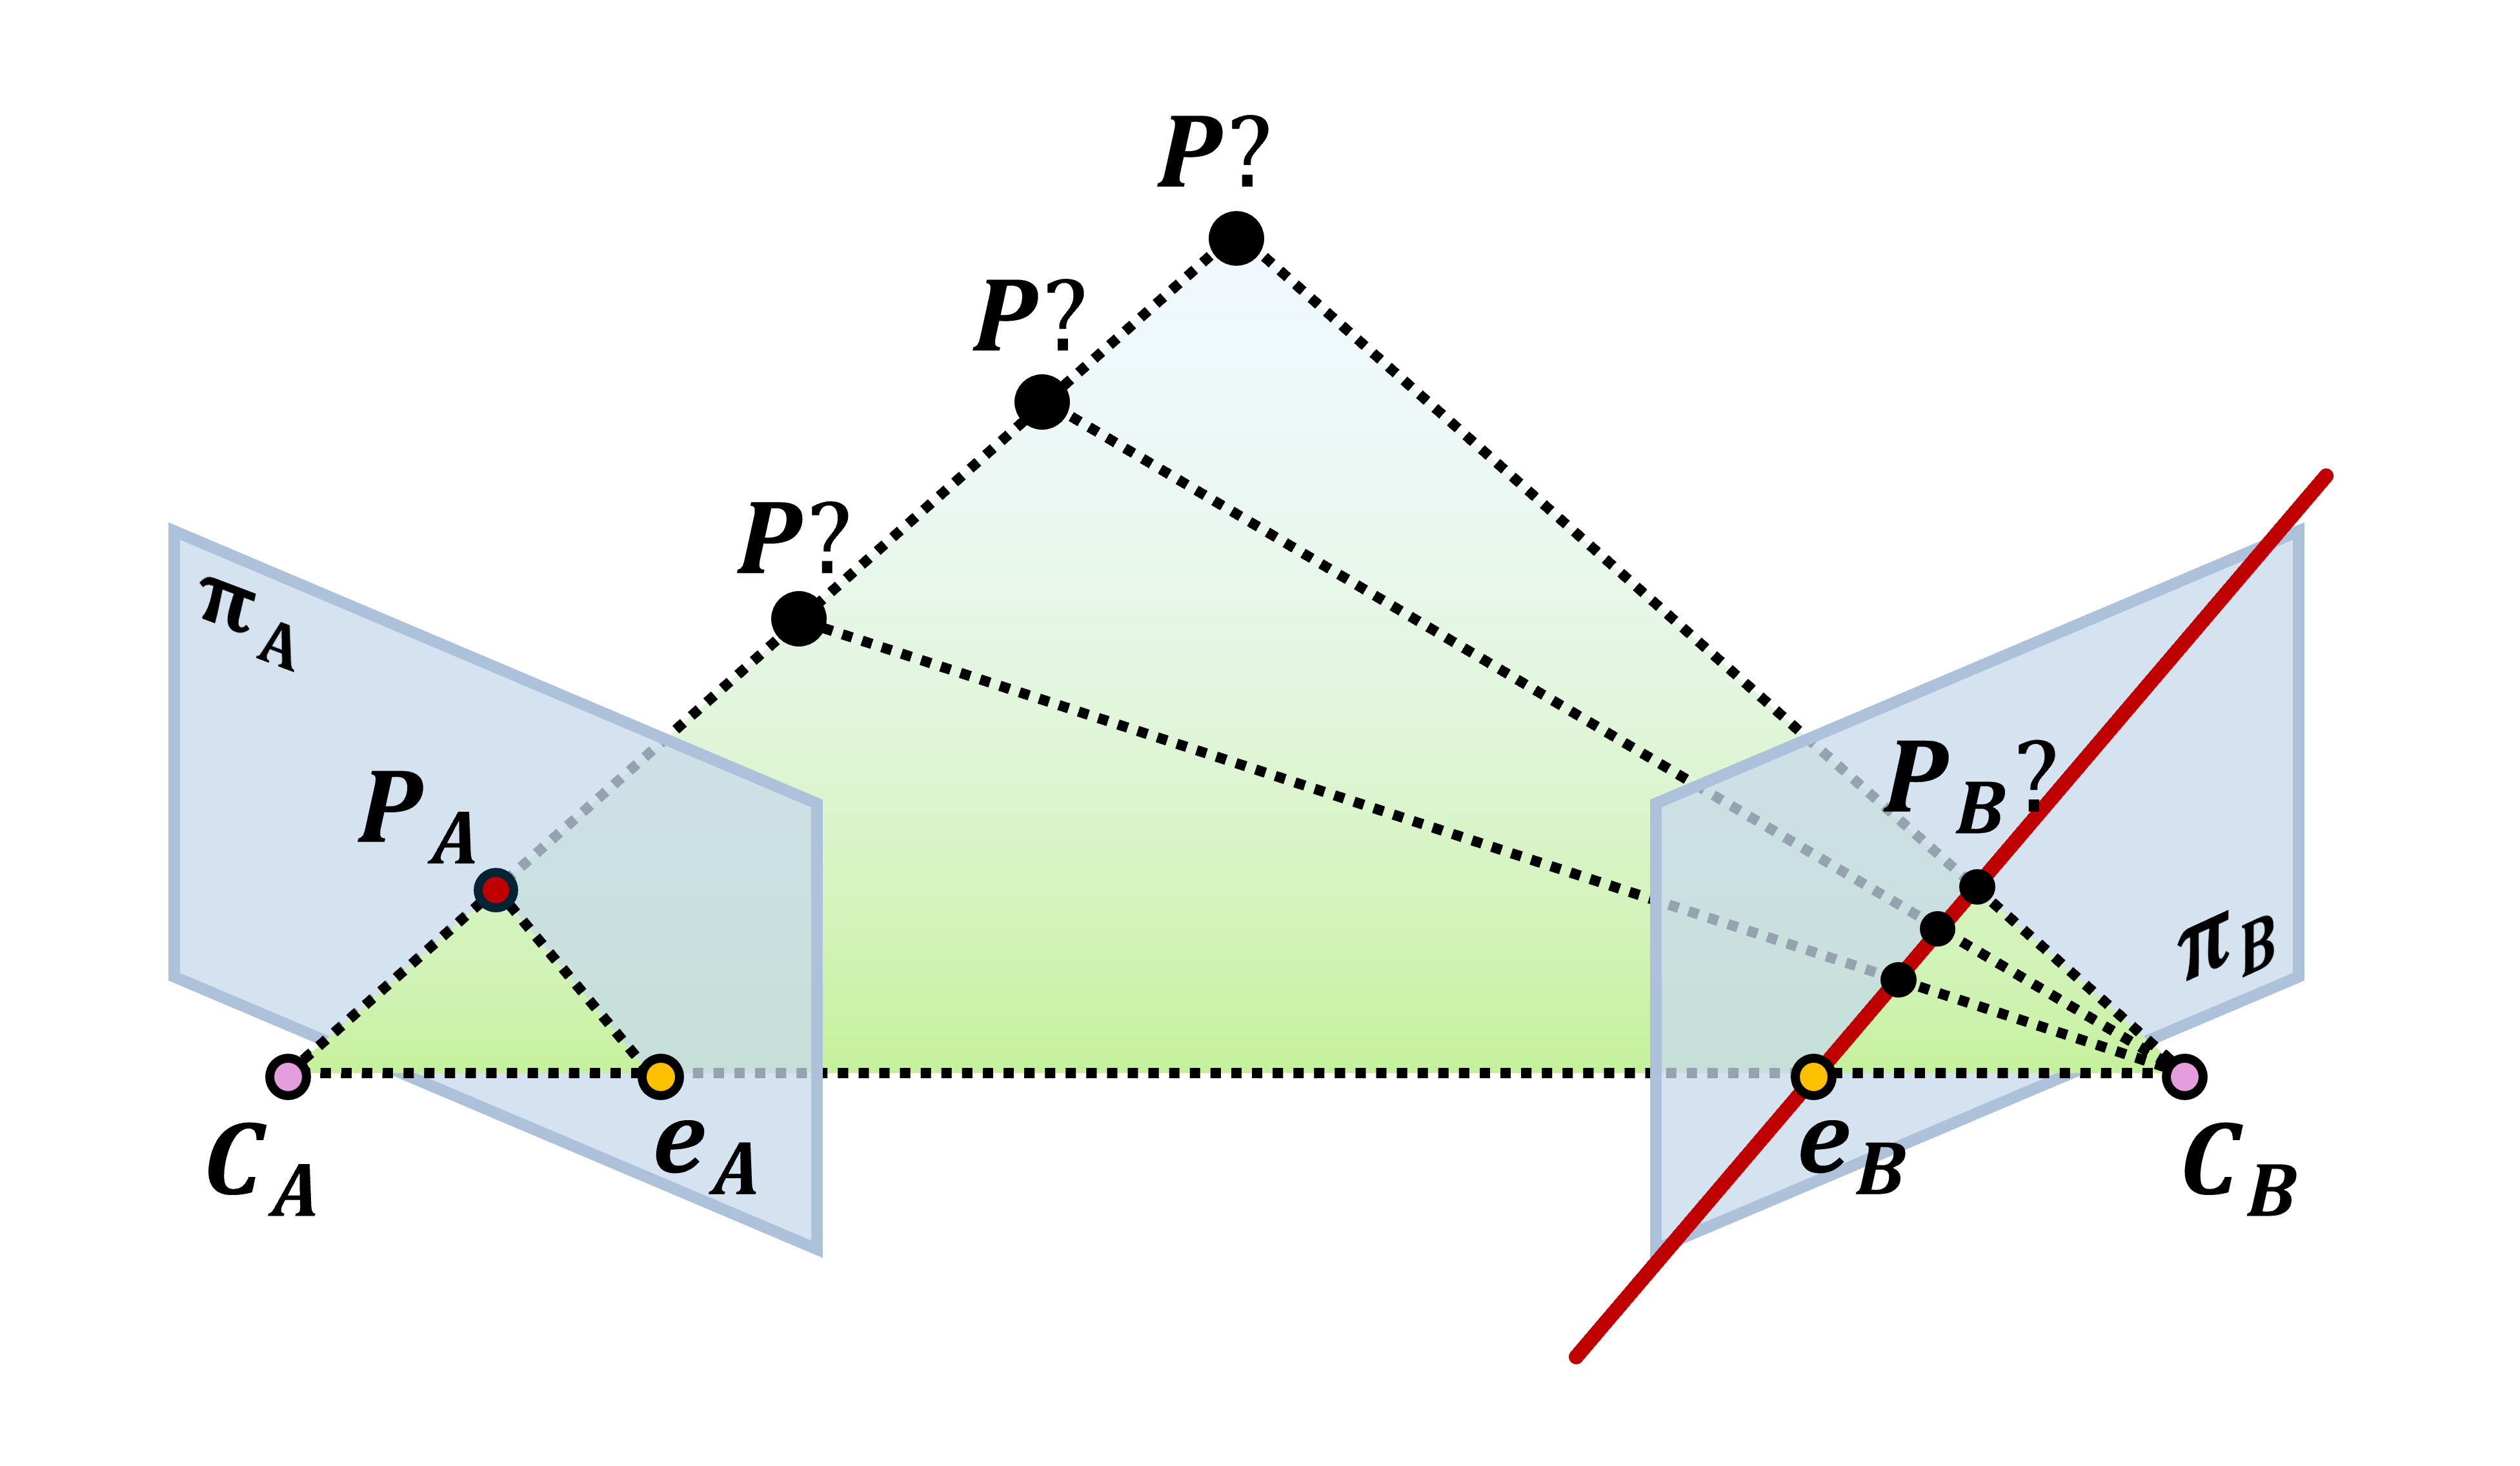
\includegraphics[width=0.8\textwidth]{images/epipolarity.png}}
	\caption{\centering Reprojecting a point from 2D to 3D: it could be anywhere on a specific line}
	\label{fig:epipolarity}
\end{figure}

\subsection{Depth estimation}

Consider a camera $A$, with center of projection $C_A$ and image plane $\pi_A$ (left in figure~\ref{fig:epipolarity}).
If a 3D point $P$ is seen by the camera, in the image plane it will be $P_A = \pi_A \cap \overline{PC_A}$.
From a single camera, it is impossible to reconstruct $P$ from $P_A$: there would be infinitely many possible $P$s, all the points that lie on the extension of $\overline{P_AC_A}$.

If another camera $B$ is available (right in figure~\ref{fig:epipolarity}), and the same point $P$ is projected as $P_B$, then a new information is added: that $P$ will lie on the extension of $\overline{P_BC_B}$.
By intersecting these lines, it is ideally possible to reconstruct the original 3D position of $P$.

In order to do so, the relative position of the cameras needs to be known: all calibration parameters are required.
In particular, the function \texttt{triangulatePoints} from \texttt{OpenCV} is able to reconstruct the 3D positions given the 2D matched observations, the intrinsic and distortion parameters of the two cameras, and the extrinsic matrix of the couple.

\subsection{Epilines}

As stated before, the point $P_A$ could correspond to a full line of 3D points.
When seen by camera $B$ (with a different point of view), this line translates to a 2D line in $\pi_B$ (red in figure~\ref{fig:epipolarity}).
This line is called \textbf{epiline}.

Different points $P_A$ will correspond to different epilines, which however all pass by the \textbf{epipoint} $e_B$.
The epipoint is defined as $e_B = \pi_B \cap \overline{C_AC_B}$.

\subsubsection{Computing the epiline equation}

As explained in the previous section, the essential matrix $E$ is such that $P_B \cdot E \cdot P_A^T = 0$, which is called the \textbf{epipolar constraint}.
If $P_B$ is a generic point on the image, it can be described as $P_B = \rowvecthree{x}{y}{1}$.
The result of $E \cdot P_A^T$ is a $3\times 1$ vector, that can be written without loss of generality as $\rowvecthree{a}{b}{c}^T$.
When all this knowledge is substituted into the epipolar constraint, we obtain the following:
\begin{equation}
	\rowvecthree{x}{y}{1} \cdot E \cdot P_A^T = 0\\
\end{equation}
\begin{equation}
	\rowvecthree{x}{y}{1} \cdot \colvecthree{a}{b}{c} = 0\\
\end{equation}
\begin{equation}
	ax + by + c = 0
\end{equation}
which is the equation of the epiline in $B$'s frame.
% When this information is substituted into the epipolar constraint, the result of the product becomes the equation $ax + by + c = 0$, where $a$, $b$ and $c$ come from $E \cdot P_A^T$.
% Therefore, the epipolar line is 


\subsection{3D matching}

For estimating the depth, \texttt{triangulatePoints} needs matched point.
That is, the $i{-}th$ point provided by camera $A$ and the $i{-}th$ point provided by camera $B$ must be the two projections of the same 3D point.
To perform this matching, traditional stereoscopy follows this procedure:
\begin{enumerate}
	\itemsep 0em
	\item Choose a point in the main image;
	\item Compute the equation of the corresponding epiline;
	\item Consider a patch around the original point;
	\item For each point on the epiline (in the second image), compute the similarity of a patch centered in that point with the original patch;
	\item Select the most similar point as the match;
	\item Compute the 3D coordinate of the point from the obtained match.
\end{enumerate}

\section{Programming languages and libraries}

The particle tracking software that I developed was fully written in Python.
This choice was made considering many reasons, including:
\begin{itemize}
	\itemsep 0em
	\item the extensive quantity of optimized libraries for accomplishing many sub tasks (e.g. \texttt{NumPy});
	\item the simplicity of the syntax, leading to fast development and testing;
	\item the presence of many existing approaches to the problem;
	\item the possibility to run GPU kernels.
\end{itemize}
Initially, there were discussions about testing the different ideas in Python for development speed, to then translate the code into C++, to leverage its faster execution speed.
At the end, the speed of the Python implementation was good enough, so it was kept as the final version, without rewriting.
On top of that, the program relied heavily on advanced \texttt{NumPy} features: a C++ porting would require equivalent manual implementations, thus losing the intrinsic optimizations.

\subsection{NumPy, SciPy, CuPy}

\texttt{NumPy}~\cite{numpy} and \texttt{SciPy}~\cite{scipy} are the classical optimized libraries used for mathematical computations.
\texttt{CuPy}~\cite{cupy} is an alternative to \texttt{SciPy}, that makes use of a GPU to parallelize and accelerate even more the methods.

\subsection{OpenCV}

\texttt{OpenCV}~\cite{opencv} is the most common library used for image handling and computer vision tasks.

\subsection{Numba}

\texttt{Numba}~\cite{numba} is a Just-In-Time compiler for Python: it enables to compile the code instead of interpreting it, improving on Python's infamous slow speed.
On top of this, it enables to write Python kernels that can be compiled into CUDA code, enabling to fully exploit the GPU at the programmer's discretion.

\subsection{Open3D}

\texttt{Open3D}~\cite{open3d} is an open-source library to support the visualization of 3D data.

\subsection{Other libraries}

The libraries \texttt{trackpy}~\cite{trackpy}, \texttt{MyPTV}~\cite{myptv}, \texttt{TracTrac}~\cite{tractrac}, as well as the Matlab tool \texttt{4d-ptv}~\cite{fourdptv}, are different existing solutions for attempting the task. A better analysis follows in the chapters where all the steps are examined.

The library \texttt{PyTorch}~\cite{pytorch}, one of the main pillar of machine learning in Python, is also used in some of the attempts at finding the best solution.

\section{Unity}

TODO REDO

Thanks to my experience in making interactive applications in Unity, I chose this as one of the tools to represent the reconstructed traces.
Its intrinsic 3D render capabilities, combined with its natural interactive nature, made for a perfect tool for this objective.

\chapter{Experimental setup}
\label{chap:experim-setup}

During development, everything was tested on a Jetson Orin Nano, while a final benchmarking was also done ...

\section{Jetson Orin Nano}

The Jetson Orin Nano~\cite{jetson} is a compact but powerful system developed by NVIDIA.
It is powered by a 6-core Arm® Cortex®-A78AE v8.2 64-bit CPU.
It provides an 8GB, LPDDR5 RAM, and accepts an SD card and an external NVMe as mass storage.
It also features a NVIDIA GPU with Ampere architecture, that offers 1024 CUDA cores and 32 tensor cores.
The power consumption can oscillate between 7 and 25W: during our tests, it was always set to maximize performance. 

\section{...}

\chapter{Basic particle tracking pipeline}
\label{chap:basicpipeline}

Commonly, the particle tracking pipeline is split into the following sub tasks:
\begin{enumerate}
	\itemsep 0em
	\item \textit{\textbf{Locate:}} considering each frame of each camera separately, find the pixel coordinates of all the bubbles in the image;
	\item \textit{\textbf{Link:}} consider two consecutive time instants. For each bubble in the first frame, link it to where it moved in the next frame, to form \textbf{tracklets}. This step must take into account potential bubbles that appear or disappear;
	\item \textit{\textbf{3D match:}} consider corresponding frames of the different cameras. For each bubble in one camera, find which is, if any, the corresponding bubble in the other cameras. This information is then used to reconstruct the 3D position of the bubbles;
	\item \textit{\textbf{Visualize:}} display in a suitable way the reconstructed 3D scene on a 2D screen.
\end{enumerate}
In literature, some approaches follow the order 1-2-3-4, performing a camera-wise \textit{Link}.
Some other libraries chose to invert 2 and 3, obtaining a 1-3-2-4 order.
This anticipates the 3D reconstruction before the \textit{Link}, thus performing a single \textit{Link} operation on 3D coordinate, obtaining 3D tracklets.

In the next paragraphs, each step will be analyzed separately.
For each step, I will compare all solutions found in literature among themselves, and with the ones developed by me, to find the overall best one.

\chapter{The \textit{Locate} step}
\label{chap:locate}

\newcommand{\locateimgsize}{0.9\textwidth}

The task of the \textit{Locate} step consists in extracting the positions of the bubbles in pixel coordinates, independently for each frame of each camera.

\section{State of the art}

When searching in literature, many approaches were found to tackle the \textit{Locate} problem.
They were tested and compared with the algorithmic ideas developed within this thesis:
\begin{itemize}
	\itemsep 0em
	\item Section~\ref{sec:locate:trackpy} explores the Trackpy~\cite{trackpy} Python library;
	\item Section~\ref{sec:locate:myptv} explores the MyPTV~\cite{myptv} Python library;
	\item Section~\ref{sec:locate:tractrac} explores the TracTrac~\cite{tractrac} Python program;
	\item Section~\ref{sec:locate:fourdptv} explores the 4d-ptv~\cite{fourdptv} Matlab script.
\end{itemize}

\section{Requirements}

\subsection{Input}
The \textit{Locate} step receives as input the videos captured by the cameras, frame by frame.
The images are pre-processed by an FPGA included in the cameras: the background is removed, and the resulting image is binarized with a threshold, to have distinct white bubbles over a black background.
Figure~\ref{fig:locate:original} depicts an example input frame.

\begin{figure}
	\centerline{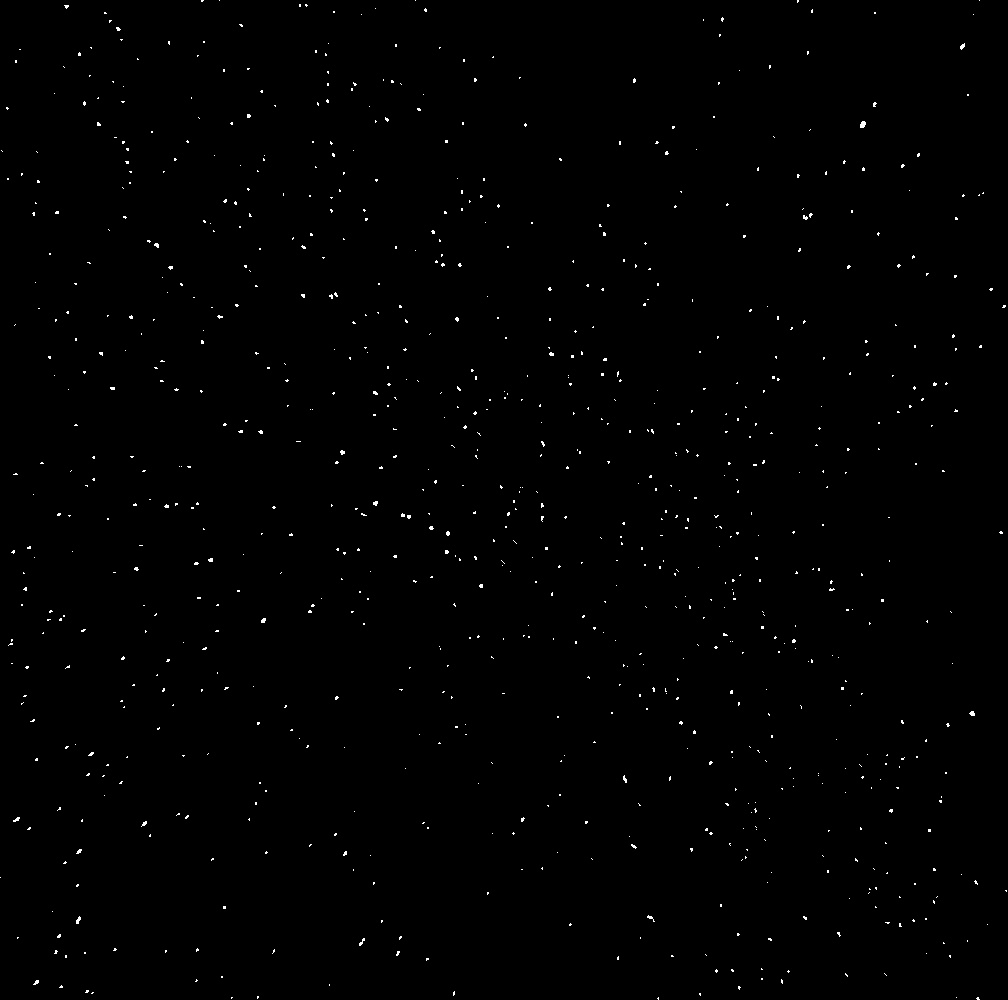
\includegraphics[width=\locateimgsize]{images/locate/_original-frame-full.png}}
	\caption{\centering An example of frame returned by the cameras}
	\label{fig:locate:original}
\end{figure}

\subsection{Output}

The output of the \textit{Locate} step is a couple of \texttt{numpy} arrays.
An array called \texttt{positions} describes the coordinates of each bubble present in a frame. It is a four-dimensional, floating-point array, where \texttt{positions[C][F][B]} describes the $B$-th bubble of the $F$-th frame of camera $C$, in the form of an \texttt{(x, y[, area])} tuple.
Bubbles are ordered in a random, arbitrary way.

Due to \texttt{numpy} limitations, the array is pre-allocated of a fixed size: while the number of cameras is fixed, an upper limit on the number of frames and bubbles must be decided before execution.
Knowing which frames contain meaningful data is trivial, while it is not for the number of bubbles, that can change between frame and frame.
For this reason, a second array was introduced: \texttt{numTracers} is a two-dimensional, integer array.
\texttt{numTracers[C][F]} carries the information of how many tracers are valid inside the $F$-th frame of camera $C$.
The coordinates of the valid tracers will therefore be \texttt{positions[C][F][numTracers[C][F]]}.

\subsection{Speed}

When used on a setup of $N$ cameras with frame rate $f$ each, the \textit{Locate} step would receive $N{\cdot}f$ independent frames each second.
To respect the real-time constraint, the \textit{Locate} step would therefore need to operate at a minimum of $N{\cdot}f$ FPS.

When I did the analysis on the \textit{Locate} step, the plan was to have 3 cameras working at 30 FPS, requiring a 90 FPS \textit{Locate} step.
Later, the cameras turned out to be slower, at 24 FPS, but there were 4: the final \textit{Locate} implementation was able to manage also these 96 FPS.

\subsection{Quality}

Ideally, all tracers should be detected, since errors in the locating process would propagate to future steps:
\begin{itemize}
	\itemsep 0em
	\item \textbf{False positives}: the \textit{3D matching} phase will have more candidates, leading to \textit{possible} wrong reconstructions: the \textit{3D matching} can both choose the correct bubble, or the one added by the error (or another real one);
	\item \textbf{False negatives:} the same bubble in another frame will not have the correct match, leading to \textit{certain} wrong reconstructions.
\end{itemize}
As such, it is better to overpredict (false positives) than to miss bubbles.

It is however to be noted that the most important requirement is the speed: a worse implementation which is speedwise above target should be preferred to a better implementation that does not meet speed requirements.

\section{Approaches}

The following sections describe the many different approaches evaluated for the \textit{Locate} step.
Their speed and quality is compared on a common 1-camera, 100-frame sequence.
Each approach reports an example frame: it is the result of performing the \textit{Locate} on figure~\ref{fig:locate:original-crop}, which itself is a portion of the frame in figure~\ref{fig:locate:original}.

\begin{figure}[H]
	\centerline{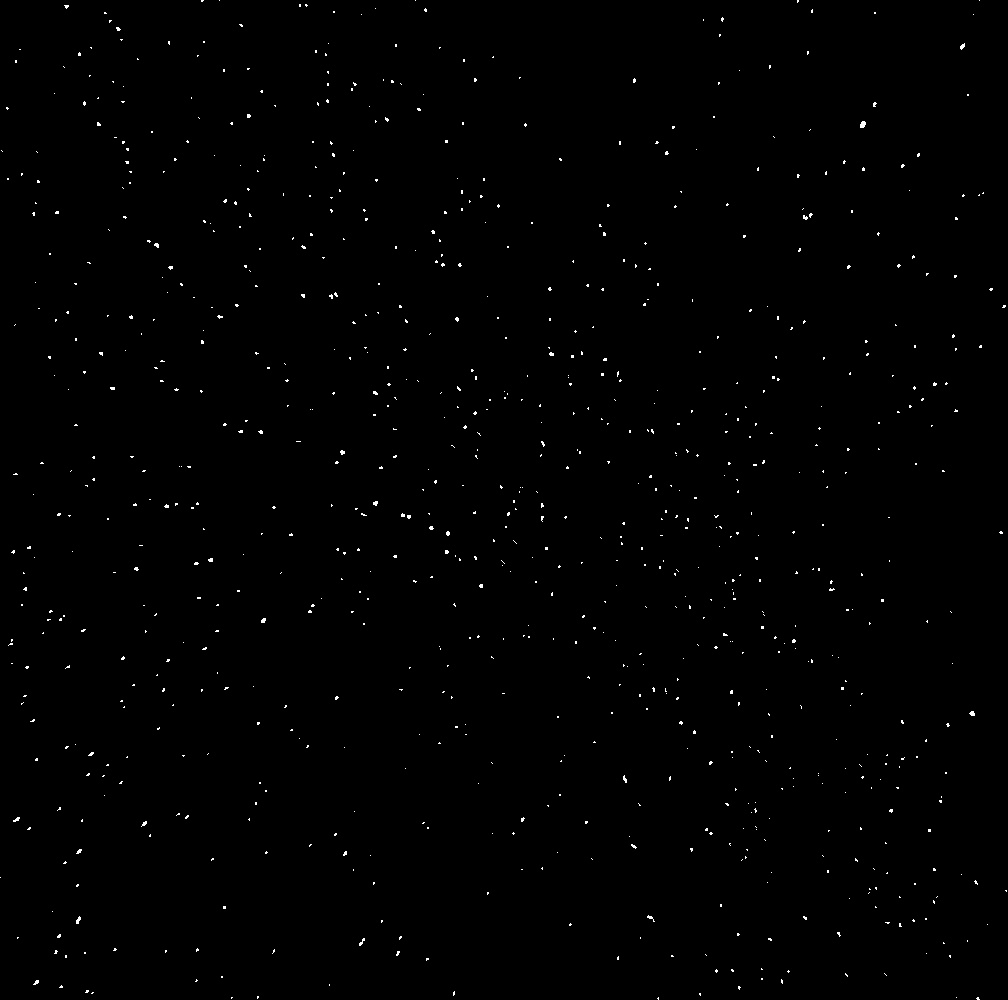
\includegraphics[width=\locateimgsize]{images/locate/_original-frame.png}}
	\caption{\centering An example of frame returned by the cameras}
	\label{fig:locate:original-crop}
\end{figure}


\newpage
\subsection{Trackpy}
\label{sec:locate:trackpy}

Trackpy~\cite{trackpy} is a particle tracking library developed by Soft Matter.
Its \texttt{Locate} function performs the task required, if an extra output format transformation step is applied.

\subsubsection{Algorithm}

As described in the documentation, the \texttt{Locate} function implements the following algorithm:
\begin{enumerate}
	\itemsep 0em
	\item Pre-process the image by performing a band pass and a threshold.
	\item Locate all peaks of brightness, characterize the neighborhoods of the peaks and take only those with given total brightness (``mass'').
	\item Refine the positions of each peak.
\end{enumerate}

\subsubsection{Evaluation}

As displayed in figure~\ref{fig:locate:trackpy}, the algorithm performed well on quality, finding about 85\% of the tracers.
The speed was however extremely low, at just 3 FPS.

\begin{figure}
	\centerline{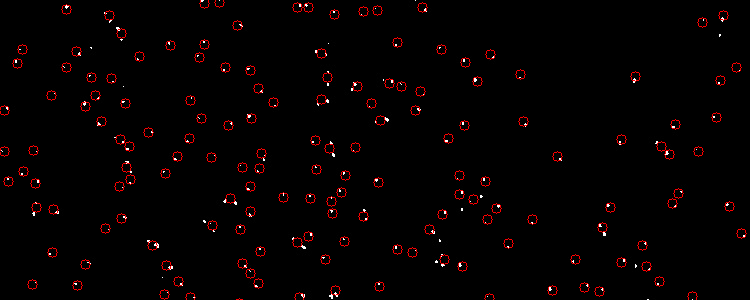
\includegraphics[width=\locateimgsize]{images/locate/trackpy.png}}
	\caption{\centering Trackpy's result}
	\label{fig:locate:trackpy}
\end{figure}
 \newpage
\subsection{Trackpy (CuPy)}

When profiling the Trackpy code, the functions \texttt{fourier\_gaussian}, \texttt{uniform\_filter1d} and \texttt{correlate1d} from \texttt{SciPy} took a considerable amount of time.
For this reason, Trackpy's code was altered to use the \texttt{CuPy} library instead of \texttt{SciPy} for these operations.
This aimed to exploit the GPU for faster computation.

\subsubsection{Algorithm}

The algorithm is the same as Trackpy's, with some extra steps required to transfer the various arrays to/from GPU memory.
These transfers were reduced to the minimum, to reduce the overhead as much as possible.

\subsubsection{Evaluation}

Figure~\ref{fig:locate:trackpy-cupy} shows the result, which for unknown reasons is different than Trackpy's: it lost the offset problem, but the percentage of identified bubbles reduced to 79\%.
Speedwise, the algorithm is slightly faster, running at 7 FPS: still extremely far from the target.

\begin{figure}
	\centerline{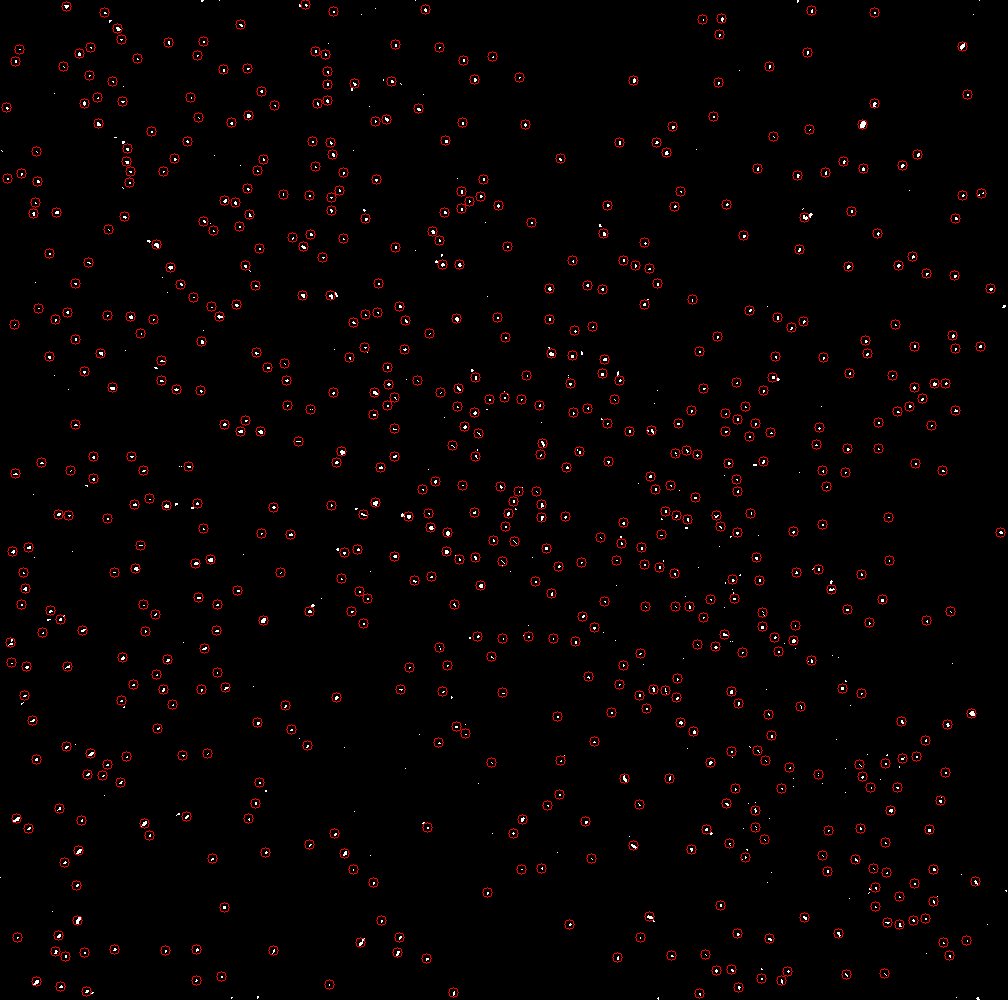
\includegraphics[width=\locateimgsize]{images/locate/cuda-trackpy.png}}
	\caption{\centering Trackpy with CuPy's result}
	\label{fig:locate:trackpy-cupy}
\end{figure}
 \newpage
\subsection{CNN}

The task of \textit{finding the coordinates of the bubbles} can be seen as \textit{for each pixel, check if it is the center of a bubble}.
The task of looking for the same thing across all pixels of an image is the foundation of image convolution and convolutional layers in neural network.
As such, a SAME CONV neural layer was proposed, with a kernel size big enough for containing a full bubble.
The CNN would transform the input image into a binary image, where ``on'' pixels would represent bubble centers.

\subsubsection{Algorithm}

\begin{itemize}
	\itemsep 0em
	\item Initially, the single-layer CNN evaluates the image, to find centroids of the bubbles;
	\item At a second stage, a loop would collect all the ``on'' pixels of the image into a list of coordinates.
\end{itemize}

\subsubsection{Evaluation}

Initially, only a feasibility study was performed: the CNN was trained with just a single epoch of 8 images, to evaluate if the inference speed was good enough to justify a longer training.
The result shown in figure~\ref{fig:locate:cnn} is promising for the little training performed, but it clearly needs more refinement.

Most importantly, the speed was much greater than the previous ones, at 55 FPS, but still far from the target.
As such, further approaches would be evaluated before performing a deeper training, to investigate if a greater speed was achievable.

\begin{figure}
	\centerline{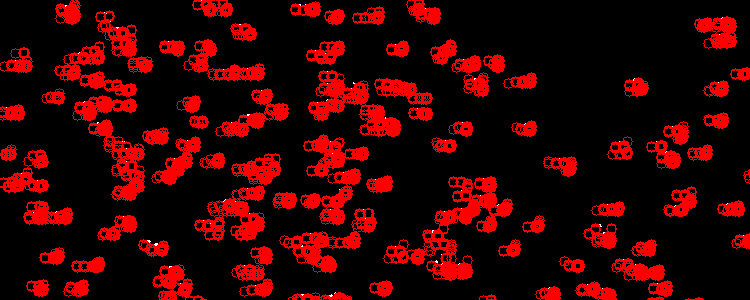
\includegraphics[width=\locateimgsize]{images/locate/cnn.png}}
	\caption{\centering The CNN's result}
	\label{fig:locate:cnn}
\end{figure}
 \newpage
\subsection{Torch.unfold concept}
\label{sec:locate:torchunfold}

The \texttt{unfold} function from \texttt{PyTorch} takes an image, and breaks it into either disjoint or partially overlapping tiles.
The idea is to use a divide and conquer approach, where the full image is split into smaller images, hopefully making it faster.


\subsubsection{Algorithm}

The overall algorithm divides the image into patches, to then process each one separately.
Different tile sizes were compared, to find the best, if any.

\subsubsection{Evaluation}

As visible in table~\ref{tab:torch.unfold}, having smaller patches increases the time required to perform the overall \locate*.
This is likely due to the overlap between patches.
The overlap is however necessary, to avoid bubbles split across patches to be considered as separate.

\begin{table}[ht]
	\centering
	\def\arraystretch{2}
	\begin{tabularx}{\linewidth}{
		|>{\arraybackslash}p{.2\linewidth}
		|>{\centering\arraybackslash}X
		|>{\centering\arraybackslash}X
		|>{\centering\arraybackslash}X
		|>{\centering\arraybackslash}X
		|>{\centering\arraybackslash}X
		|>{\centering\arraybackslash}X|
		}
		\hline
		\textbf{Patch size [px]} & 501{$\times$}501 & 101{$\times$}101 & 51{$\times$}51 & 25{$\times$}25 & 15{$\times$}15 & 11{$\times$}11 \\ \hline
		\textbf{Time [s]}        & 1.57             & 3.90             & 7.02           & 18.22          & 49.65          & 96.59          \\ \hline
	\end{tabularx}
	\def\arraystretch{1}
	\caption{Time required to process 1 frame with different patch sizes}
	\label{tab:torch.unfold}
\end{table}
 \newpage
\subsection{MyPTV}
\label{sec:locate:myptv}

...

\subsubsection{Algorithm}

...

\subsubsection{Evaluation}

...

% \begin{figure}
% 	\centerline{\includegraphics[width=\locateimgsize]{images/locate/...}}
% 	\caption{\centering ...'s result}
% 	\label{fig:locate:...}
% \end{figure}
 \newpage
\subsection{GPU algorithm}

...

\subsubsection{Algorithm}

...

\subsubsection{Evaluation}

...

% \begin{figure}
% 	\centerline{\includegraphics[width=\locateimgsize]{images/locate/...}}
% 	\caption{\centering ...'s result}
% 	\label{fig:locate:...}
% \end{figure}
 \newpage
\subsection{Iterative concept}

All the approaches generally consider each frame to be independent, not related to the other ones.
This is sometimes required, since for the first processed frame no information is available.
However, since bubbles do not move much between frames, for subsequent frames an algorithm can reduce the searching window around where the bubbles could potentially be.
This knowledge can reduce the searching space for these following frames.

While the idea of searching in smaller patches may seem silly due to the results discussed in section~\ref{sec:locate:torchunfold}, here the situation is different.
Instead of searching in smaller, but meaningless and overlapping regions, this concept uses meaningful and more sparse patches.

\subsubsection{Algorithm}

The algorithm stores position, velocity and acceleration of the previously found bubbles into a list.
Velocity and acceleration are computed from the last and last two positions, respectively.
If such information is not available, the values are considered to be 0.

The different frames are processed differently, based on their index:
\begin{enumerate}
	\itemsep 0em
	\item First frame:
	      \begin{enumerate}
		      \itemsep 0em
		      \item Perform a full frame \textit{Locate};
		      \item Add all the bubbles into the (previously empty) list.
	      \end{enumerate}
	\item All other frames:
	      \begin{enumerate}
		      \itemsep 0em
		      \item Consider the bubbles currently in the list;
		      \item Estimate their future position based on the current velocity and acceleration;
		      \item In a patch around the predicted position, perform a \textit{Locate};
		      \item If the bubble is found, update its trajectory;
		      \item Otherwhise, if a bubble is lost for some frames, remove it from the list.
	      \end{enumerate}
	\item Every $N$ frames:
	      \begin{enumerate}
		      \itemsep 0em
		      \item Update the existing bubbles according to step 2;
		      \item Perform a full frame \textit{Locate}, to find potential bubbles that appeared in the last $N$ frames;
		      \item Add to the list the bubbles that were found by this full frame \textit{Locate}, and are not yet present in the list.
	      \end{enumerate}
\end{enumerate}

This concept is a ``meta-algorithm'', in the sense that it relies on another \textit{Locate} algorithm as a backend.
For the evaluation, multiple underying algorithm was chosen as backend.

\subsubsection{Evaluation}

Both the qualty and the speed of the meta-algorithm were worse than the original algorithm.
For example, when using the Hough algorithm (see section~\ref{sec:locate:hough}), the quality was reduced from 84\% to 43\%, and the speed from 55 to 15 FPS.

This meant that the divide and conquer approach was not advantageous, even if the tiles were meaningful.

\begin{figure}
	\centerline{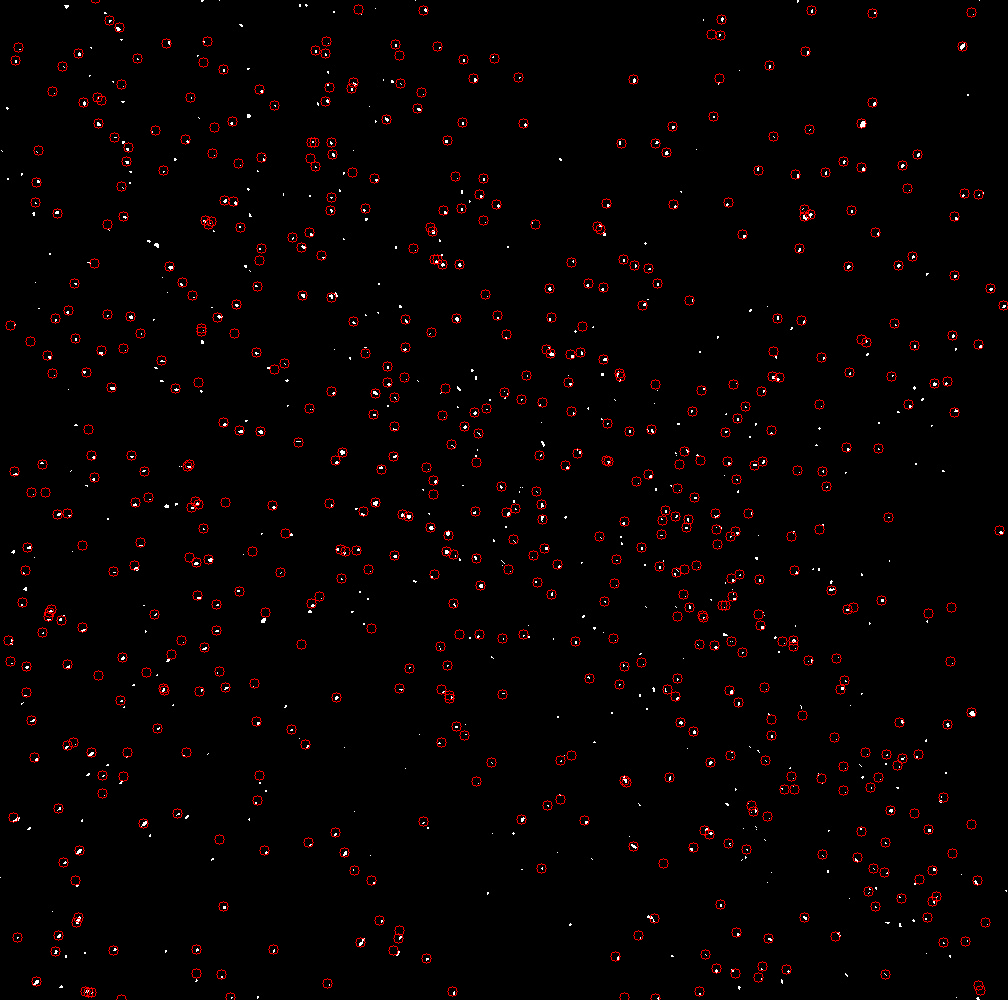
\includegraphics[width=\locateimgsize]{images/locate/iterative-Hough.png}}
	\caption{\centering Iterative concept with Hough backend's result}
	\label{fig:locate:...}
\end{figure}
 \newpage
\subsection{TracTrac}
\label{sec:locate:tractrac}

...

\subsubsection{Algorithm}

...

\subsubsection{Evaluation}

...

% \begin{figure}
% 	\centerline{\includegraphics[width=\locateimgsize]{images/locate/...}}
% 	\caption{\centering ...'s result}
% 	\label{fig:locate:...}
% \end{figure}
 \newpage
\subsection{Hough transform}
\label{sec:locate:hough}

...

\subsubsection{Algorithm}

...

\subsubsection{Evaluation}

...

% \begin{figure}
% 	\centerline{\includegraphics[width=\locateimgsize]{images/locate/...}}
% 	\caption{\centering ...'s result}
% 	\label{fig:locate:...}
% \end{figure}
 \newpage
\subsection{GPU Hough}

The Hough algorithm operates iterating over all pixels of an image.
As such, a new approach was developed, where this loop is replaced by a parallel GPU kernel call.

\subsubsection{Algorithm}

The general algorithm is the same as presented in~\ref{sec:locate:hough}, with all steps executed in GPU.
In particular:
\begin{itemize}
	\itemsep 0em
	\item Step 1 is performed by a kernel, with synchronization after it;
	\item Step 2 is executed by a separate kernel, with synchronization after;
	\item Steps 3 and 4 are run by a unique kernel, that executes non-max suppression on its own pixel, and if it not suppressed, uses atomic methods to add the pixel as coordinate center.
\end{itemize}
On top of the pixels of each frame, also the frames themselves were processed in parallel.

\subsubsection{Evaluation}

The performance of this approach is worse than the CPU Hough transform, both in quality and speed: the algorithm only identifies about 65\% of the bubbles (as visible in figure~\ref{fig:locate:gpu-hough}), running at 17 FPS.

\begin{figure}
	\centerline{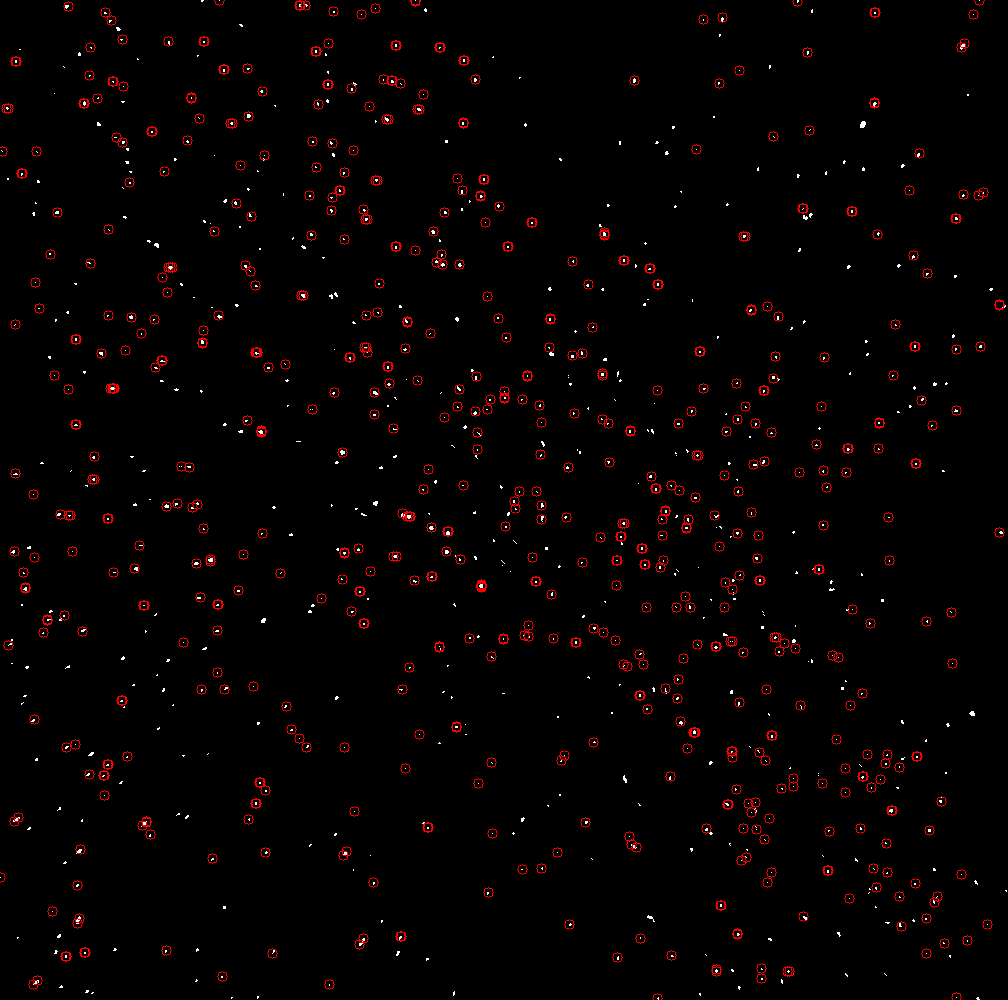
\includegraphics[width=\locateimgsize]{images/locate/my-hough-transform.png}}
	\caption{\centering GPU Hough's result}
	\label{fig:locate:gpu-hough}
\end{figure}
 \newpage
\subsection{4d-ptv}

...

\subsubsection{Algorithm}

...

\subsubsection{Evaluation}

...

% \begin{figure}
% 	\centerline{\includegraphics[width=\locateimgsize]{images/locate/...}}
% 	\caption{\centering ...'s result}
% 	\label{fig:locate:...}
% \end{figure}
 \newpage
\subsection{Image moments}

Thanks the preprocessing done by FPGA, the \locate* task is equivalent to finding homogeneous regions of white pixels on top of a black background.
This task is implemented by the function \texttt{FindContours}~\cite{findcontours} from \texttt{OpenCV}, that finds a rectangular bounding box around pixels with the same intensity.
The precise coordinates of the bubble centroid can be found by computing the centroid (the image moments, see section~\ref{sec:backgr:moments}) of each bounding box.

\subsubsection{Algorithm}

\begin{enumerate}
	\itemsep 0em
	\item Through \texttt{OpenCV}'s \texttt{FindContours}, find all the bubbles for a given frame;
	\item For each region in the output:
	      \begin{enumerate}
		      \item Compute the image moments with \texttt{OpenCV}'s \texttt{moments} function;
		      \item Use the moments of order 0 and 1 to compute the centroids;
		      \item Add the coordinates to the output list.
	      \end{enumerate}
\end{enumerate}

\subsubsection{Evaluation}

As visible in figure~\ref{fig:locate:moments}, the result quality is almost perfect, finding about 99\% of bubbles.
The speed of 67 FPS is extremely good as well, while still being lower than the target.

\begin{figure}
	\centerline{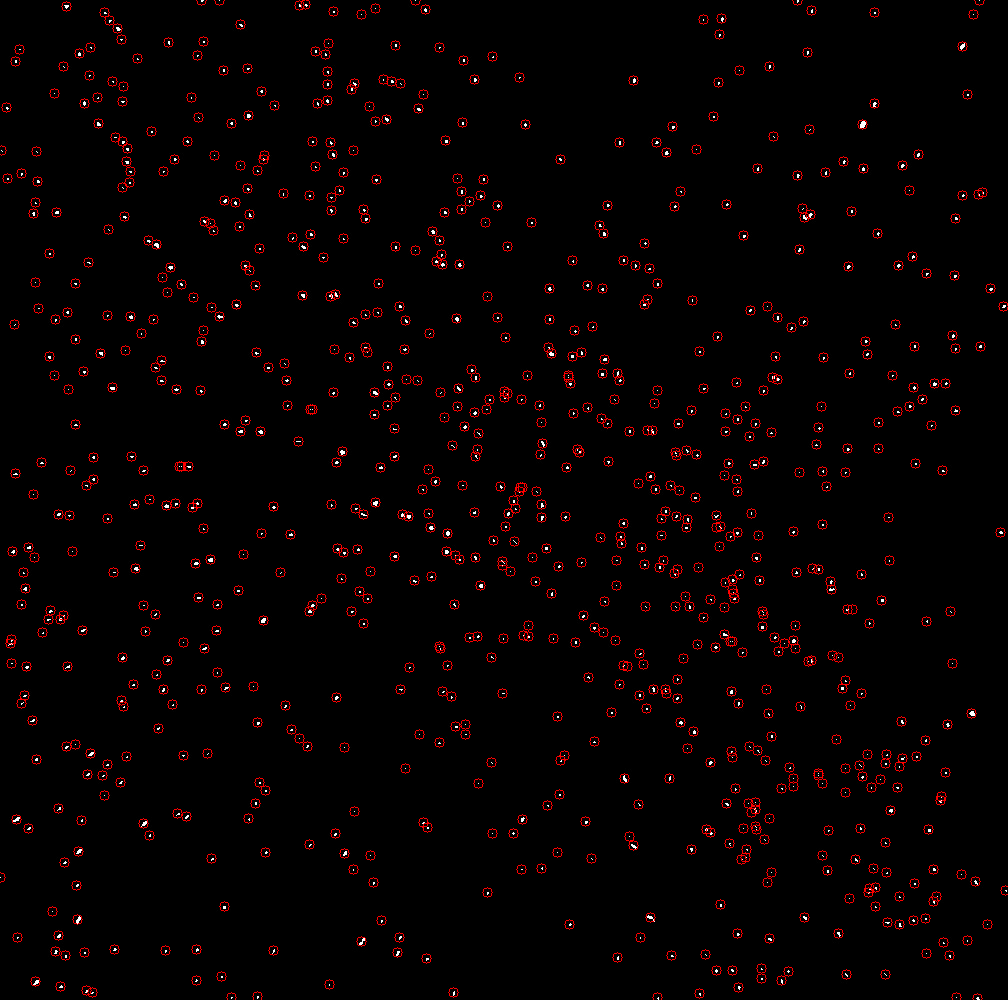
\includegraphics[width=\locateimgsize]{images/locate/opencv moments.png}}
	\caption{\centering Image moments's result}
	\label{fig:locate:moments}
\end{figure}
 \newpage
\subsection{GPU moments}
\label{sec:locate:gpu-moments}

From the previous approach, it was noticed that computing the moments on the different bubbles was a highly parallelizable task.
In fact, the same \texttt{moments} function was called for each bubble found by \texttt{FindContours}.

On top of that, the \texttt{moments} function used to compute moments up to order 3 (for a total of 24 moments), while only moments of order 0 and 1 were used.
As such, a tailored, GPU implementation was created to compute the centroids of the bubbles.
The resulting implementation was also extended to process contours of multiple cameras at the same time,  as well as considering more frames of the same camera in a batch.

\subsubsection{Algorithm}

\begin{enumerate}
	\itemsep 0em
	\item Through \texttt{OpenCV}'s \texttt{FindContours}, find all the bubbles for a given frame;
	\item Find the largest contour among them (this allows all GPU threads to work on the same data size, to avoid diversions);
	\item For each contour found, a GPU thread runs the following kernel:
	      \begin{enumerate}
		      \item Iterate over all pixels, accumulating $M_{00}$, $M_{01}$ and $M_{10}$;
		      \item Use the moments to compute the centroids;
		      \item Add the coordinates to the output list.
	      \end{enumerate}
\end{enumerate}

\subsubsection{Evaluation}

Since the algorithm the exact porting of the corresponding CPU algorithm, the output is the same (figure~\ref{fig:locate:moments}, 99\% of bubbles found).

For the speed evaluation, some tests were conducted to find the best, if any, batch size.
Figure~\ref{fig:locate:moments-cpu-vs-gpu} compares the speed of the CPU algorithm to the speed of the GPU algorithm, with respect to the total number of frames the GPU algorithm processes together.
In particular, this number corresponds to the product between the number of cameras and the batch size per camera.
It is visible that the GPU algorithm is faster, provided that at least 5 frames are processed concurrently, while reaching plateau performance when 10 frames are considered at each iteration.
For the final evaluation, we chose a batch size of 20 per camera, leading to 80 frames processed at the same time by the GPU.

While increasing this batch size adds a delay on the output, this delay only produces a one-time latency, not accumulating over time.
This is acceptable according to the project requirements, which allow for some processing latency, while requiring real-time regime speed.

The maximum speed achieved for this approach was 73 FPS, making this the fastest approach among all, but still not fully reaching the real-time target.

\begin{figure}
	\centerline{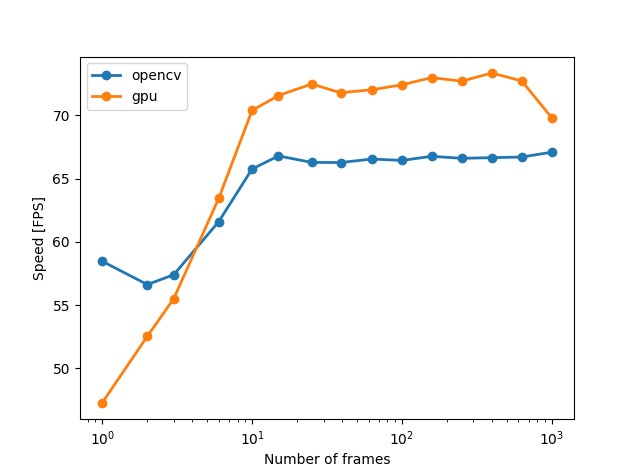
\includegraphics[width=.6\textwidth]{images/moments_opencv_vs_gpu.png}}
	\caption{\centering Comparing speed between CPU and GPU Image Moments algorithms with respect to number of frames processed}
	\label{fig:locate:moments-cpu-vs-gpu}
\end{figure}
 \newpage

\section{Final choice}

All the previously described approaches were compared among each other and with the target speed.
As visible in figure~\ref{fig:locate:speed}, none of the approaches was able to reach the target 90 FPS.
Since no other approach or idea was available, the fastest algorithm (GPU moments, described in section~\ref{sec:locate:gpu-moments}) was chosen.
Incidentally, the selected algorithm was also one of the best in terms of output quality.

\begin{figure}
	\centerline{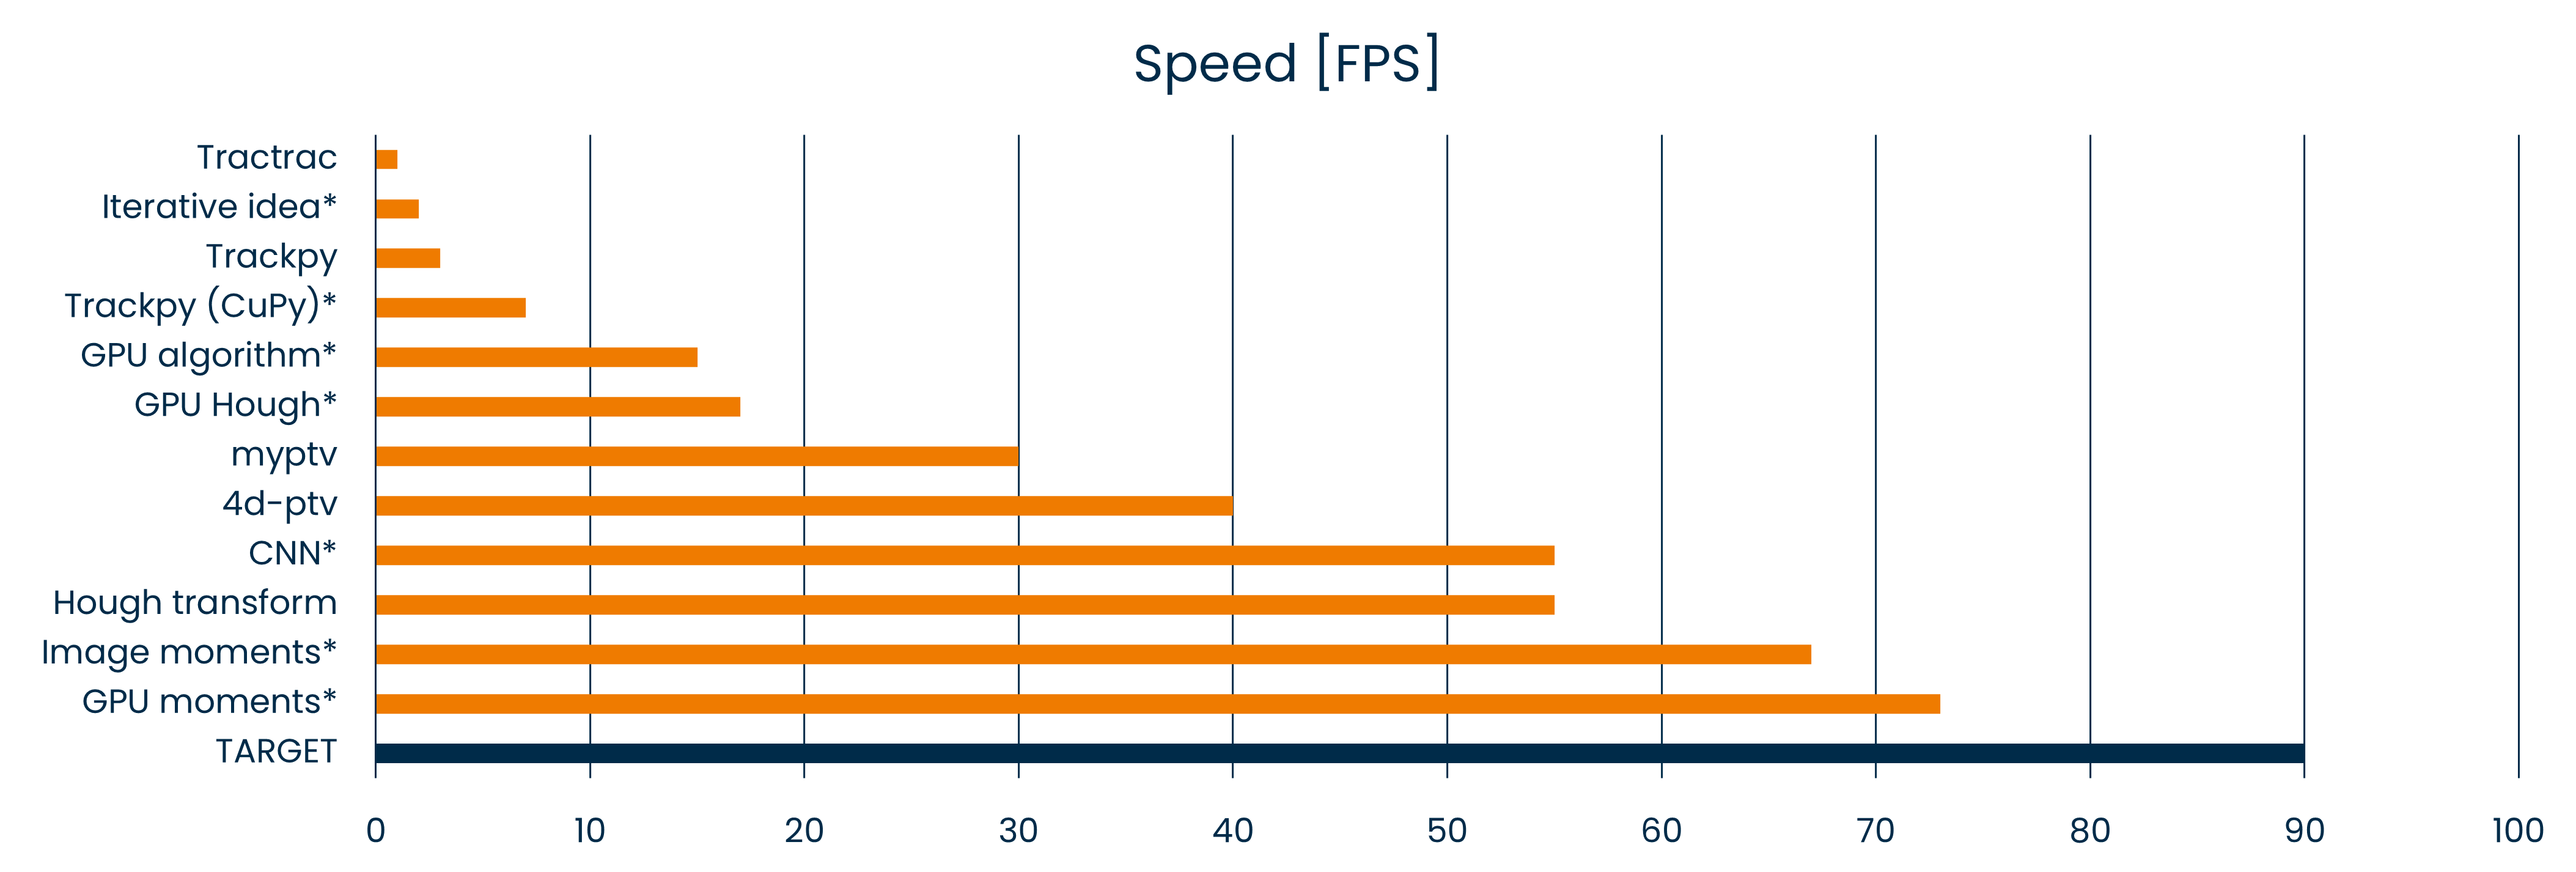
\includegraphics[width=\textwidth]{images/locate-speed-comparison.png}}
	\caption{\centering Performance evaluation of different approaches for the \textit{Locate} step.}
	\label{fig:locate:speed}
\end{figure}

To compare the different approaches with each other, some modifications were required to ensure consistency, for simpler comparison.
After choosing the final algorithm, it was implemented again from scratch, in order to make it as fast as possible, with no overhead.
This resulted in a decent speedup, which enabled the algorithm to execute at 102 FPS, faster than the target speed, as visible in figure~\ref{fig:locate:speed-cleansheet}.

\begin{figure}
	\centerline{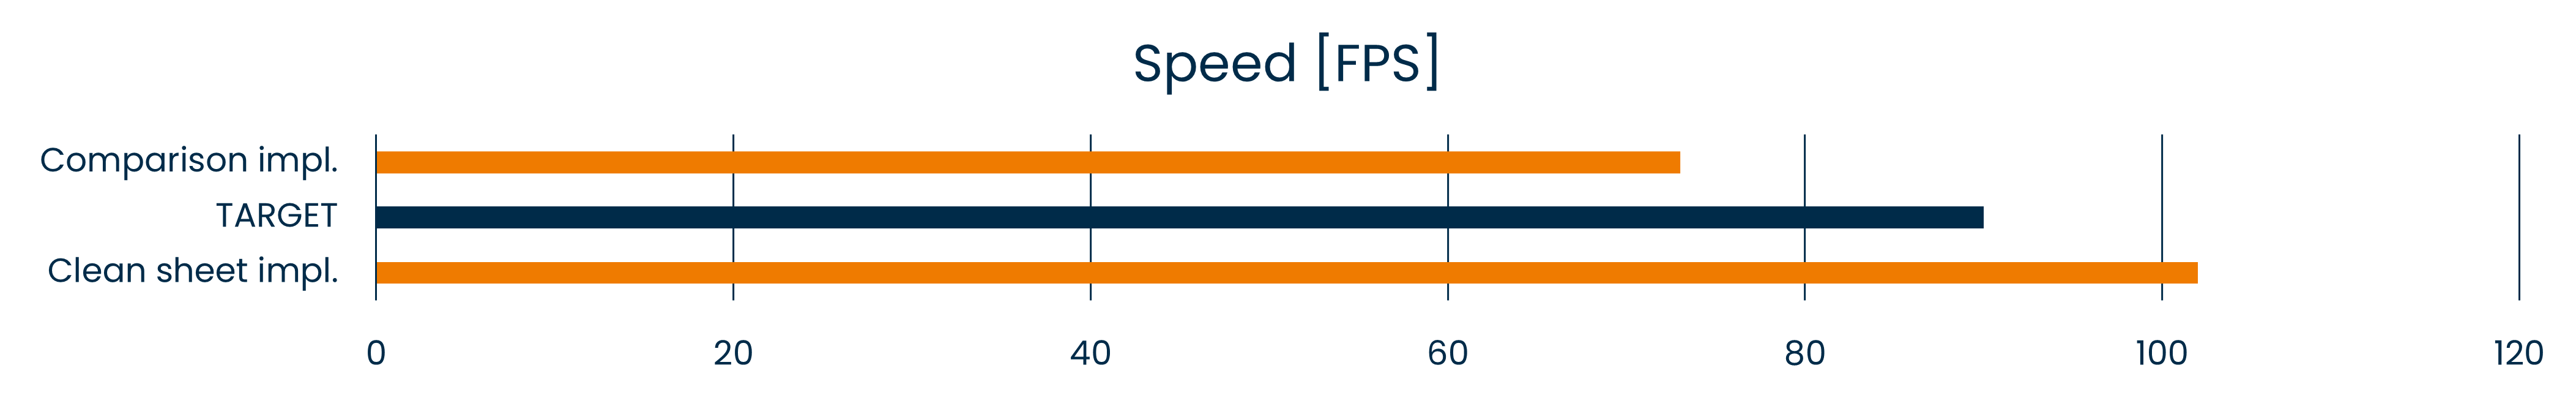
\includegraphics[width=\textwidth]{images/locate-cleansheet-speed.png}}
	\caption{\centering Computation speed of the chosen \textit{Locate} algorithm before and after the re-implementation, compared with the target speed.}
	\label{fig:locate:speed-cleansheet}
\end{figure}

\chapter{The \linkDD* step}
\label{chap:2dlink}

The \link* step aims to link together consecutive time instants, by joining the coordinates of each individual bubble across the various time instants it is seen.
The result is a series of trajectories, or \textbf{tracklets}.
Specifically, the 2D version of the \link* step operates on 2D coordinates, producing 2D tracklets.

\section{Requirements}

\subsection{Input}

The input to the \link* step coincides with the output of the previous step.
If the pipeline is using \linkDD*, the full pipeline under exam is \locate* - \link* - \match* - \visual*.
This means that the input to this step is the output of the \locate* step, as described in section~\ref{sec:locate:output}.

\subsection{Output}
\label{sec:linkDD:output}

The coordinates of the particles in the tracklets follow the same format as the \locate* output.
A four-dimensional \texttt{positions} array describes the \texttt{(x, y)} coordinates of the bubbles inside \texttt{positions[C][F][B]}, $C$, $F$ and $B$ being the camera, frame and bubble indices, respectively.
The difference with the \locate* format is that values of $B$ are scoped across the whole acquisition, not limited to the single frame.
This means that all values with the same $C$ and $B$ will represent the same real bubble across the different frames.

With this representation, valid bubbles are not clustered at the smallest values of $B$: for example, bubble $B{=}0$ may disappear after some frames, leaving the rest of its tracklet to contain invalid positions.
As such, the \texttt{numTracers} array is not anymore enough to describe the valid positions.
Instead, a different array is used: \texttt{validTracers} is a three-dimensional, boolean array.
\texttt{validTracers[C][F][B]} contains the information of whether the bubble $B$ of camera $C$ was detected at frame $F$.
False values indicate that, at a specific frame, the bubble was either not found yet, or already lost, or the overall number of bubbles traced by camera $C$ was lower than $B$.

\subsection{Speed}

As for the \locate* step, each second the \linkDD* has to process the bubbles from $N{\cdot}f$ frames, where $N$ is the number of cameras and $f$ is their frame rate.
As such, the required speed for this step is the same 90 FPS that is required by the \locate* step.

\subsection{Quality}

The overall quality of an algorithm can be estimated by combining manual observation with the number of resulting tracklets found.
For the manual observation, the input video was overlay-ed with a tail composed of points and segments, describing the last few frames of trajectory.
Figures~\ref{fig:linkDD:trackpy} and \ref{fig:linkDD:kalmangpu} are examples of frames used for manual observation: the single links are quite small, it is hard to see them individually, it's much easier to consider the general view.

Possible situations of reconstructed links are:
\begin{itemize}
	\itemsep 0em
	\item Link correctly detected: the number of total tracklets does not change from the previous frame, and the link is coherent with the rest of the trajectory;
	\item Link not detected: visually, it's hard to notice the missing link; however, this splits the tracklet into two pieces, increasing the number of tracklets by 1;
	\item Wrong link detected: the number of tracklets remains the same, while an inconsistent movement is visible by eye.
\end{itemize}
As such, a good reconstruction is one with few tracklets and a coherent visual representation.

\section{State of the art}

For the \link* step, online research was less successful: no new approach was found, and only some of the libraries found for the \locate* step were also performing the task:
\begin{itemize}
	\itemsep 0em
	\item Section~\ref{sec:link2d:trackpy} explores the Trackpy~\cite{trackpy} Python library;
	\item Section~\ref{sec:link2d:myptv} explores the MyPTV~\cite{myptv} Python library.
\end{itemize}
As for the \link* step, they are described and evaluated in the following chapters.

\section{Approaches}

The following sections describe the different approaches evaluated for the \linkDD* step.
They are evaluated on a 201-frames video~\cite{linkDD-original}, whose frames look like figure~\ref{fig:locate:original}.
For the different approaches, a crop of a sample frame is reported as per the \locate* approaches (section~\ref{sec:locate:approaches}), with the tail of the tracklet.
Full videos are available on YouTube, following the links in the corresponding citations.

\newpage
\subsection{Trackpy}
\label{sec:link2d:trackpy}

The \texttt{link} function from the Trackpy~\cite{trackpy} library is able to perform the \link* task both in 2D and in 3D.

Originally, it required the located positions to be inside a \texttt{Pandas Dataframe}, and it used to convert it into a \texttt{NumPy} array.
However, since our data was already inside a \texttt{NumPy} array with the same format, the library was altered to avoid this useless conversion, thus saving time.

\subsubsection{Algorithm}

The Trackpy library implements the Crocker-Grier linking algorithm~\cite{trackpy-link}.

\subsubsection{Evaluation}

For a single camera, the linking speed was 40 FPS.
If different cameras were analyzed in parallel processes, 3 cameras could be processed at an overall speed of 120 FPS.

The quality was good at a visual inspection (see figure~\ref{fig:linkDD:trackpy} or the full video~\cite{linkDD-trackpy}), and the total number of tracklets was around 6500.

\begin{figure}
	\centerline{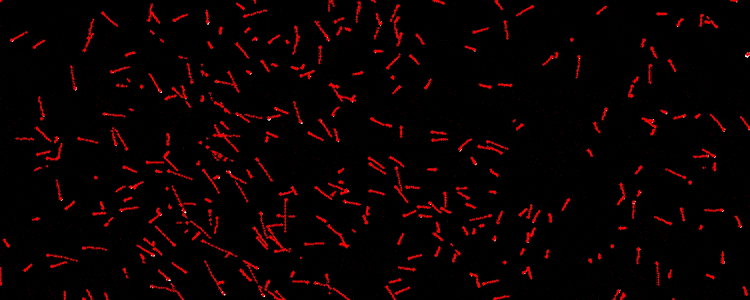
\includegraphics[width=\locateimgsize]{images/link2d/trackpy.png}}
	\caption{\centering A frame from the Trackpy \linkDD* result, full video available at~\cite{linkDD-trackpy}}
	\label{fig:linkDD:trackpy}
\end{figure}
 \newpage
\subsection{MyPTV}
\label{sec:link2d:myptv}

...

\subsubsection{Algorithm}

...

\subsubsection{Evaluation}

...

% \begin{figure}
% 	\centerline{\includegraphics[width=\locateimgsize]{images/link/...}}
% 	\caption{\centering ...'s result}
% 	\label{fig:locate:...}
% \end{figure}
 \newpage
\subsection{Kalman CPU}
\label{sec:link2d:kalman-cpu}

...

\subsubsection{Algorithm}

...

\subsubsection{Evaluation}

...

% \begin{figure}
% 	\centerline{\includegraphics[width=\locateimgsize]{images/link/...}}
% 	\caption{\centering ...'s result}
% 	\label{fig:locate:...}
% \end{figure}
 \newpage
\subsection{Kalman GPU}
\label{sec:link2d:kalman-gpu}

The Kalman CPU approach performs the same operation over all the bubbles of all the images.
A GPU implementation was therefore evaluated, to test its potential parallelization.

\subsubsection{Algorithm}

The algorithm is the same as the previous approach, with step 2 transformed into a GPU kernel.
This kernel processes all bubbles of all images captured at the same time instant.

\subsubsection{Evaluation}

The speed is quite faster than the Kalman CPU approach, but still considerably slower than Trackpy, standing at 68 FPS.
The quality was however worse: the number of tracklets increased to about 8900, and a visual inspection found some inconsistencies (in figure~\ref{fig:linkDD:kalmangpu}, two trackelts include an unreasonable jump).

\begin{figure}
	\centerline{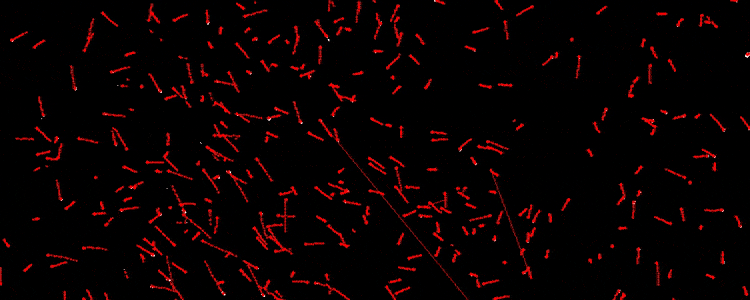
\includegraphics[width=\locateimgsize]{images/link2d/kalman_GPU.png}}
	\caption{\centering A frame from the Kalman GPU \linkDD* result, full video available at~\cite{linkDD-kalman-gpu}}
	\label{fig:linkDD:kalmangpu}
\end{figure}
 \newpage

\section{Final choice}

Figure~\ref{fig:linkDD:speed} compares the speeds of the various \linkDD* approaches: Trackpy is the only one with an adequate speed.
On top of that, it is also the approach with the best overall quality.
As such, if the pipeline is traversed in the \locate* - \link* - \match* - \visual* order, the \link* step will use the Trackpy implementation.

\begin{figure}
	\centerline{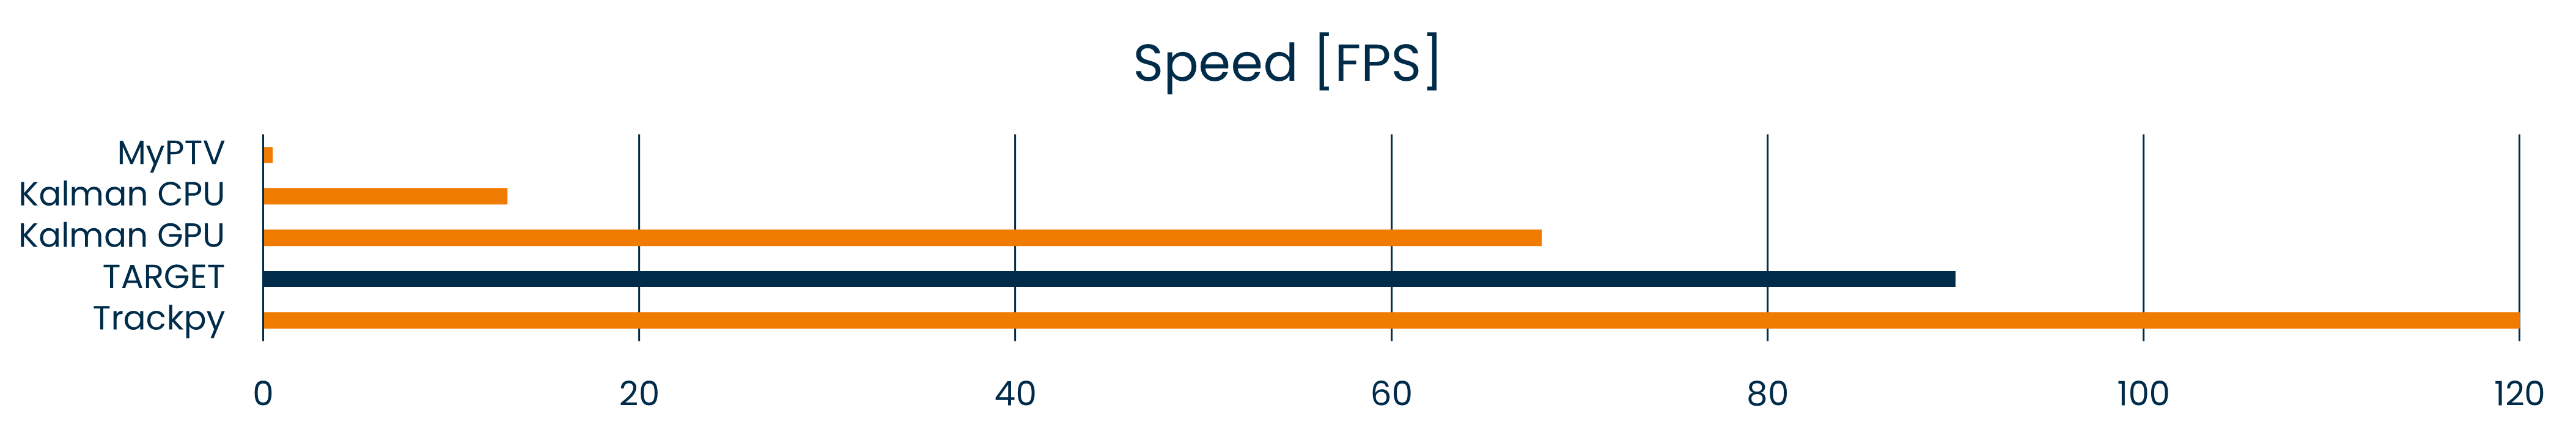
\includegraphics[width=\locateimgsize]{images/link2d-speed-comparison.png}}
	\caption{\centering Comparing the speeds of the different \linkDD* approaches}
	\label{fig:linkDD:speed}
\end{figure}

\chapter{The \match* step}
\label{chap:matching}

\section{Requirements}

\subsection{Input}

\subsection{Output}

\subsection{Speed}

\subsection{Quality}

\section{State of the art}

\section{Approaches}

\subsection{MyPTV}

\subsection{...}

\section{Final choice}

\chapter{The \textit{3D link} step}
\label{chap:3dlink}

\section{State of the art}
\section{Requirements}
\section{Approaches}
\subsection{MyPTV}
\subsection{...}
\section{Final choice}

\chapter{The Visualization step}
\label{chap:visual}

The goal of the \visual* step is to display the reconstructed 3D particles on a 2D screen, in the most understandable way.
Since no adequate tool was found on the Internet, the Unity renderer (explained in section~\ref{sec:visual:unity}) was initially developed as a versatile, offline tool.
After it was finished, an update to the requirements demanded for a renderer able to display the reconstruction as it was being done: the Open3D renderer (described in section~\ref{sec:visual:o3d}) was then added as an online alternative.

\section{Unity renderer}
\label{sec:visual:unity}

Displayed in figure~\ref{fig:visual:unity}, the Unity renderer is the first visualizer developed in the scope of this thesis.
It is an offline tool, meaning that it is able to show the data after the acquisition is fully processed.
The pipeline produces as output two \texttt{.npz} files, containing the arrays \texttt{positions} and \texttt{validTracers}.
These files can be directly loaded by the Unity scene setup to display their content.

A custom loader was necessary to transform the arrays from the \texttt{NumPy} format into C\# arrays.
Further modules are able to display such arrays in the 3d environment, using simple primitives as backbone.
In particular, the bubbles are represented by spheres in the 3D environment, connected by small rods to display the linked trajectories.

The time evolution of the bubbles is visible with real time: the user is able to ``play'' the scene for inspecting the general behavior.
The user also has control over the time speed, allowing to play back the experiment result in slow-motion, for better observing the fast-moving bubbles.
Alternatively, it is possible for the user to advance or go back by a single frame at a time, allowing to better inspect what happened at the smallest scale of time.

For better understanding the 3D position of the bubbles, the observer is able to move around the simulation.
% The user controls a camera that acts as a 
In particular, the user controls a ``floating camera'' that observes the scene from inside.
It is possible both to rotate the camera around its axes, and to move it.
The movement is possible in the direction where the camera is looking, and in the orthogonal, horizontal direction.
This movement ability allows the user to inspect the reconstruction from whichever angle they prefer.
Figure~\ref{fig:visual:cameradir} displays the way the user can move the visualization camera.

The simulation proposes some more controls to tailor the visualization to the needs of the user.
In particular, it is possible to customize at any time:
\begin{itemize}
	\itemsep 0em
	\item How many frames of trailing trajectory to display: 0, $N$ or all. This allows to concentrate on whatever is required at the moment: a specific time instant, a short-term evolution, or the full history.
	\item The size of the bubbles, that can be reduced up to make them disappear completely. This allows to either focus on the specific time instants where the frames were captured, or on the overall time evolution without focusing on the specific instants.
\end{itemize}

\begin{figure}[H]
	\centerline{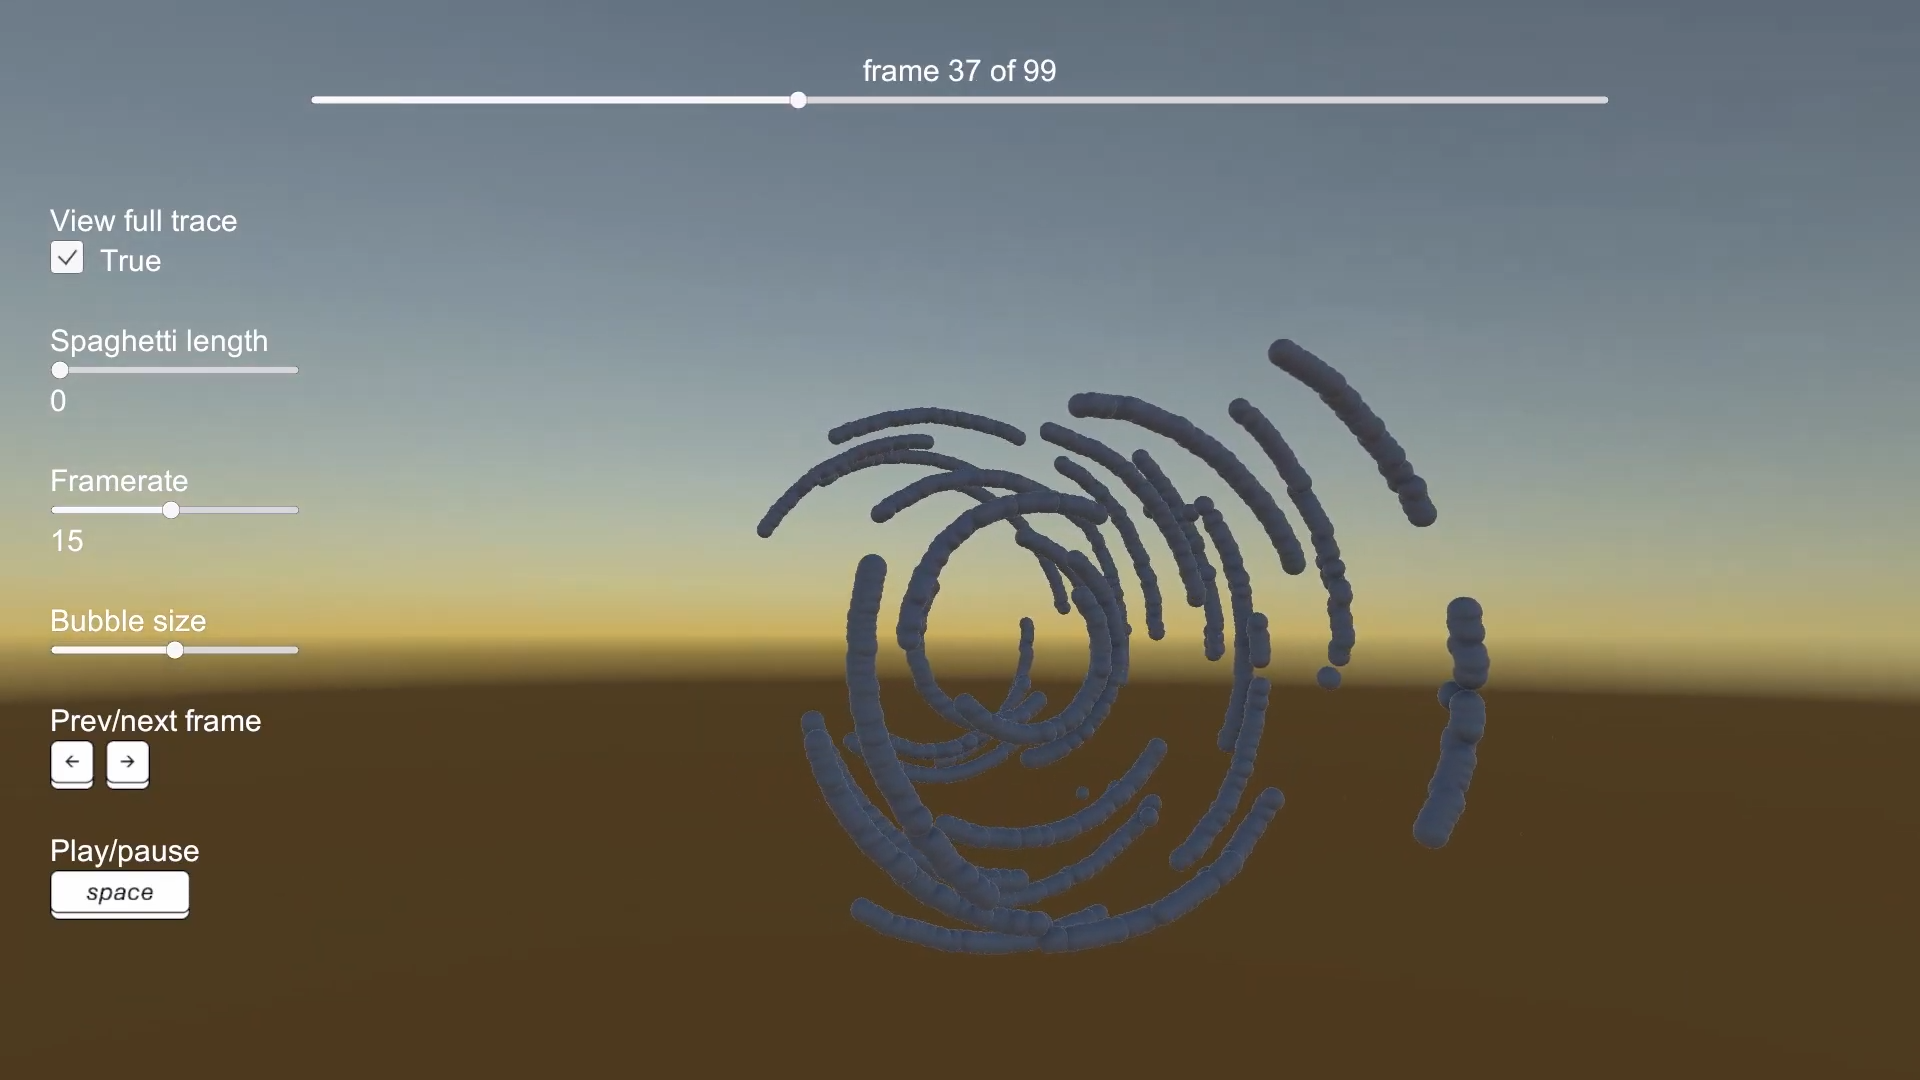
\includegraphics[width=\locateimgsize]{images/visual/unity.png}}
	\caption{\centering An example of bubble visualization using the Unity visualizer. Full video available at~\cite{visual-unity}}
	\label{fig:visual:unity}
\end{figure}

\begin{figure}[H]
	\centering
	\minipage{0.5\textwidth}
	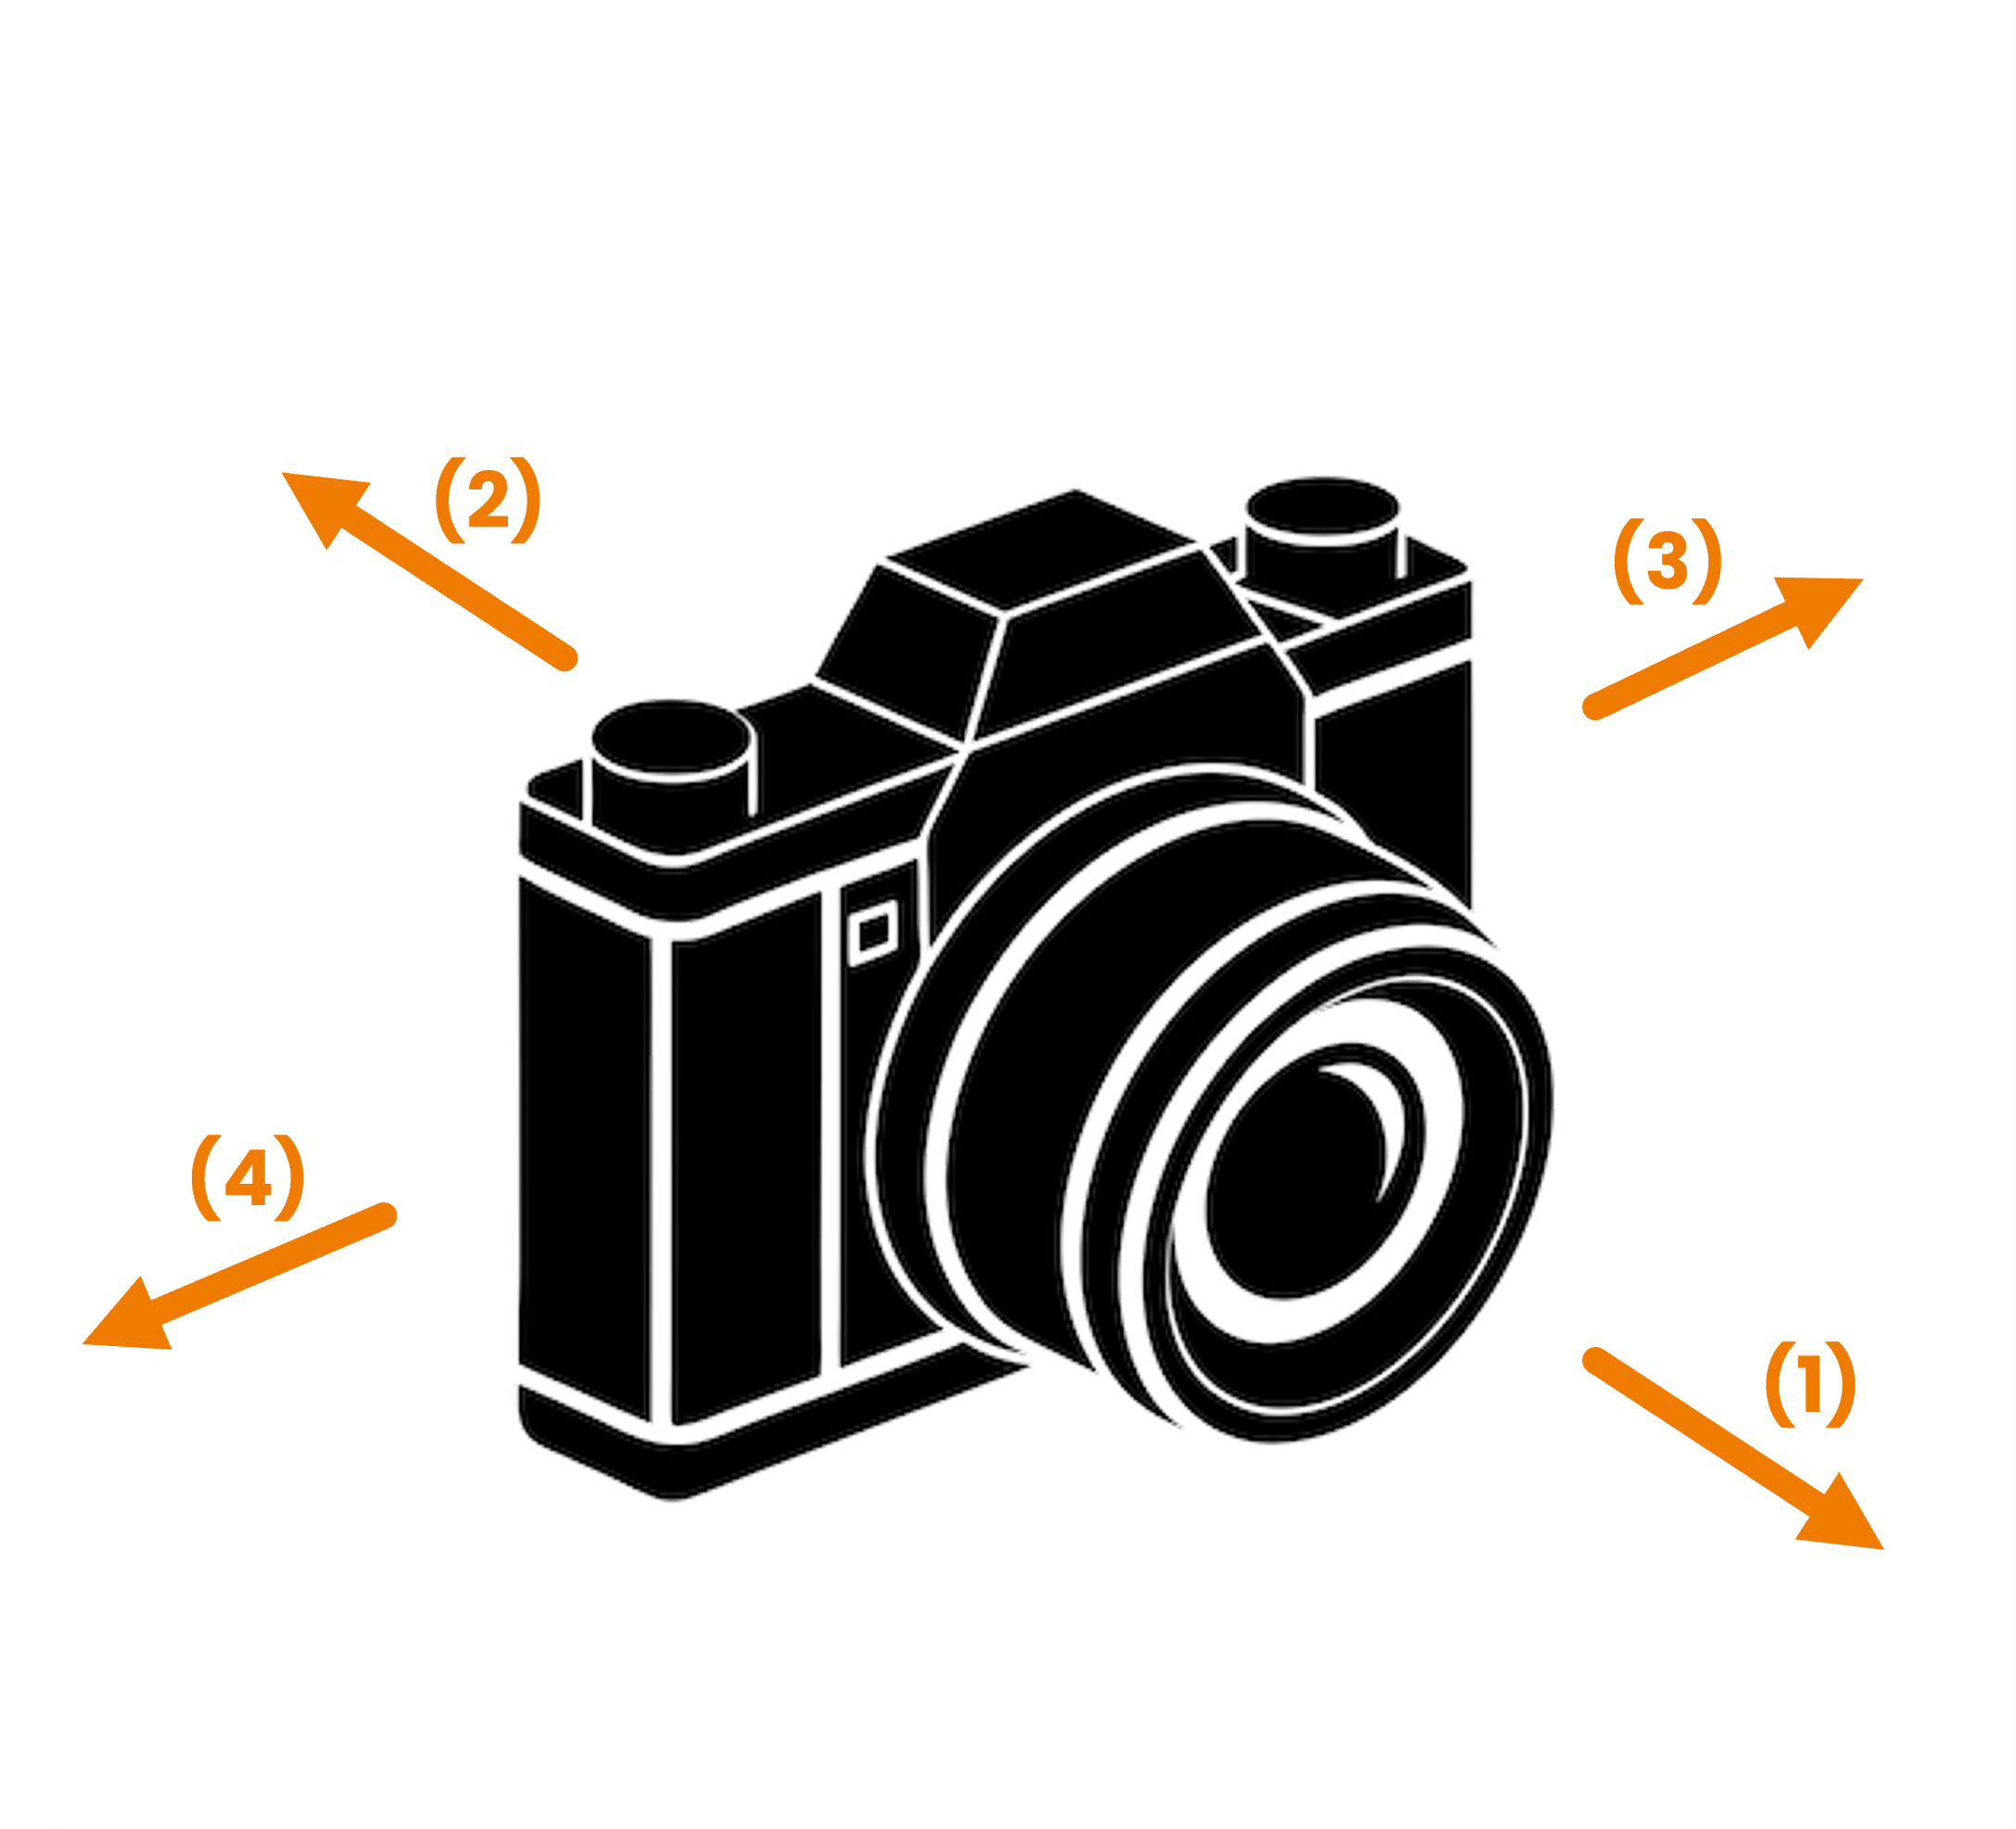
\includegraphics[width=\linewidth]{images/directions-of-moving.png}
	\endminipage\hfill
	\minipage{0.5\textwidth}
	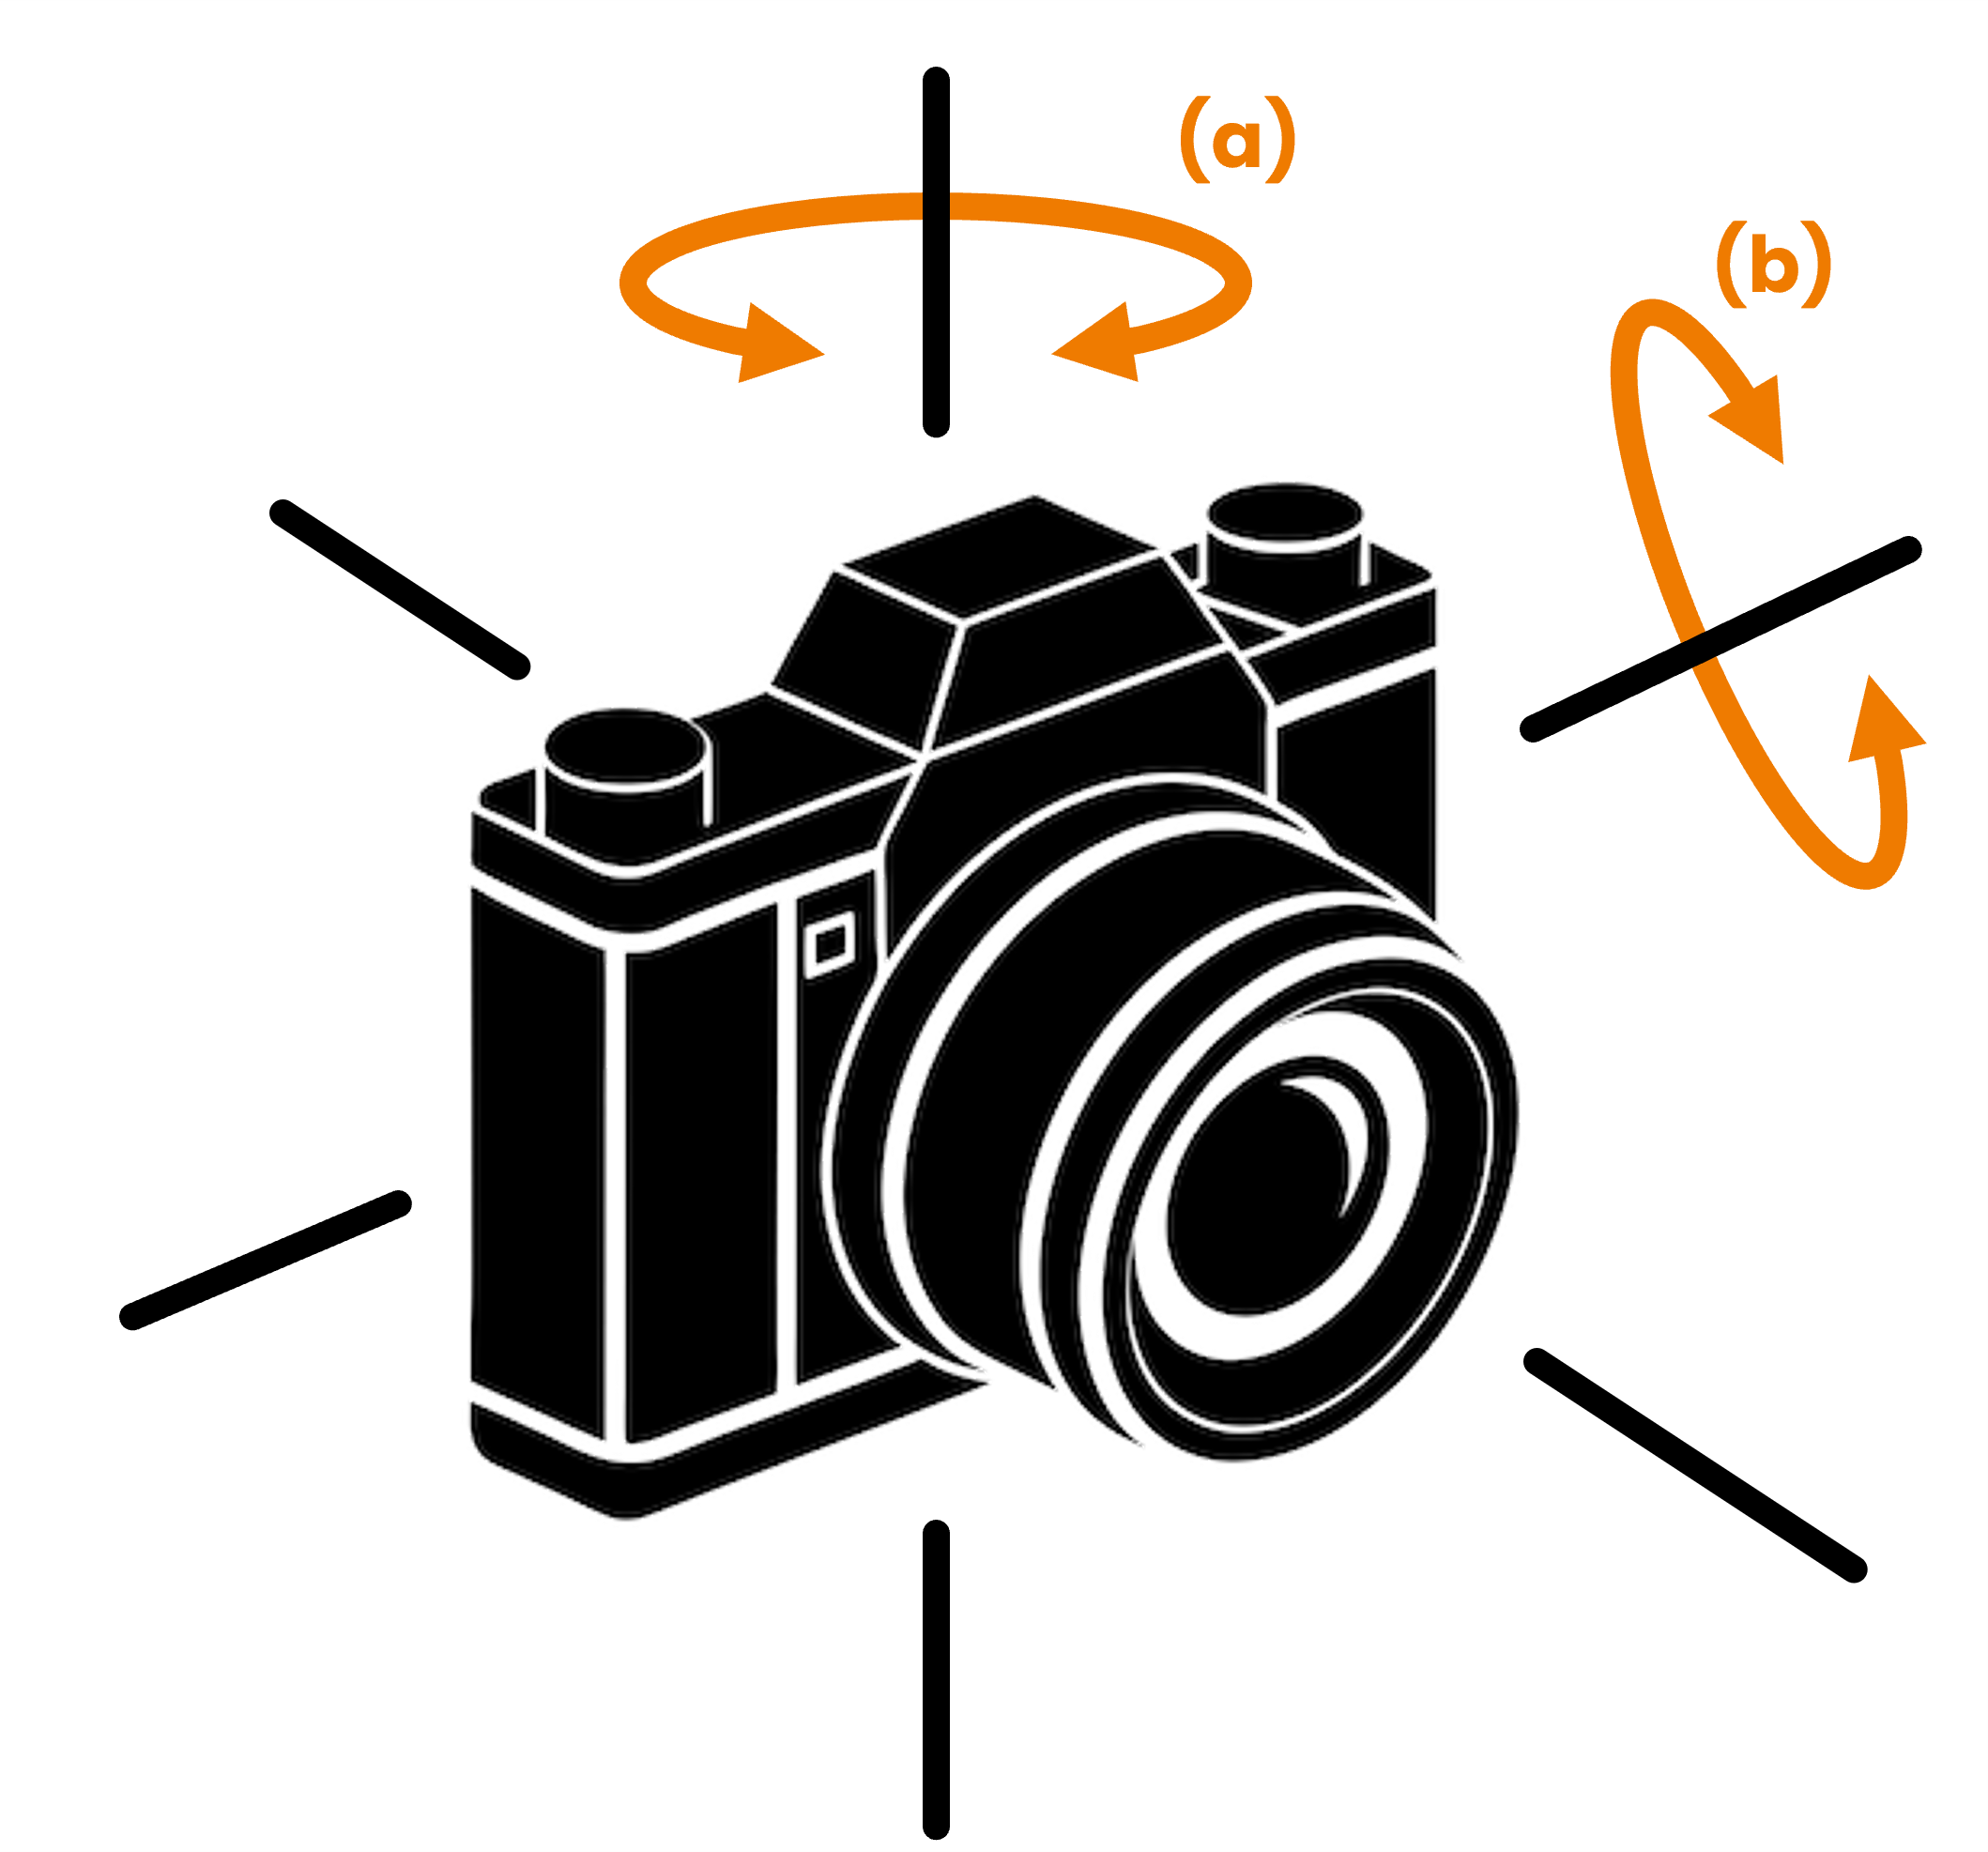
\includegraphics[width=\linewidth]{images/directions-of-rotating.png}
	\endminipage

	\caption{To the left, the four directions in which the user can move the visualization camera: (1) forward, (2) backwards, (3) left and (4) right, with respect of the current ``looking-at'' direction. To the right, the ways it can turn: (a) horizontally or (b) up and down}\label{fig:visual:cameradir}
\end{figure}

\section{Open3D renderer}
\label{sec:visual:o3d}

The Open3D renderer (a screenshot can be seen in figure~\ref{sec:visual:o3d}) was later added, to fulfill the requirements of an online renderer, meaning a renderer that would update in real-time, adding the new bubbles as soon as they are processed.

This was added as a separate step in the pipeline, taking the data directly from the last step.

The user movement is the same as in the Unity renderer (schema available in figure~\ref{fig:visual:cameradir}).
It may however be slightly laggy, since it's running on an embedded device, which at the same time is executing the rest of the pipeline.

Differently from the Unity renderer, this one cannot use real time as representation of reconstruction time: instead, a color gradient is used, with blue representing the first and red the last time instants.

Another drawback of this visualizer is its volatile nature: displaying the data as soon as it is computed, it is not possible to view back the result once the visualizer is closed.
In such cases, the Unity renderer can be used instead.

\begin{figure}
	\centerline{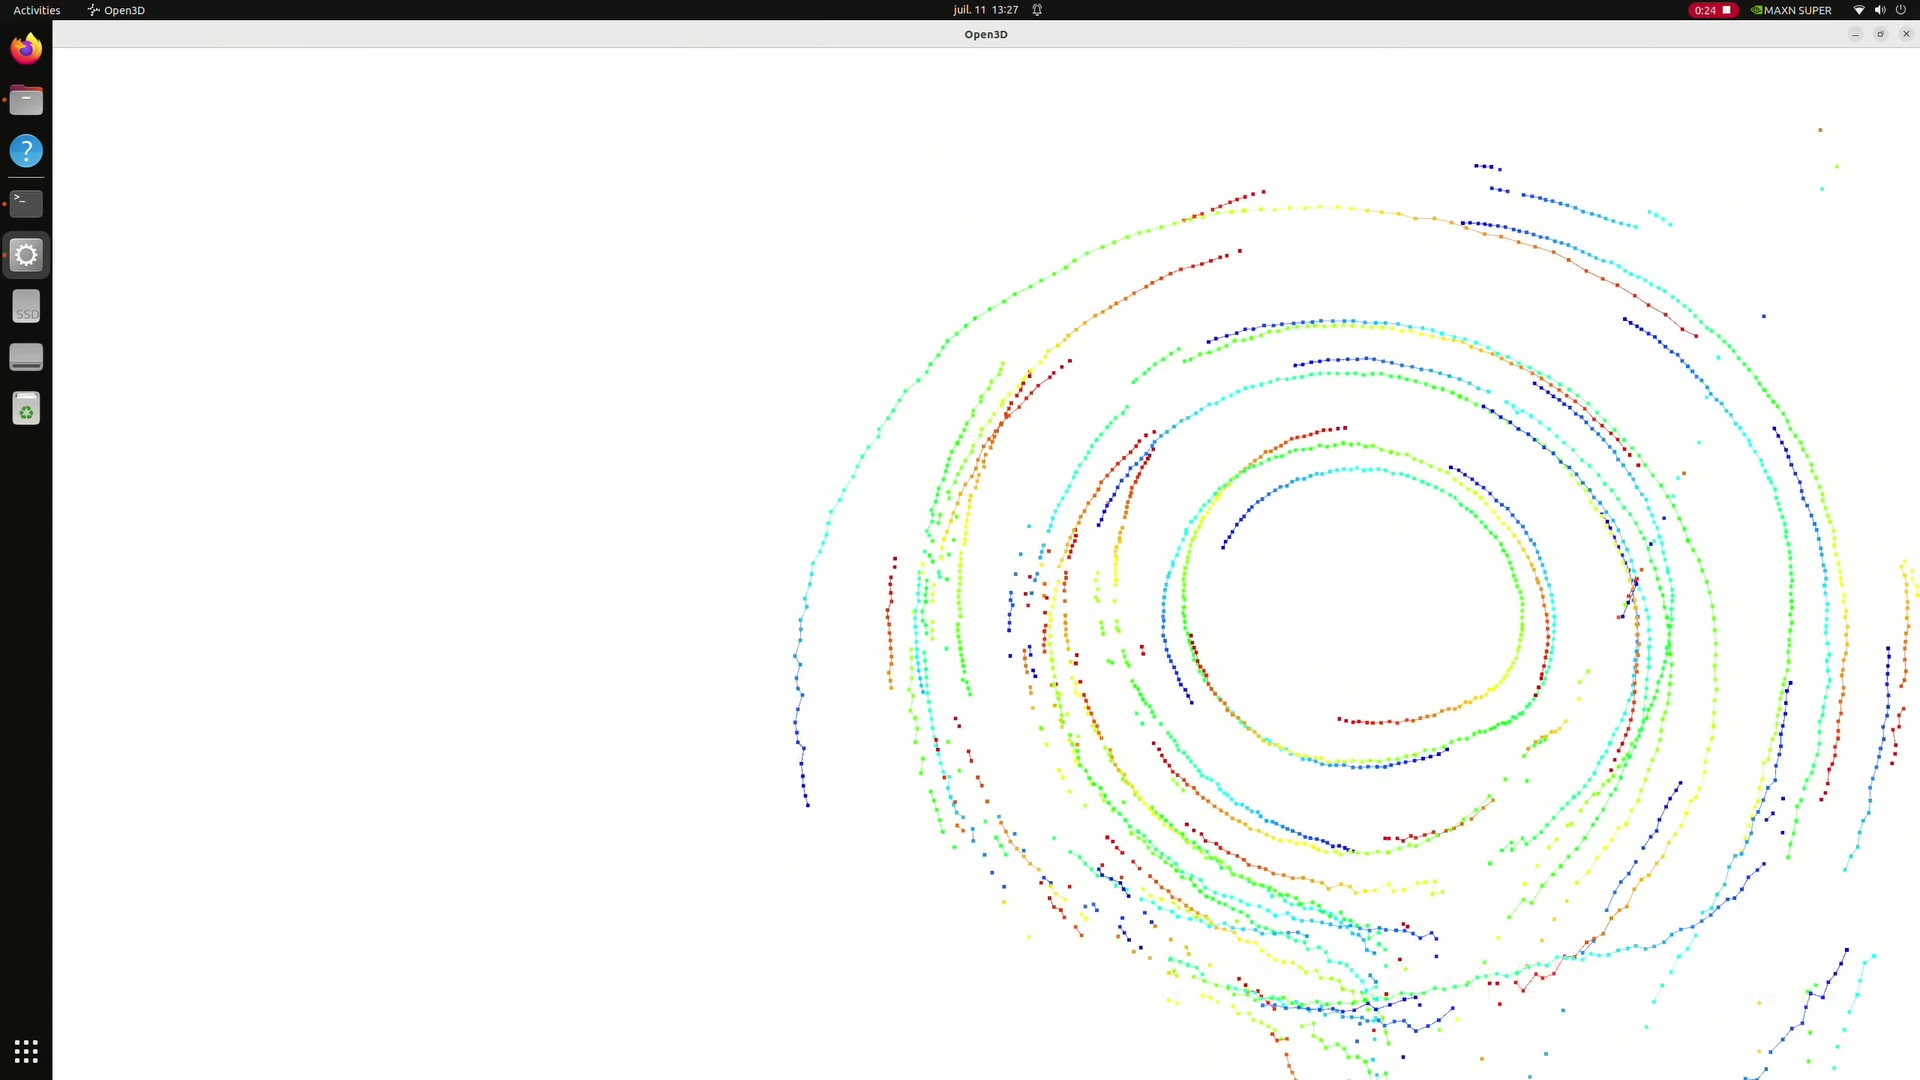
\includegraphics[width=\locateimgsize]{images/visual/o3d.png}}
	\caption{\centering An example of bubble visualization using the Open3D visualizer. Full video available at~\cite{visual-o3d}}
	\label{fig:visual:o3d}
\end{figure}

\chapter{The full pipeline}
\label{chap:pipeline}

\section{Pipeline order}

As described in chatper~\ref{chap:basicpipeline} and in figure~\ref{fig:pipeline:order} (reported here as figure~\ref{fig:pipeline:order-again} for convenience), the pipeline can be implemented either in the blue or in the orange order.

From the results of chatper~\ref{chap:3dlink}, the \linkDDD* (in the orange order) was quite faster than the \linkDD*: a faster step implies less computation resources used, which leaves more available for the most intensive tasks.
The other benefit of the orange pipeline is that the linking is performed in 3D, where more information are available.
In particular, it was noticed relatively often that the \match* step would reconstruct bubbles belonging to the same 2D tracklet at different depths, creating a sudden jump in the 3D trajectory, indicating an error.
Instead, when the \linkDDD* was used, the results were more coherent.
As such, the orange order was chosen for the pipeline.

\begin{figure}
	\centerline{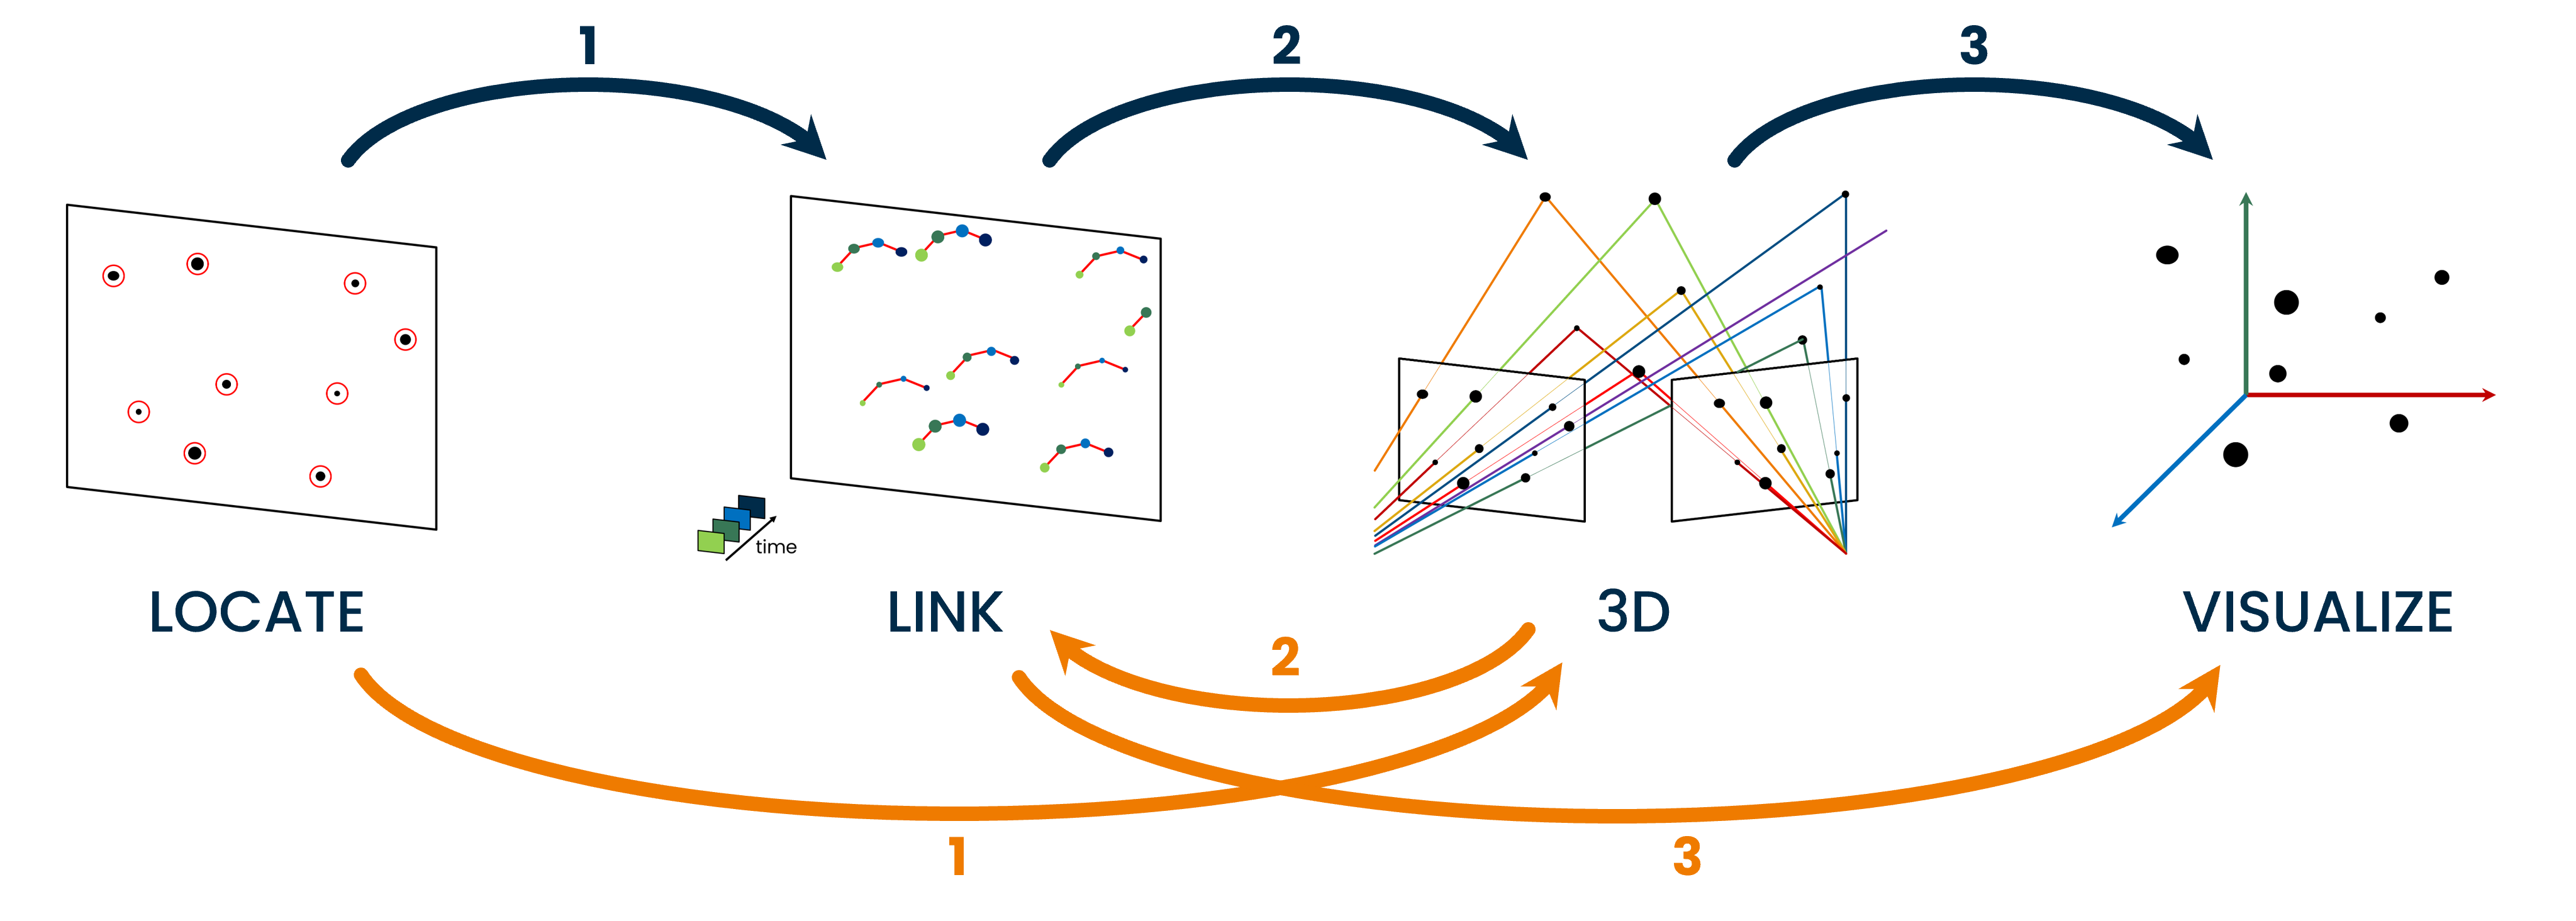
\includegraphics[width=\textwidth]{images/pipeline-orders.png}}
	\caption{\centering The two different orders in which the pipeline can be executed}
	\label{fig:pipeline:order-again}
\end{figure}

\section{Implementation}

The pipeline is implemented on the operating system as a set of processes, to fully use all the cores of the CPU.
Simpler threads would not be equivalent, since all Python threads are executed on the same CPU core.
The communication among the processes is realized by means of shared memory locations, where the input/output arrays are stored in a shared way.

The different processes are organized as follows:
\begin{itemize}
	\item the \locate* step is performed by its own process, that:
	      \begin{itemize}[topsep=0pt]
		      \itemsep 0em
		      \item loads the images either from the cameras or from file;
		      \item finds the bubbles using the \texttt{findContours} function;
		      \item launches and waits for the GPU computation of the moments.
	      \end{itemize}
	\item a process runs the \match* step, that:
	      \begin{itemize}[topsep=0pt]
		      \itemsep 0em
		      \item waits until new data is available from the \locate* step;
		      \item computes the first guess of matching;
		      \item computes the median displacement;
		      \item refines the first guess with the computed medians;
		      \item uses the matches to reconstruct 3D coordinates;
	      \end{itemize}
	\item the \link* (\linkDDD*) step is executed in another process, that:
	      \begin{itemize}[topsep=0pt]
		      \itemsep 0em
		      \item waits until new data is available from the \match* step;
		      \item performs the linking;
	      \end{itemize}
	\item if enabled, the \visual* step is run by a separate process, that:
	      \begin{itemize}[topsep=0pt]
		      \itemsep 0em
		      \item activates a new virtual environment, since \texttt{Open3D} requires a \texttt{NumPy} version not compatible with the rest;
		      \item runs the visualization script, that constantly checks for new values, displays them and responds to the user input.
	      \end{itemize}
	\item if enabled, a final debug process constantly updates the output in the terminal, writing the total number of frames processed by each step.
\end{itemize}
The different waits are realized as a loop that performs a 0.5s sleep until more data is available.

\chapter{Results}
\label{chap:results}

\section{Quality evaluation}

The main source of errors in the full pipeline is the \match* step, whose mistakes are then passed on to the \linkDDD* step.
The root cause to the \match* errors is the bubble density.
In fact, if few bubbles are present in the scene, there will be only a handful of candidates near the epiline.
This makes it trivial to choose the correct one, even with basic approaches.
As the bubble density increases, however, the number of candidates close to the epiline augments, too.
With that, the \match* task becomes harder and harder, reaching overwhelming levels also for a human at just 100 bubbles.
With every matching error, the algorithm reconstructs some ``random, isolated bubbles'' that not only are wrong by themselves, but also act as missing points in the trajectory chain, splitting the full trajectory into three separate parts.

% The main errors in the final pipeline are introduced in the \match* step, and then reflected onto the \linkDDD*.
% The main problem of the \match*  is the bubble density in the frames: with few bubbles, the epiline will not provide many candidates, thus making it easier to choose the correct match.
% As the density increases, the presence of more candidates implies more chance for mistakes, which would become ``random, isolated bubbles'' in the 3D view, which also break the trajectories reconstructed by the \link*.

For measuring how good the algorithm behaves with different bubble densities, some synthetic datasets were created in Blender, and used as input for the pipeline.
Such datasets were composed of 30 frames with the same format as the real ones: 960{$\times$}960 images, representing white bubbles over a black background.
The datasets were constructed to have a specific number of bubbles $N$, always visible by all the three cameras observing the scene.
All the bubbles rotate in a clockwise direction, with the same tangential speed: this enables to avoid bubbles shadowing each other, and creates a regular pattern that can be recognized by eye.
Given the specifications of the dataset, ideally the algorithm should be able to reconstruct exactly $N$ 30-frames-long trajectories: more trajectories are index of reconstruction errors.

% For measuring the quality as a function of the number of bubbles, different input datasets were developed in Blender, with the same format as the real data.
% In these datasets, a number $N$ of bubbles rotate in circles around the center of the image, never exiting the field of view of any camera for the full 30 frame duration.
% As such, the algorithm should be ideally able to reconstruct exactly $N$ tracklets with 30 frames of length.

As previously stated, the main source of errors is the \match*.
Errors at this stage position a bubble away from its correct location, splitting its trajectory in three parts.
In particular, for the 30-frames dataset, a single error at frame $f$ would split the full trajectory into two shorter segments, with lengths $f$ and $29-f$, plus a single-frame tracklet, with only the erroneous bubble.
As such, by analyzing the distribution of trajectory lengths, it is possible to evaluate the quality of the reconstruction.

% A single matching error at frame $f$ will move one bubble into the wrong position, splitting the 30-frame trajectory into three, with lenghts $f$, $1$ and $29-f$.
% As such, errors can be identified by examining the distribution of trajectory lenght.

Experiments were conducted with four different datasets, respectively with 50, 100, 250 and 1000 bubbles each.
% In particular, the x-axis contains the trajectory lenghts, and the corresponding y-value indicates the percentage of bubbles associated with a trajectory of such lenght.
% The x-value $x$ will be the percentage value of $N_x{\cdot}x:B$, where $B$ is the total number of bubbles of all frames, and $N_x$ is the number of trajectories with length $x$.
% The $x$ factor is crucial, since it makes the different lenghts comparable: without it, the graph would just be the percentage of tracklets with a specific lenght over the total number of tracklets.
% If that was the case, however, a full trajectory split into 3 pieces would be valued as three times a 
Initially, the graph in figure~\ref{fig:traj-len-distr} was created, with the most intuitive content: the percentage of trajectories with lenght $x$, for every possible length $x$.
This visualization was however misleading: for example, the 50-bubbles dataset had 29 full-lenght (30 frames) trajectories, which is more than half.
However, the corresponding point on the graph had a value of about 30\%.
The cause of this inconsistency in the graph is the fact that splitting a theoretical trajectory into smaller ones would increase the total number of trajectories, thus reducing all the percentages.
In other words, the correct reconstruction counts as 1, but a trajectory with an error in the middle counts as 3.
\begin{figure}
	\centerline{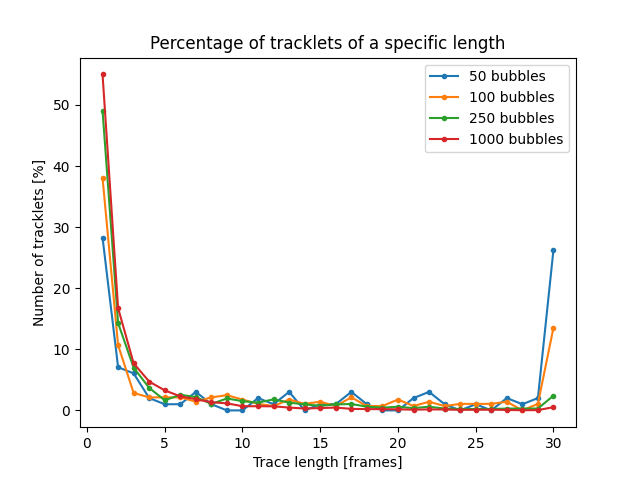
\includegraphics[width=0.7\textwidth]{images/traj-len-graph-first.png}}
	\caption{\centering The distribution of trajectory lengths for the different datasets with varying number of bubbles: considering each trajectory as ``one''}
	\label{fig:traj-len-distr}
\end{figure}

To make up for this error, a new graph was created, depicted in figure~\ref{fig:traj-len-distr-weighted}.
It does not compute the average over the number of trajectories, but over the number of bubbles, which is not affected by the reconstruction quality.
As such, the data points in this new graph are weighted over the trajectory lenght.
For example, a 1-long trajectory would count as a ``single unit'', while a 30-long trajectory has a value of ``30 units'' for this computation.
This enables to correctly showcase the overall quality of the reconstruction: in the 50-bubbles example considered before, now the value indicated by the graph for complete trajectories is about 60\%, coherent with the measure of 29 fully reconstructed tracklets over the total 50 bubbles.
\begin{figure}
	\centerline{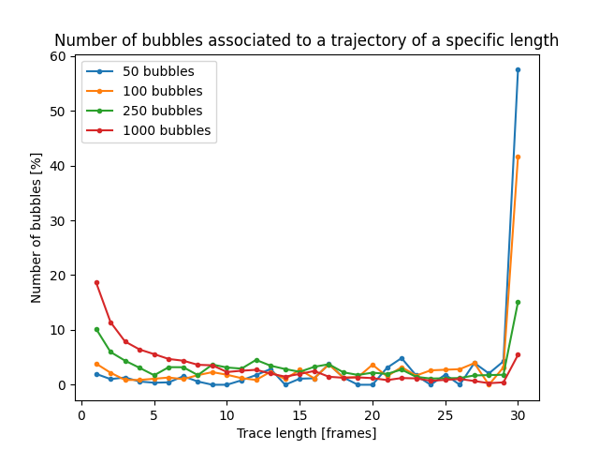
\includegraphics[width=0.7\textwidth]{images/traj-len-graph.png}}
	\caption{\centering The distribution of trajectory lengths for the different datasets with varying number of bubbles: considering trajectories weighted on their lenght}
	\label{fig:traj-len-distr-weighted}
\end{figure}

In the ideal scenario, both graphs should have a flat value of 0\% for all trajectory lengths, with a 100\% spike at the value 30: whatever departs from this is index of errors.
While it may seem counterintuitive, higher values (not 30) do not necessarily imply better results.
Assume there is a reconstruction error in a tracklet: instead of having a full, 30-frames trajectory, there will be 3, with lengths $f$, $1$ and $29-f$, with $f$ being the wrongly reconstructed frame.
By changing where the mistake was ($f$), the two peaks in the graph will move, spacing from 1 and 29 for $f{=}0$, to 14 and 15 for $f{=}14$.
There would however not be a real effect on the quality of the data: there will always be two coherent tracklets, separated by a missing point.
As such, values smaller than 30 indicate the presence of errors, without correlation between quality and individual lengths.

As visible in figure~\ref{fig:traj-len-distr-weighted}, in the first two datasets most of the tracklets cover the full length, while the quality diminishes visibly with the other datasets.
As such, the quality is considered good with observations of up to 100 bubbles.

% Figure~\ref{fig:traj-len-distr} compares such distribution of lengths for $N$ values of 50, 100, 250, 1000.
% The x axis represents the trajectory lenght, while the y axis is the percentage of bubbles associated with such lenght.
% For example, a 30-frames trajectory would count as ``30 units'' in the x=30 bin, while a trajectory split at frame 5 would count as 5 units at x=5, 1 unit at x=1 and 24 units at x=24.
% The percentage is obtained by dividing the value (in ``units'') of each bin by the total value of the graph, which is the total number of detected bubbles.
% Iteally, the graph should have value 0\% for all bins other than 30, which should have a value of 100\%.
% As visible in the graph, a good part of the trajectories is correct up to 100 bubbles, while adding more deteriorates the performance considerably.
% The quality is therefore considered good up to 100 bubbles.

\section{Speed evaluation}
\label{sec:results:speed}

\subsection{Overall speed}

The full pipeline took 42s to process a video composed of 1000 frames, thus resulting in a speed of 38 FPS, higher than what was required.
To avoid waiting times due to the camera frame rate, these measurements were computed by using a video previously captured and saved as set of frames on the disk.

\subsection{Speed of the pipeline steps}

As visible in figure~\ref{fig:speed:all-pipeline}, the process is 2.3x as fast as the initial SMA-RTY implementation, which was already faster than the provided Matlab script.
Naturally, the last step to complete is the last one of the pipeline, the \link*: however, as the next sections will show, the bottleneck is in the \locate* step.

\begin{figure}
	\centerline{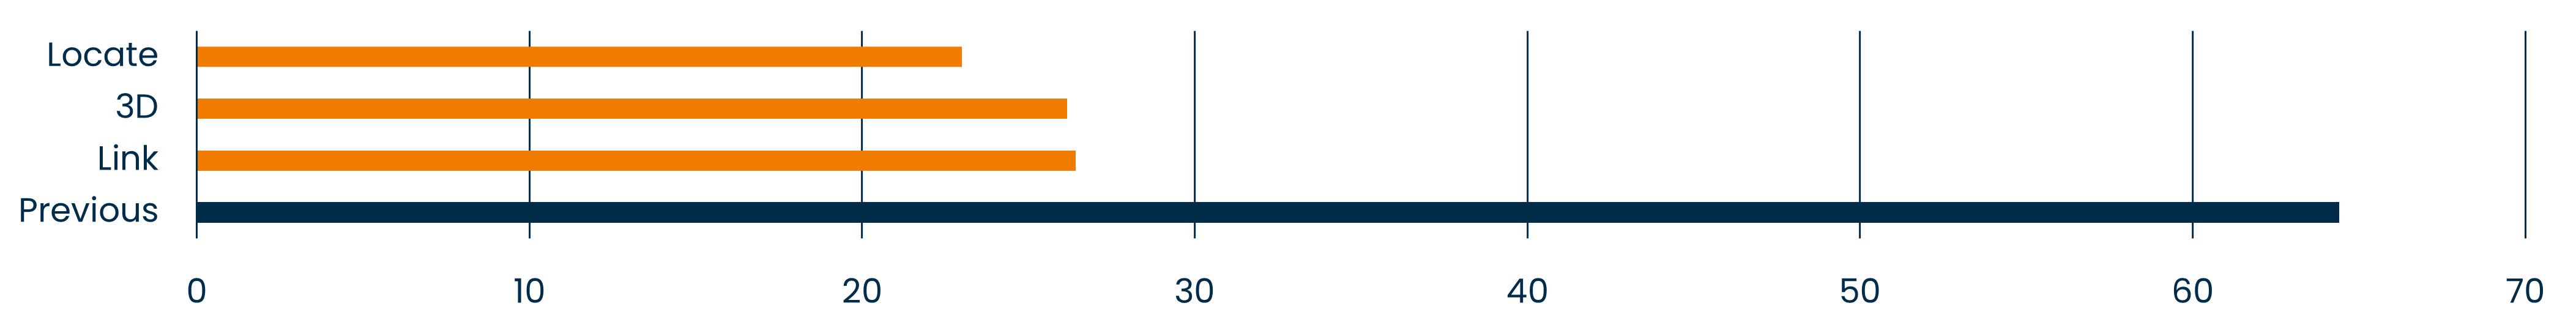
\includegraphics[width=\textwidth]{images/speed/overall-speed.png}}
	\caption{\centering The time required (in seconds) by the different pipeline steps to process a 1000-frames video}
	\label{fig:speed:all-pipeline}
\end{figure}

\subsubsection{\locate* step}

As shown in figure~\ref{fig:speed:locate}, the \locate* step was always fully operational, without ever having to wait for data.
This is obvious, since its input was already fully available at the start of the execution.
It must however be noted that, as visible in figure~\ref{fig:speed:all-pipeline}, the \locate* step did not finish much earlier than the others, indicating that it does not have a speed advantage over the other steps.

As visible in figure~\ref{fig:speed:locate}, the main bottleneck within this step is the time required for loading the images from the HDD to the RAM, to start processing them.

\begin{figure}
	\centerline{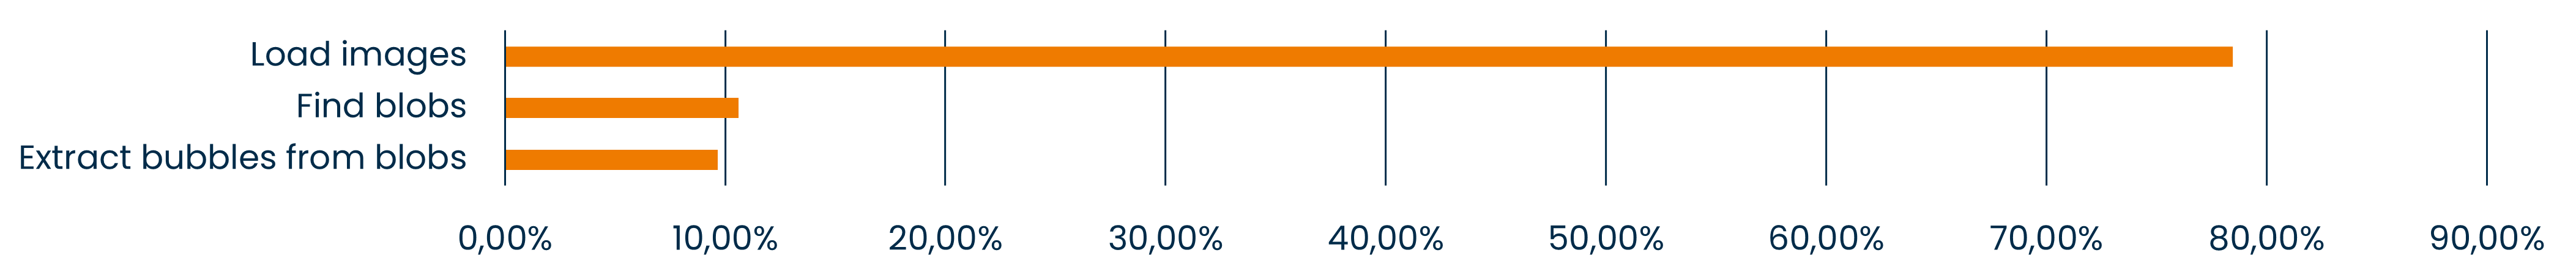
\includegraphics[width=\textwidth]{images/speed/locate.png}}
	\caption{\centering Distribution of how the \locate* step spent its execution time}
	\label{fig:speed:locate}
\end{figure}

\subsubsection{\match* step}

The \match* step, as visible in figure~\ref{fig:speed:match}, requires to spend a small amount of time waiting for the \locate* data.
This means that the \match* step is not the bottleneck.
The waiting time is however not extensive, indicating that even small slowdowns may make this step the bottleneck, affecting the whole pipeline performance.

\begin{figure}
	\centerline{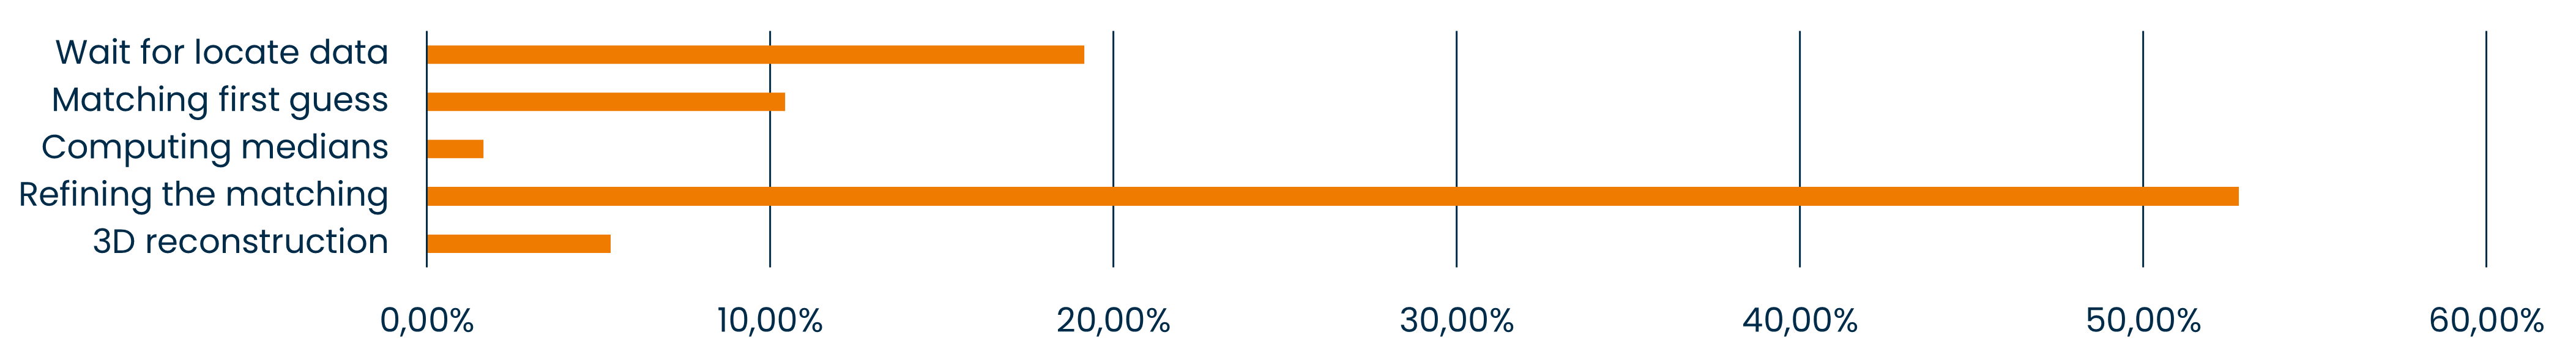
\includegraphics[width=\textwidth]{images/speed/matching.png}}
	\caption{\centering Distribution of how the \match* step spent its execution time}
	\label{fig:speed:match}
\end{figure}

\subsubsection{\link* step}

Figure~\ref{fig:speed:link} shows that most of the time the \link* step is idling, waiting for new inputs to be processed.
This indicates that it is far from being the bottleneck, and potentially more complex algorithm could be used instead, if they provided better results.

\begin{figure}[H]
	\centerline{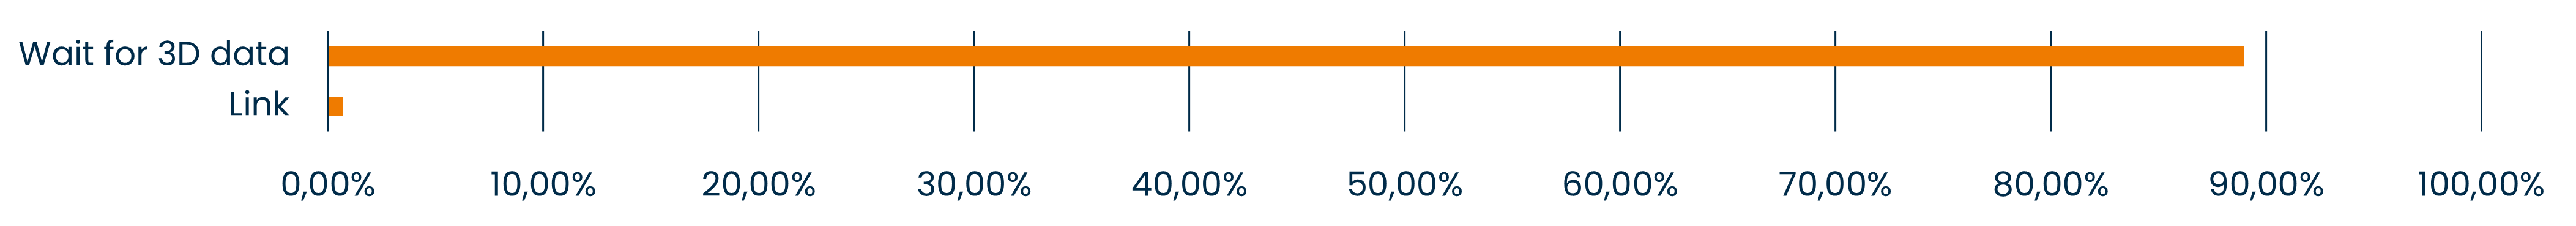
\includegraphics[width=\textwidth]{images/speed/link.png}}
	\caption{\centering Distribution of how the \link* step spent its execution time}
	\label{fig:speed:link}
\end{figure}

\subsection{Bottleneck evaluation}

As highlighted by the previous sections, the \locate* step is the current bottleneck of the system.
Figure~\ref{fig:pipeline-timing-schema} confirms this, by showing in a graphical way the timing of the different steps: the various \match* frames require to wait some time for the previous \locate* batches, and the \link* frames are constantly waiting for the \locate* output.

\begin{figure}[H]
	\centerline{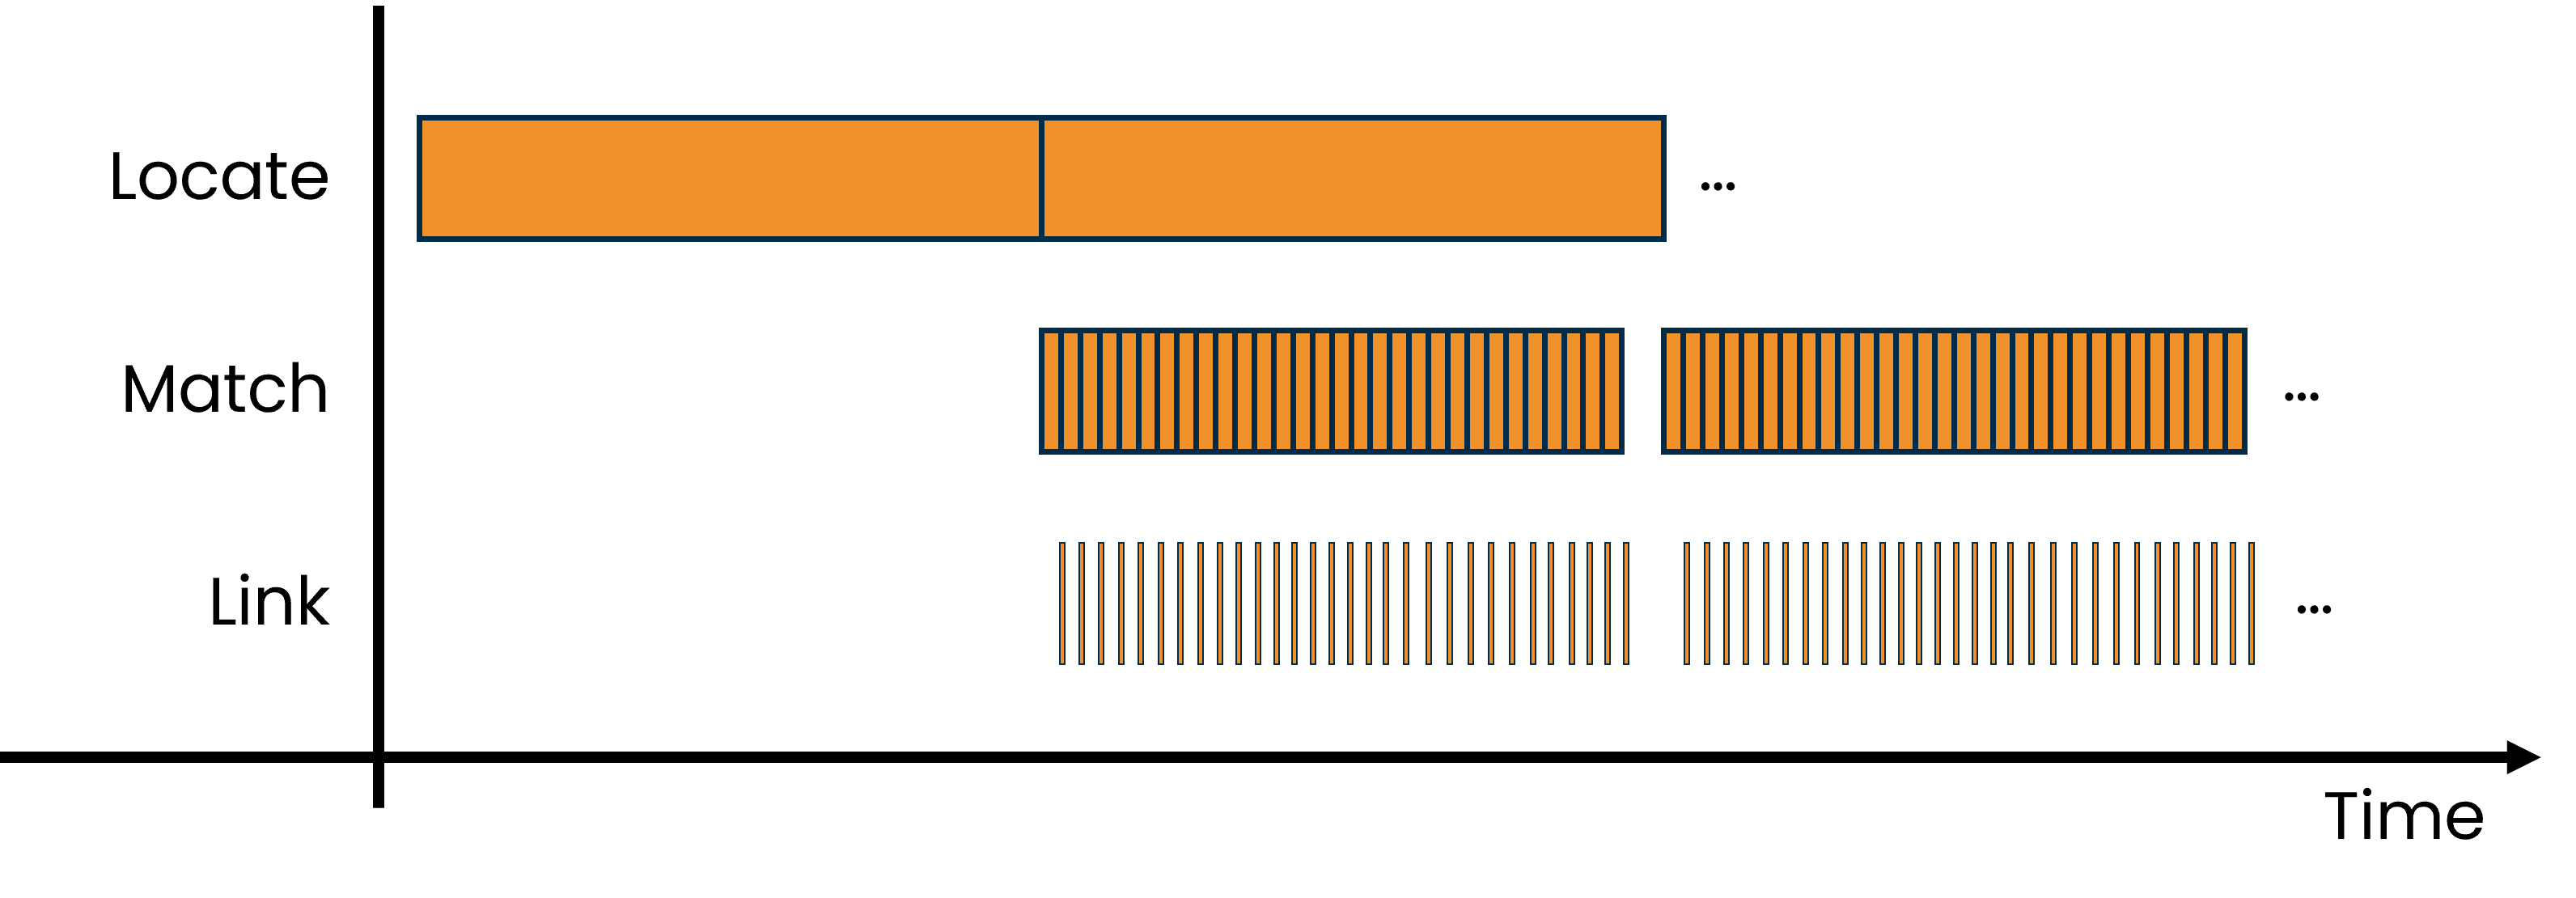
\includegraphics[width=.8\textwidth]{images/pipeline-timing.png}}
	\caption{\centering Schema (not to scale) of how the different pipeline stages are executed over time. The different rectangles indicate a batch of 20 frames per camera in the \locate*, and single frames in the other steps}
	\label{fig:pipeline-timing-schema}
\end{figure}
\newpage

\section{Resource usage}

A further test was conducted to measure the CPU usage of the device running the pipeline.
GPU usage was not measured, since the value would spike to 100\% as soon as there was any task running on it: the values would therefore not be indicative of whether other computations could be performed at the same time.
The CPU results are shown in figure~\ref{fig:usage}.

In the Jetson Orin Nano, all CPU cores are almost at 100\%, indicating that all resources are devolved to the task.
On the Jetson AGX Xavier, the situation is slightly different: the most notable fact is that the bottleneck shifts from the \locate* step to the \match*, and the overall processing speed is lower.
This is visible in the graph as a sudden de-loading of the device: when all steps are running, the full device is in use; after the \locate* finishes processing all the video, some cores reduce their usage.
This may be an indication that, being a more premium device, the Xavier is faster than the Orin at transferring data to the RAM; however the fact of being older penalyzes it on CPU computational speed.

\begin{figure}
	\captionsetup{list=false}

	\centering
	\minipage{0.5\textwidth}
	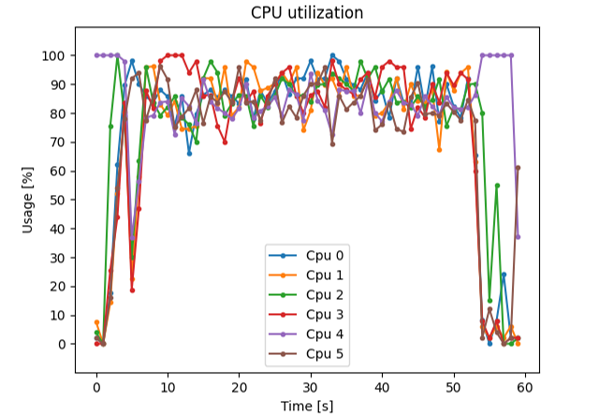
\includegraphics[width=\linewidth]{images/speed/usage-orin.png}
	\caption*{(a)}
	\endminipage\hfill
	\minipage{0.5\textwidth}
	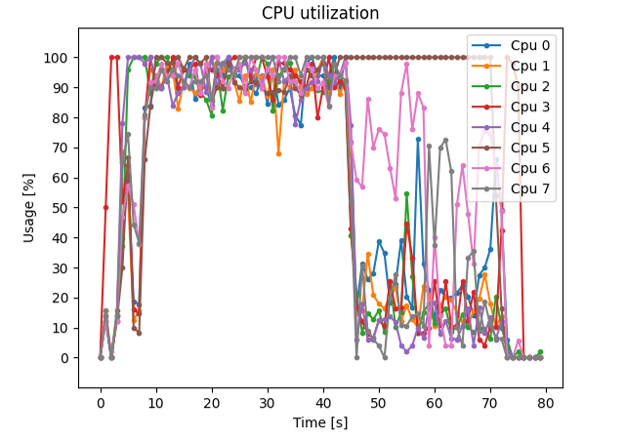
\includegraphics[width=\linewidth]{images/speed/usage-xavier.png}
	\caption*{(b)}
	\endminipage

	\captionsetup{list=true}

	\caption{\centering CPU usage per core, while running the pipeline on (a) the Jetson Orin Nano and (b) the Jetson AGX Xavier}\label{fig:usage}
\end{figure}


\chapter{Conclusions}
\label{chap:conclusions}

%\section{Result quality and speed}
Result quality and speed

\section{Future work}


% \paginavuota % it works even without stile=classica

%\appendix
%% appendix
\chapter{Galileo}
\label{sec:appendix_galileo}

\lstdefinelanguage{JavaScript}{
	keywords={break, case, catch, continue, debugger, default, delete, do, else, finally, for, function, if, in, const, instanceof, new, return, switch, this, throw, try, typeof, var, void, while, with},
	morecomment=[l]{//},
	morecomment=[s]{/*}{*/},
	morestring=[b]',
	morestring=[b]",
	sensitive=true
}

%\lstinputlisting[]{} % for source code files directly
% lstlisting environment for direct inclusion
\begin{lstlisting}[language=JavaScript]
    const test = test;
\end{lstlisting}

% for computational complexity
$\mathcal{O}\left(n\log{n}\right)$

% verbatim
\verb+numpy+



% endnotes here if needed

% \phantom{0}
\cleardoublepage
\printbibliography[heading=bibintoc] % heading required to show it in ToC

\end{document}
